\documentclass[12pt, openany, oneside]{book}

\usepackage{listings}
\usepackage[dvipsnames]{xcolor}
\usepackage{ctex}
\usepackage{fontspec}
\usepackage{setspace}
\usepackage{tikz}
\usepackage{anyfontsize}
\usepackage{sectsty}
\usepackage{titlesec}
\usepackage{float}
\usepackage[hidelinks]{hyperref}
\usepackage[a4paper]{geometry}
\usepackage{url}
\usepackage{amssymb}
\usepackage{fontawesome5}
\usepackage[most]{tcolorbox}
\usepackage{circuitikz}
\usepackage{stackengine}
\usepackage[edges]{forest}

\usetikzlibrary{calc,trees,positioning,arrows,fit,shapes}
\usetikzlibrary{shapes.multipart,chains}
\usetikzlibrary{arrows.meta}
\usetikzlibrary{decorations.pathmorphing}

\definecolor{land}{HTML}{95EA64}
\definecolor{water}{HTML}{BBE0E3}
\definecolor{bridge}{HTML}{FEFF9E}

\tikzset{
    contour/.style={
        very thick,
        decoration={
            random steps,
            segment length=4pt,
            amplitude=0.5pt
        },
        rounded corners=1pt,
        decorate
    }
}

\def\rlwd{.5pt} \def\rlht{2.2ex} \def\rldp{.5ex}
\def\mydiv#1{~
  \rule[-\rldp]{\rlwd}{\rlht}
  \setbox0=\hbox{~#1}
  \stackunder[\dimexpr\rldp-\rlwd]{~#1}{\rule{\wd0}{\rlwd}}%
}

\definecolor{mycolor}{RGB}{0,128,128}
\newtcbox{\mybox} {
    on line,
    colback=mycolor,
    fontupper=\bfseries\color{white},
    boxrule=0pt,
    arc=5pt, 
    boxsep=0pt, 
    left=2pt, 
    right=2pt, 
    top=5pt, 
    bottom=5pt
}

\setstretch{1.5}
\setlength{\parindent}{0cm}

\geometry{a4paper,top=2.5cm,bottom=2.5cm}

\titleformat{\chapter}{\Huge\Huge\bfseries}{\chaptertitlename\ \thechapter{\ }}{0pt}{\Huge}{}
\titlespacing{\chapter}{0pt}{0pt}{12pt}

\definecolor{dkgreen}{rgb}{0,0.4,0}
\definecolor{gray}{rgb}{0.5,0.5,0.5}
\definecolor{mauve}{rgb}{0.58,0,0.82}
\definecolor{LightGray}{gray}{0.9}

\tikzset{iv/.style={draw,fill=red!50,circle,minimum size=20pt,inner
sep=0pt,text=black},ev/.style={draw,fill=yellow,rectangle,minimum
size=20pt,inner sep=0pt,text=black}}

\lstset{
    basicstyle=\linespread{1.3} \fontspec{Consolas},    %  the size of the fonts that are used for the code
	basewidth=0.5em,
	numbers=left,            % where to put the line-numbers
    numberstyle=\color{black},  % the style that is used for the line-numbers
    numbersep=10pt,                  % how far the line-numbers are from the code
    backgroundcolor=\color{white},
    showspaces=false,
    showstringspaces=false,
    showtabs=false,
    frame=single,                   % adds a frame around the code
    rulecolor=\color{black},        % if not set, the frame-color may be changed on line-breaks within not-black text (e.g. commens (green here))
    tabsize=4,                      % sets default tabsize to 2 spaces
    captionpos=t,                   % sets the caption-position to bottom
    breaklines=false,                % sets automatic line breaking
    breakatwhitespace=true,        % sets if automatic breaks should only happen at whitespace
    title=\lstname,                   % show the filename of files included with \lstinputlisting;
    % also try caption instead of title
    numberstyle=\color{black},		% line number color
    keywordstyle=\color{blue},          % keyword style
    commentstyle=\color{dkgreen},       % comment style
    stringstyle=\color{mauve},         % string literal style
    escapeinside={\%*}{*)},            % if you want to add LaTeX within your code
    morekeywords={*,...}               % if you want to add more keywords to the set
}

\begin{document}

\thispagestyle{empty}

\begin{tikzpicture}[overlay,remember picture]
	\fill[
		black!2]
	(current page.south west) rectangle (current page.north east);

	\shade[
		left color=Dandelion,
		right color=Dandelion!40,
		transform canvas ={rotate around ={45:($(current page.north west)+(0,-6)$)}}]
	($(current page.north west)+(0,-6)$) rectangle ++(9,1.5);

	\shade[
		left color=lightgray,
		right color=lightgray!50,
		rounded corners=0.75cm,
		transform canvas ={rotate around ={45:($(current page.north west)+(.5,-10)$)}}]
	($(current page.north west)+(0.5,-10)$) rectangle ++(15,1.5);

	\shade[
		left color=lightgray,
		rounded corners=0.3cm,
		transform canvas ={rotate around ={45:($(current page.north west)+(.5,-10)$)}}] ($(current page.north west)+(1.5,-9.55)$) rectangle ++(7,.6);

	\shade[
		left color=orange!80,
		right color=orange!60,
		rounded corners=0.4cm,
		transform canvas ={rotate around ={45:($(current page.north)+(-1.5,-3)$)}}]
	($(current page.north)+(-1.5,-3)$) rectangle ++(9,0.8);

	\shade[
		left color=red!80,
		right color=red!80,
		rounded corners=0.9cm,
		transform canvas ={rotate around ={45:($(current page.north)+(-3,-8)$)}}] ($(current page.north)+(-3,-8)$) rectangle ++(15,1.8);

	\shade[
		left color=orange,
		right color=Dandelion,
		rounded corners=0.9cm,
		transform canvas ={rotate around ={45:($(current page.north west)+(4,-15.5)$)}}]
	($(current page.north west)+(4,-15.5)$) rectangle ++(30,1.8);

	\shade[
		left color=RoyalBlue,
		right color=Emerald,
		rounded corners=0.75cm,
		transform canvas ={rotate around ={45:($(current page.north west)+(13,-10)$)}}]
	($(current page.north west)+(13,-10)$) rectangle ++(15,1.5);

	\shade[
		left color=lightgray,
		rounded corners=0.3cm,
		transform canvas ={rotate around ={45:($(current page.north west)+(18,-8)$)}}]
	($(current page.north west)+(18,-8)$) rectangle ++(15,0.6);

	\shade[
		left color=lightgray,
		rounded corners=0.4cm,
		transform canvas ={rotate around ={45:($(current page.north west)+(19,-5.65)$)}}]
	($(current page.north west)+(19,-5.65)$) rectangle ++(15,0.8);

	\shade[
		left color=OrangeRed,
		right color=red!80,
		rounded corners=0.6cm,
		transform canvas ={rotate around ={45:($(current page.north west)+(20,-9)$)}}]
	($(current page.north west)+(20,-9)$) rectangle ++(14,1.2);

	% Title
	\node[align=center] at ($(current page.center)+(0,-7)$)
	{
	{\fontsize{72}{72} \selectfont {{离散数学}}}\\[1cm]
	{\fontsize{42}{42} \selectfont {{Discrete Mathematics}}}\\[2cm]
	{\fontsize{20}{19.2} \selectfont \textcolor{orange}{ \bf 极夜酱}}\\[4pt]
	};
\end{tikzpicture}

\newpage

\pagestyle{plain}
\setcounter{page}{1}
\setcounter{tocdepth}{1}
\tableofcontents

\newpage

\setcounter{page}{1}

\chapter{逻辑}

\section{命题}

\subsection{命题(Proposition)}

逻辑(logic)规则给出数学语句的准确含义,这些规则用来区分有效和无效的数学论证。逻辑不仅对理解数学推理十分重要,而且在计算机科学中有许多应用,逻辑可用于电路设计、程序构造、程序正确性证明等方面。\\

命题是逻辑的基本成分,一个命题是一个具有真值(truth value)的语句,命题可以为真也可以为假,但不能既为真又为假。

\begin{table}[H]
	\centering
	\setlength{\tabcolsep}{5mm}{
		\begin{tabular}{|c|c|}
			\hline
			\textbf{命题}        & \textbf{非命题}    \\
			\hline
			I have a dog.        & What day is today? \\
			\hline
			1 + 2 = 3            & Shut the door!     \\
			\hline
			Today is Wednesday.  & 1 + 2              \\
			\hline
			It is snowing today. & x + 1 = 2          \\
			\hline
		\end{tabular}
	}
	\caption{命题与非命题}
\end{table}

命题习惯上用字母$ p $, $ q $, $ r $, $ s $等来表示,如果一个命题是真命题,它的真值为真,用T表示;如果一个命题是假命题,它的真值为假,用F表示。\\

\subsection{非运算符(NOT, Negation Operator)}

非运算符$ \neg $只作用于一个命题,其作用是反转命题的真值。\\

真值表(truth table)可以给出命题真值之间的关系,在确定由简单命题组成的命题的真值时,真值表特别有用。

\begin{table}[H]
	\centering
	\setlength{\tabcolsep}{5mm}{
		\begin{tabular}{|c|c|}
			\hline
			\textbf{$ p $} & \textbf{$ \neg p $} \\
			\hline
			T              & F                   \\
			\hline
			F              & T                   \\
			\hline
		\end{tabular}
	}
	\caption{NOT真值表}
\end{table}

\begin{tcolorbox}
	\mybox{Exercise}
	$ \neg p $\\
	$ p $: It snowed last night.\\
	$ \neg p $: It didn;t snow last night.\\
	$ q $: $ 2 + 3 = 6 $\\
	$ \neg q $: $ 2 + 3 \ne 6 $
\end{tcolorbox}

\vspace{0.5cm}

\subsection{合取运算符(AND, Conjunction Operator)}

命题$ p \wedge q $表示$ p $并且$ q $,当$ p $和$ q $都为真时命题为真,否则为假。

\begin{table}[H]
	\centering
	\setlength{\tabcolsep}{5mm}{
		\begin{tabular}{|c|c|c|}
			\hline
			\textbf{$ p $} & \textbf{$ q $} & \textbf{$ p \wedge q $} \\
			\hline
			T              & T              & T                       \\
			\hline
			T              & F              & F                       \\
			\hline
			F              & T              & F                       \\
			\hline
			F              & F              & F                       \\
			\hline
		\end{tabular}
	}
	\caption{AND真值表}
\end{table}

\begin{tcolorbox}
	\mybox{Exercise}
	$ p \wedge q $\\
	$ p $: 今天是星期五。\\
	$ q $: 今天会下雨。\\
	$ p \wedge q $: 今天是星期五并且会下雨。
\end{tcolorbox}

\vspace{0.5cm}

\subsection{析取运算符(OR, Disjunction Operator)}

命题$ p \vee q $表示$ p $或$ q $,当$ p $和$ q $都为假时命题为假,否则为真。

\begin{table}[H]
	\centering
	\setlength{\tabcolsep}{5mm}{
		\begin{tabular}{|c|c|c|}
			\hline
			\textbf{$ p $} & \textbf{$ q $} & \textbf{$ p \vee q $} \\
			\hline
			T              & T              & T                     \\
			\hline
			T              & F              & T                     \\
			\hline
			F              & T              & T                     \\
			\hline
			F              & F              & F                     \\
			\hline
		\end{tabular}
	}
	\caption{OR真值表}
\end{table}

\begin{tcolorbox}
	\mybox{Exercise}
	$ p \vee q $\\
	$ p $: 开关坏了。\\
	$ q $: 灯泡坏了。\\
	$ p \vee q $: 开关坏了或者灯泡坏了。
\end{tcolorbox}

\vspace{0.5cm}

\subsection{异或运算符(XOR, Exclusive Or)}

命题$ p \oplus q $表示$ p $和$ q $的异或,当$ p $和$ q $中恰有一个为真时命题为真,否则为假。

\begin{table}[H]
	\centering
	\setlength{\tabcolsep}{5mm}{
		\begin{tabular}{|c|c|c|}
			\hline
			\textbf{$ p $} & \textbf{$ q $} & \textbf{$ p \oplus q $} \\
			\hline
			T              & T              & F                       \\
			\hline
			T              & F              & T                       \\
			\hline
			F              & T              & T                       \\
			\hline
			F              & F              & F                       \\
			\hline
		\end{tabular}
	}
	\caption{XOR真值表}
\end{table}

\begin{tcolorbox}
	\mybox{Exercise}
	$ p \oplus q $\\
	$ p $: 他现在在上海。\\
	$ q $: 他现在在北京。\\
	$ p \vee q $: 他现在在上海或北京。
\end{tcolorbox}

\begin{tcolorbox}
	\mybox{Exercise}
	某地发生了一件谋杀案,警察通过排查确定杀人凶手必为4个嫌疑犯的一个,根据以下信息确定凶手。\\
	A说:不是我。\\
	B说:是C。\\
	C说:是D。\\
	D说:C在胡说。\\
	已知3个人说了真话,1个人说的是假话。
\end{tcolorbox}

\begin{lstlisting}[language=Python]
def main():
    for killer in ['A', 'B', 'C', 'D']:
        if (killer != 'A') + (killer == 'C') \
            + (killer == 'D') + (killer != 'D') == 3:
            print(killer)

if __name__ == "__main__":
    main()
\end{lstlisting}

\begin{tcolorbox}
	\mybox{运行结果}
	C
\end{tcolorbox}

\newpage

\section{复合命题}

\subsection{复合命题(Compound Proposition)}

使用非运算符和已定义的各联结词可以构造复合命题。小括号用于规定复合命题中多个逻辑运算符的操作顺序,为了减少所需的小括号数量,规定了各联结词的优先级。

\begin{table}[H]
	\centering
	\setlength{\tabcolsep}{5mm}{
		\begin{tabular}{|c|c|}
			\hline
			\textbf{优先级} & \textbf{运算符}                   \\
			\hline
			1               & $ \neg $                          \\
			\hline
			2               & $ \wedge $ / $ \vee $             \\
			\hline
			3               & $ \rightarrow / \leftrightarrow $ \\
			\hline
		\end{tabular}
	}
	\caption{运算符优先级}
\end{table}

\vspace{0.5cm}

\subsection{蕴含运算符(Implication Operator)}

命题$ p \rightarrow q $表示$ p $蕴含$ q $,在$ p $为真而$ q $为假时命题为假,否则为真。其中$ p $称为前提,$ q $称为结论。

\begin{table}[H]
	\centering
	\setlength{\tabcolsep}{5mm}{
		\begin{tabular}{|c|c|c|}
			\hline
			\textbf{$ p $} & \textbf{$ q $} & \textbf{$ p \rightarrow q $} \\
			\hline
			T              & T              & T                            \\
			\hline
			T              & F              & F                            \\
			\hline
			F              & T              & T                            \\
			\hline
			F              & F              & T                            \\
			\hline
		\end{tabular}
	}
	\caption{蕴含真值表}
\end{table}

表示$ p \rightarrow q $的术语有很多种,常见的有:

\begin{itemize}
	\item If $ p $, then $ q $.
	\item $ p $ only if $ q $.
	\item $ q $ is necessary for $ p $.
\end{itemize}

\begin{tcolorbox}
	\mybox{Exercise}
	$ p \rightarrow q $\\
	$ p $:我去看电影。\\
	$ q $:我买奶茶。\\
	$ p \rightarrow q $:如果我去看电影,那么我会买奶茶。
\end{tcolorbox}

\begin{figure}[H]
	\centering
	
\includegraphics[scale=0.7]{img/C1/1-2/1.png}
\end{figure}

由$ p \rightarrow q $可以构造出几个相关的蕴含:

\begin{enumerate}
	\item $ q \rightarrow p $称为$ p \rightarrow q $的逆命题(converse)。
	\item $ \neg q \rightarrow \neg p $称为$ p \rightarrow q $的逆否命题(contrapositive)。
\end{enumerate}

\begin{tcolorbox}
	\mybox{Exercise}
	逆命题与逆否命题\\
	$ p $:今天是星期四。\\
	$ q $:我今天有考试。\\
	$ p \rightarrow q $:如果今天是星期四,那么我今天有考试。\\
	$ q \rightarrow p $:如果我今天有考试,那么果今天是星期四。\\
	$ \neg q \rightarrow \neg p $:如果我今天没有考试,那么今天不是星期四。
\end{tcolorbox}

\vspace{0.5cm}

\subsection{双向蕴含(Biconditional Operation)}

命题$ p \leftrightarrow q $表示$ p $双向蕴含$ q $,在$ p $和$ q $有相同的真值时命题为真,否则为假。

\begin{table}[H]
	\centering
	\setlength{\tabcolsep}{5mm}{
		\begin{tabular}{|c|c|c|}
			\hline
			\textbf{$ p $} & \textbf{$ q $} & \textbf{$ p \leftrightarrow q $} \\
			\hline
			T              & T              & T                                \\
			\hline
			T              & F              & F                                \\
			\hline
			F              & T              & F                                \\
			\hline
			F              & F              & T                                \\
			\hline
		\end{tabular}
	}
	\caption{双向蕴含真值表}
\end{table}

双蕴含的真值表与异或的真值表正好相反,因此$ p \leftrightarrow q $与$ \neg (p \oplus q) $等价。

\newpage

\section{逻辑等价}

\subsection{逻辑等价(Logical Equivalence)}

两个不同的复合命题可能拥有完全相同的真值,则称这两个命题在逻辑上是等价的。如果无论复合命题中各个命题的真值是什么,复合命题的真值总是为真,这样的复合命题称为永真式(tautology)。如果真值永远为假的复合命题称为矛盾(contradiction)。

\begin{table}[H]
	\centering
	\setlength{\tabcolsep}{5mm}{
		\begin{tabular}{|c|c|c|c|}
			\hline
			\textbf{$ p $} & \textbf{$ \neg p $} & \textbf{$ p \vee \neg p $} & \textbf{$ p \wedge \neg p $} \\
			\hline
			T              & F                   & T                          & F                            \\
			\hline
			F              & T                   & T                          & F                            \\
			\hline
		\end{tabular}
	}
	\caption{逻辑等价}
\end{table}

如果复合命题$ s $和是$ r $逻辑等价的,可表示为$ s \equiv r $。只有当$ s \leftrightarrow r $是永真式时,$ s $和$ r $才是逻辑等价的。

\begin{tcolorbox}
	\mybox{Exercise}
	使用真值表证明$ p \vee q \equiv \neg (\neg p \wedge \neg q) $
	\begin{table}[H]
		\centering
		\setlength{\tabcolsep}{5mm}{
			\begin{tabular}{|c|c|c|c|c|c|c|}
				\hline
				\textbf{$ p $} & \textbf{$ q $} & \textbf{$ p \vee q $} & \textbf{$ \neg p $} & \textbf{$ \neg q $} & \textbf{$ \neg p \wedge \neg q $} & \textbf{$ \neg (\neg p \wedge \neg q) $} \\
				\hline
				T              & T              & T                     & F                   & F                   & F                                 & T                                        \\
				\hline
				T              & F              & T                     & F                   & T                   & F                                 & T                                        \\
				\hline
				F              & T              & T                     & T                   & F                   & F                                 & T                                        \\
				\hline
				F              & F              & F                     & T                   & T                   & T                                 & F                                        \\
				\hline
			\end{tabular}
		}
	\end{table}
\end{tcolorbox}

\vspace{0.5cm}

\subsection{逻辑等价定理}

\begin{tcolorbox}
	\mybox{幂等律 Idempotent Laws}
	\begin{align}
		p \wedge p & \equiv p \\
		p \vee p   & \equiv p
	\end{align}
\end{tcolorbox}

\begin{tcolorbox}
	\mybox{恒等律 Identity Laws}
	\begin{align}
		p \wedge T & \equiv p \\
		p \vee F   & \equiv p
	\end{align}
\end{tcolorbox}

\begin{tcolorbox}
	\mybox{支配律 Domination Laws}
	\begin{align}
		p \vee T   & \equiv T \\
		p \wedge F & \equiv F
	\end{align}
\end{tcolorbox}

\begin{tcolorbox}
	\mybox{双非律 Double Negation Law}
	\begin{align}
		\neg (\neg p) & \equiv p
	\end{align}
\end{tcolorbox}

\begin{tcolorbox}
	\mybox{交换律 Commutative Laws}
	\begin{align}
		p \wedge q & \equiv q \wedge p \\
		p \vee q   & \equiv q \vee p
	\end{align}
\end{tcolorbox}

\begin{tcolorbox}
	\mybox{结合律 Associative Laws}
	\begin{align}
		(p \wedge q) \wedge r & \equiv p \wedge (q \wedge r) \\
		(p \vee q) \vee r     & \equiv p \vee (q \vee r)
	\end{align}
\end{tcolorbox}

\begin{tcolorbox}
	\mybox{分配律 Distributive Laws}
	\begin{align}
		(p \wedge q) \wedge r & \equiv p \wedge (q \wedge r) \\
		(p \vee q) \vee r     & \equiv p \vee (q \vee r)
	\end{align}
\end{tcolorbox}

\begin{tcolorbox}
	\mybox{德摩根律 De Morgan's Laws}
	\begin{align}
		\neg (p \wedge q) & \equiv \neg p \vee \neg q   \\
		\neg (p \vee q)   & \equiv \neg p \wedge \neg q
	\end{align}
\end{tcolorbox}

\begin{tcolorbox}
	\mybox{吸收律 Absorption Laws}
	\begin{align}
		p \wedge (p \vee q) & \equiv p \\
		p \vee (p \wedge q) & \equiv p
	\end{align}
\end{tcolorbox}

\begin{tcolorbox}
	\mybox{条件恒等}
	\begin{align}
		p \rightarrow q     & \equiv \neg p \vee q                              \\
		p \leftrightarrow q & \equiv (p \rightarrow q) \wedge (q \rightarrow p)
	\end{align}
\end{tcolorbox}

\begin{tcolorbox}
	\mybox{Exercise}
	证明$ (p \vee q) \rightarrow p $永真
	\begin{align*}
		 & (p \vee q) \rightarrow p           \\
		 & \equiv \neg (p \wedge q) \vee p    \\
		 & \equiv (\neg p \vee \neg q) \vee p \\
		 & \equiv (\neg q \vee \neg p) \vee p \\
		 & \equiv \neg q \vee (\neg p \vee p) \\
		 & \equiv \neg q \vee T               \\
		 & \equiv T
	\end{align*}
\end{tcolorbox}

\newpage

\section{谓词与量词}

\subsection{谓词(Predicate)}

命题逻辑并不能表达数学语言和自然语言中所有语句的确切含义。在数学表达式和计算机程序中经常可以看到含有变量的语句,例如$ x > 3 $、$ x = y + 3 $、程序$ x $正在运行等。当变量值未指定时,这些语句既不为真也不为假。\\

利用$ P(x) $可以表示语句,其中$ x $是变量,语句$ P(x) $可以说是命题函数$ P $在$ x $的值。一旦给变量$ x $赋一个值,语句$ P(x) $就称为命题并具有真值。\\

通常使用大写字母$ P $, $ Q $, $ R $等表示谓词,小写字母$ x $, $ y $, $ z $等表示变量。

\begin{tcolorbox}
	\mybox{Exercise}
	谓词
	\begin{table}[H]
		\centering
		\setlength{\tabcolsep}{5mm}{
			\begin{tabular}{|l|l|}
				\hline
				\textbf{谓词}          & \textbf{真值}      \\
				\hline
				$ P(x): x + 3 = 6 $    & $ P(3) $为True     \\
				\hline
				$ Q(x, y): x = y + 2 $ & $ Q(4, 1) $为False \\
				\hline
			\end{tabular}
		}
	\end{table}
\end{tcolorbox}

\vspace{0.5cm}

\subsection{量词(Quantifier)}

量词用量化表示在何种程度上谓词对于一定范围的个体成立。量词有全称量词(universal quantifier)和存在量词(existential quantifer)。\\

全称量词$ \forall $表示all。$ \forall_x P(x) $是一个命题,当范围内所有的$ x $都能使语句$ P(x) $为真时,命题为真。

\vspace{-0.5cm}

$$
	\forall_x P(x) = P(a_1) \wedge P(a_2) \wedge \dots \wedge P(a_k)
$$

\begin{tcolorbox}
	\mybox{Exercise}
	全称量词\\
	假设$ x $表示全班所有学生,$ P(x) $表示$ x $完成了作业。\\
	$ \forall_x P(x) $:全班所有学生都完成了作业。
\end{tcolorbox}

存在量词$ \exists $表示exists。$ \exists_x P(x) $是一个命题,当范围内存在至少一个$ x $能够语句$ P(x) $为真时,命题为真。

\vspace{-0.5cm}

$$
	\exists_x P(x) = P(a_1) \vee P(a_2) \vee \dots \vee P(a_k)
$$

\begin{tcolorbox}
	\mybox{Exercise}
	存在量词\\
	假设$ x $表示全班所有学生,$ P(x) $表示$ x $完成了作业。\\
	$ \exists_x P(x) $:班里存在有一个学生完成了作业。
\end{tcolorbox}

\begin{tcolorbox}
	\mybox{Exercise}
	嵌套量词\\
	假设$ x $表示某个人,$ P(x) $表示有父母。\\
	$ \forall_x P(x) $:所有人都有父母。\\
	$ \exists_x \neg P(x) $:存在至少有一个人没有父母。\\
	$ \exists_x \exists_y (P(x) \wedge P(y)) $:至少存在一个人$ x $和一个人$ y $有父母。
\end{tcolorbox}

\begin{tcolorbox}
	\mybox{Exercise}
	$ P(x) $:$ x $是偶数,$ Q(x) $:$ x $能被3整除,$ x \in \mathbb{Z}^+ $
	\begin{table}[H]
		\centering
		\setlength{\tabcolsep}{5mm}{
			\begin{tabular}{|l|l|}
				\hline
				\textbf{语句}                              & \textbf{真值} \\
				\hline
				$ \exists_x (P(x) \wedge Q(x)) $           & True          \\
				\hline
				$ \forall_x (P(x) \rightarrow \neg Q(x)) $ & False         \\
				\hline
			\end{tabular}
		}
	\end{table}
\end{tcolorbox}

\vspace{0.5cm}

\subsection{全称量词的否定}

否定运算符可以使用在全称量词上。

\vspace{-1cm}

\begin{align}
	\neg \forall_x P(x) & \equiv \exists_x \neg P(x) \\
	\neg \exists_x P(x) & \equiv \forall_x \neg P(x)
\end{align}

\begin{tcolorbox}
	\mybox{Exercise}
	全称量词的否定\\
	$ P(x) $: $ x $ will pass the course ($ x $ is a student).\\
	$ \neg \forall_x P(x) $: Not all students will pass the course.\\
	$ \forall_x \neg P(x) $: No student will pass the course.\\
	$ \neg \exists_x P(x) $: There does not exist a student that will pass the course.\\
	$ \exists_x \neg P(x) $: There exists a student that will not pass the course.
\end{tcolorbox}

\newpage

\section{证明}

\subsection{证明(Proof)}

证明方法非常重要,不仅因为它们可用于证明数学定理,而且在计算机科学中也有许多应用,包括验证程序正确性、建立安全的操作系统、人工智能领域做推论等。证明就是建立定理真实性的有效论证。\\

证明定理有很多方法:

\begin{enumerate}
	\item 直接证明法(direct proof)

	      \begin{tcolorbox}
		      \mybox{证明}
		      如果$ n $是奇数,那么$ n^2 $也是奇数,$ n \in \mathbb{Z} $。
		      \begin{align*}
			      n^2 & = (2k + 1)^2       \\
			          & = 4k^2 + 4k + 1    \\
			          & = 2(2k^2 + 2k) + 1
		      \end{align*}
	      \end{tcolorbox}

	\item 反证法(proof by contrapositive):由于$ p \rightarrow q \equiv \neg q \rightarrow \neg p $,因此可以通过证明原命题的逆否命题来反证原命题。

	      \begin{tcolorbox}
		      \mybox{证明}
		      如果$ xy $是偶数,那么$ x $是偶数或$ y $是偶数,$ x, y \in \mathbb{Z} $。\\
		      逆否命题:如果$ x $是奇数并且$ y $是奇数,那么$ xy $是奇数,$ x, y \in \mathbb{Z} $。
		      \begin{align*}
			      xy & = (2m + 1)(2n + 1)   \\
			         & = 4mn + 2m +2n + 1   \\
			         & = 2(2mn + m + n) + 1
		      \end{align*}
	      \end{tcolorbox}
\end{enumerate}

\newpage

\section{布尔代数}

\subsection{布尔代数(Boolean Algebra)}

计算机和其它电子设备中的电路都有输入和输出,输入是0或1,输出也是0或1。电路可以用任何具有两个不同状态的基本元件来构造,例如开关和光学装置就是这样的原件,开关可位于开或关的位置,光学装置可能是点亮或未点亮。18世纪,乔治·布尔(George Boole)给出了逻辑的基本规则。\\

电路的操作可以用布尔函数来定义,这样的布尔函数对任意一组输入都能指出其输出的值。\\

布尔代数提供的是集合$ \{0, 1\} $上的运算和规则,布尔代数的规则类似于命题逻辑的规则。1相当于逻辑中的真,0相当于逻辑中的假。\\

布尔代码运算主要有三种:

\begin{enumerate}
	\item 补(complement)
	      \begin{table}[H]
		      \centering
		      \setlength{\tabcolsep}{5mm}{
			      \begin{tabular}{|c|c|}
				      \hline
				      \textbf{$ x $} & \textbf{$ \overline{x} $} \\
				      \hline
				      1              & 0                         \\
				      \hline
				      0              & 1                         \\
				      \hline
			      \end{tabular}
		      }
	      \end{table}

	\item 布尔积(boolean multiplication)
	      \begin{table}[H]
		      \centering
		      \setlength{\tabcolsep}{5mm}{
			      \begin{tabular}{|c|c|c|}
				      \hline
				      \textbf{$ x $} & \textbf{$ y $} & \textbf{$ x \cdot y $} \\
				      \hline
				      1              & 1              & 1                      \\
				      \hline
				      1              & 0              & 0                      \\
				      \hline
				      0              & 1              & 0                      \\
				      \hline
				      0              & 0              & 0                      \\
				      \hline
			      \end{tabular}
		      }
	      \end{table}

	\item 布尔和(boolean addition)
	      \begin{table}[H]
		      \centering
		      \setlength{\tabcolsep}{5mm}{
			      \begin{tabular}{|c|c|c|}
				      \hline
				      \textbf{$ x $} & \textbf{$ y $} & \textbf{$ x + y $} \\
				      \hline
				      1              & 1              & 1                  \\
				      \hline
				      1              & 0              & 1                  \\
				      \hline
				      0              & 1              & 1                  \\
				      \hline
				      0              & 0              & 0                  \\
				      \hline
			      \end{tabular}
		      }
	      \end{table}
\end{enumerate}

\begin{tcolorbox}
	\mybox{Exercise}
	当$ x = y = 1 $,$ w = z = 0 $时,\\
	$ x \cdot y + (w + z) = 1 \cdot 1 + (0 + 0) = 1 + 0 = 1 $\\
	$ x \cdot \overline y + z \cdot \overline{(w + z)} = 1 \cdot \overline 1 + 0 \cdot \overline{(0 + 0)} = 0 + 0 = 0 $\\
	$ x \cdot \overline y + \overline{(\overline x + y + \overline{yz})} = 1 \cdot \overline 1 + \overline{(\overline 1 + 1 + \overline{1 \cdot 0})} = 0 + \overline 1 = 0 $
\end{tcolorbox}

\vspace{0.5cm}

\subsection{布尔代数定理}

\begin{tcolorbox}
	\mybox{幂等律 Idempotent Laws}
	\begin{align}
		x \cdot x = 0 \\
		x + x = x
	\end{align}
\end{tcolorbox}

\begin{tcolorbox}
	\mybox{恒等律 Identity Laws}
	\begin{align}
		x \cdot 1 = x \\
		x + 0 = x
	\end{align}
\end{tcolorbox}

\begin{tcolorbox}
	\mybox{支配律 Domination Laws}
	\begin{align}
		x \cdot 0 = 0 \\
		x + 1 = 1
	\end{align}
\end{tcolorbox}

\begin{tcolorbox}
	\mybox{双非律 Double Negation Law}
	\begin{align}
		\overline {\overline x} = x
	\end{align}
\end{tcolorbox}

\begin{tcolorbox}
	\mybox{交换律 Commutative Laws}
	\begin{align}
		x \cdot y = y \cdot x \\
		x + y = y + x
	\end{align}
\end{tcolorbox}

\begin{tcolorbox}
	\mybox{结合律 Associative Laws}
	\begin{align}
		(x \cdot y) \cdot z = x \cdot (y \cdot z) \\
		(x + y) + z = x + (y + z)
	\end{align}
\end{tcolorbox}

\begin{tcolorbox}
	\mybox{分配律 Distributive Laws}
	\begin{align}
		x \cdot (y + z) = x \cdot y + x \cdot z \\
		x + (y \cdot z) = (x + y) \cdot (x + z)
	\end{align}
\end{tcolorbox}

\begin{tcolorbox}
	\mybox{德摩根律 De Morgan's Laws}
	\begin{align}
		\overline{x \cdot y} = \overline x + \overline y \\
		\overline{x + y} = \overline x \cdot \overline y
	\end{align}
\end{tcolorbox}

\begin{tcolorbox}
	\mybox{吸收律 Absorption Laws}
	\begin{align}
		x \cdot (x + y) = x \\
		x + (x \cdot y) = x
	\end{align}
\end{tcolorbox}

\begin{tcolorbox}
	\mybox{证明}
	$ xy + x \overline y = x $
	\begin{align}
		 & xy + x \overline y          \\
		 & = x \cdot (y + \overline y) \\
		 & = x \cdot 1                 \\
		 & = x
	\end{align}
\end{tcolorbox}

\vspace{0.5cm}

\subsection{布尔函数(Boolean Function)}

含有$ n $个变量的布尔函数能够构造出$ 2^n $行的输入输出表。

\begin{tcolorbox}
	\mybox{Exercise}
	计算$ F(x, y, z) = xy + \overline z $
	\begin{table}[H]
		\centering
		\setlength{\tabcolsep}{5mm}{
			\begin{tabular}{|c|c|c|c|}
				\hline
				\textbf{$ x $} & \textbf{$ y $} & \textbf{$ z $} & \textbf{$ F(x, y, z) $} \\
				\hline
				0              & 0              & 0              & 1                       \\
				\hline
				0              & 0              & 1              & 0                       \\
				\hline
				0              & 1              & 0              & 1                       \\
				\hline
				0              & 1              & 1              & 0                       \\
				\hline
				1              & 0              & 0              & 1                       \\
				\hline
				1              & 0              & 1              & 0                       \\
				\hline
				1              & 1              & 0              & 1                       \\
				\hline
				1              & 1              & 1              & 1                       \\
				\hline
			\end{tabular}
		}
	\end{table}
\end{tcolorbox}

\vspace{0.5cm}

\subsection{NAND与NOR}

NAND运算符用$ \uparrow $表示Not And:

\vspace{-0.5cm}

$$
	x \uparrow y = \overline{x \cdot y}
$$

NOR运算符用$ \downarrow $表示Not Or:

\vspace{-0.5cm}

$$
	x \downarrow y = \overline{x + y}
$$

\newpage

\section{逻辑门电路}

\subsection{逻辑门电路(Logical Gate Circuit)}

基础的逻辑门主要有三种:

\begin{enumerate}
	\item 与门(AND gate)
	      \begin{figure}[H]
		      \centering
		      \begin{circuitikz} \draw
			      (0,2) node[and port] (and) {}
			      (and.in 1) node(x) [anchor=east,xshift=-0.5cm] {$ x $}
			      (and.in 2) node(y) [anchor=east,xshift=-0.5cm] {$ y $}
			      (and.out) node(output) [anchor=west,xshift=0.5cm] {$ x \cdot y $}
			      (x) -- (and.in 1)
			      (y) -- (and.in 2)
			      (and.out) -- (output);
		      \end{circuitikz}
	      \end{figure}

	\item 或门(OR gate):
	      \begin{figure}[H]
		      \centering
		      \begin{circuitikz} \draw
			      (0,2) node[or port] (or) {}
			      (or.in 1) node(x) [anchor=east,xshift=-0.5cm] {$ x $}
			      (or.in 2) node(y) [anchor=east,xshift=-0.5cm] {$ y $}
			      (or.out) node(output) [anchor=west,xshift=0.5cm] {$ x + y $}
			      (x) -- (or.in 1)
			      (y) -- (or.in 2)
			      (or.out) -- (output);
		      \end{circuitikz}
	      \end{figure}

	\item 非门(NOT gate):
	      \begin{figure}[H]
		      \centering
		      \begin{circuitikz} \draw
			      (0,2) node[not port] (not) {}
			      (not.in) node(x) [anchor=east,xshift=-0.5cm] {$ x $}
			      (not.out) node(output) [anchor=west,xshift=0.5cm] {$ \overline{x} $}
			      (x) -- (not.in)
			      (not.out) -- (output);
		      \end{circuitikz}
	      \end{figure}
\end{enumerate}

\begin{tcolorbox}
	\mybox{Exercise}
	设计一个投票表决电路,三个人中有两人赞成即通过。赞成票为1,否决表为0。
	$$
		F(x, y, z) = xy + xz + yz
	$$
	\begin{figure}[H]
		\centering
		\begin{circuitikz} \draw
			(0,0) node[and port] (and3) {}
			(0,2) node[and port] (and2) {}
			(0,4) node[and port] (and1) {}
			(3,2) node[or port, number inputs=3] (or) {}

			(and1.in 1) node(x1) [anchor=east,xshift=-0.5cm] {$ x $}
			(and1.in 2) node(y1) [anchor=east,xshift=-0.5cm] {$ y $}
			(and2.in 1) node(x2) [anchor=east,xshift=-0.5cm] {$ x $}
			(and2.in 2) node(z1) [anchor=east,xshift=-0.5cm] {$ z $}
			(and3.in 1) node(y2) [anchor=east,xshift=-0.5cm] {$ y $}
			(and3.in 2) node(z2) [anchor=east,xshift=-0.5cm] {$ z $}

			(and1.out) node(xy) [anchor=west,xshift=0.3cm] {$ xy $}
			(and2.out) node(xz) [anchor=north,xshift=0.3cm] {$ xz $}
			(and3.out) node(yz) [anchor=west,xshift=0.3cm] {$ yz $}

			(or.out) node(output) [anchor=west,xshift=0.5cm] {$ xy + xz + yz $}

			(x1) -- (and1.in 1)
			(y1) -- (and1.in 2)
			(x2) -- (and2.in 1)
			(z1) -- (and2.in 2)
			(y2) -- (and3.in 1)
			(z2) -- (and3.in 2)
			(and1.out) -- (or.in 1)
			(and2.out) -- (or.in 2)
			(and3.out) -- (or.in 3)
			(or.out) -- (output);
		\end{circuitikz}
	\end{figure}
\end{tcolorbox}

\newpage
\chapter{集合}

\section{集合}

\subsection{集合(Set)}

集合是对象的唯一的、无序的聚集,通常一个集合中的对象都具有相似的性质。对象也称为集合的元素(element)或成员(member)。\\

通常用大写字母表示集合,小写字母表示元素。$ a \in A $表示是$ a $集合$ A $中的元素,$ a \notin A $表示$ a $不是集合$ A $中的元素。\\

使用花名册方法(roster method)列出集合中的元素,可以用于描述集合。

\begin{tcolorbox}
	\mybox{Exercise}
	花名册方法\\
	小写元音字母集合$ V = \{a,\ e,\ i,\ o,\ u\} $\\
	小于10的正奇数集合$ O = \{1,\ 3,\ 5,\ 7,\ 9\} $\\
	小于100的非负整数集合$ A = \{0,\ 1,\ 2,\ 3,\ \dots,\ 99\} $
\end{tcolorbox}

集合构造器(set builder)通过描述元素具有的形式来描述集合。

\begin{tcolorbox}
	\mybox{Exercise}
	集合构造器\\
	小于10的正整数$ A = \{x\ |\ x < 10\} $
\end{tcolorbox}

一些常用的特殊符号可用于描述指定的集合:

\begin{table}[H]
	\centering
	\setlength{\tabcolsep}{5mm}{
		\begin{tabular}{|c|l|}
			\hline
			\textbf{符号}    & \textbf{含义}                                                                   \\
			\hline
			$ \mathbb{N} $   & 自然数集$ \{0,\ 1,\ 2,\ 3,\ \dots\ \} $                                         \\
			\hline
			$ \mathbb{Z} $   & 整数集$ \{\dots,\ -2,\ -1,\ 0,\ 1,\ 2,\ \dots\ \} $                             \\
			\hline
			$ \mathbb{Z^+} $ & 正整数集$ \{1,\ 2,\ 3,\ \dots\ \} $                                             \\
			\hline
			$ \mathbb{Q} $   & 有理数集$ \{{p \over q}\ |\ p \in \mathbb{Z},\ q \in \mathbb{Z}\ (q \neq 0)\} $ \\
			\hline
			$ \mathbb{Q^+} $ & 正有理数集                                                                      \\
			\hline
			$ \mathbb{R} $   & 实数集                                                                          \\
			\hline
			$ \mathbb{R^+} $ & 正实数集                                                                        \\
			\hline
			$ \mathbb{C} $   & 复数集                                                                          \\
			\hline
			$ \emptyset $    & 空集$ \{\} $                                                                    \\
			\hline
		\end{tabular}
	}
\end{table}

\vspace{0.5cm}

\subsection{基数(Cardinality)}

基数表示有限集合中元素的个数,集合$ A $的基数记为$ |A| $。

\begin{tcolorbox}
	\mybox{Exercise}
	基数\\
	英语字母集合$ A $,$ |A| = 26 $\\
	空集$ \emptyset $,$ |\emptyset| = 0 $
\end{tcolorbox}

\vspace{0.5cm}

\subsection{韦恩图(Venn Diagram)}

集合还可以使用韦恩图来表示。\\

全集(universal set)包含所研究问题中所有的元素,用符号$ U $表示。假设$ A $是一个集合,由全集$ U $中所有不属于$ A $的元素组成的集合,称为$ A $的补集,表示为$ \overline A $。\\

假设有两个集合$ A $和$ B $,如果$ A $中的所有元素都在$ B $中,那么$ A $就是$ B $的子集,表示为$ A \subseteq B $。如果$ A $中有一个元素不在$ B $中,那么$ A $就不是B的子集,表示为$ A \nsubseteq B $。只有当两个集合互相为对方的子集时,那么这两个集合相等,即:

\vspace{-0.5cm}

$$
	A = B\ \text{iff}\ A \subseteq B\ \text{and}\ B \subseteq A
$$

如果$ A \subseteq B $,并且$ B $中有一个元素不是$ A $的元素,那么称$ A $是$ B $的真子集(proper subset),表示为$ A \subset B $。\\

\subsection{幂集(Power Set)}

一个集合中是可以包含另一个集合的,如$ \{\{1\},\ \{1,\ 2\},\ \{1,\ 2,\ 3\}\} $。需要注意,$ 1 \neq \{1\} \neq \{\{1\}\} $。\\

幂集用于表示一个集合所有子集的集合,集合$ A $的幂集表示为$ P(A) $。

\begin{tcolorbox}
	\mybox{Exercise}
	计算$ A = \{1,\ 2,\ 3\} $的幂集\\
	$ P(A) = \{\emptyset,\ \{1\},\ \{2\},\ \{3\},\ \{1,\ 2\},\ \{1,\ 3\},\ \{2,\ 3\},\ \{1,\ 2,\ 3\}\} $
\end{tcolorbox}

如果集合$ A $的基数为$ n $,那么$ A $的幂集的基数为$ 2^n $,即$ |P(A)| = 2^n $。

\newpage

\section{集合运算}

\subsection{交集(Intersection)}

假设$ A $和$ B $是两个集合,由所有属于$ A $并且属于$ B $的元素所组成的集合,称为$ A $与$ B $的交集,表示为$ A \cap B $。

\begin{figure}[H]
	\centering
	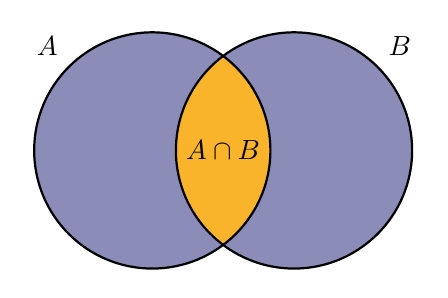
\begin{tikzpicture}[thick, set/.style = {circle, minimum size = 3cm, fill=MidnightBlue!50}]
		\node[set,label={135:$A$}] (A) at (0,0) {};
		\node[set,label={45:$B$}] (B) at (1.8,0) {};

		\begin{scope}
			\clip (0,0) circle(1.5cm);
			\clip (1.8,0) circle(1.5cm);
			\fill[Dandelion](0,0) circle(1.5cm);
		\end{scope}

		\draw (0,0) circle(1.5cm);
		\draw (1.8,0) circle(1.5cm);
		\node at (0.9,0) {$ A \cap B $};
	\end{tikzpicture}
	\caption{交集}
\end{figure}

如果两个集合没有公共元素,那么它们的交集为空集。\\

\subsection{并集(Union)}

假设$ A $和$ B $是两个集合,由它们所有元素合并在一起组成的集合,称为$ A $与$ B $的并集,表示为$ A \cup B $。

\begin{figure}[H]
	\centering
	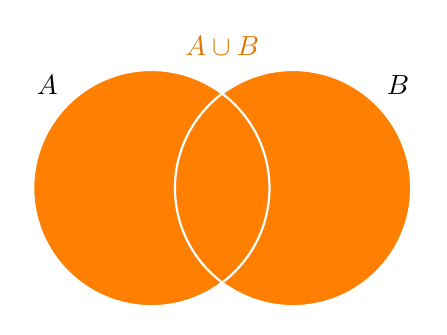
\begin{tikzpicture}
		\node [circle, fill=orange, minimum size=3cm, label={135:$A$}] (A) at (0,0){};
		\node [circle,
			fill=orange,
			minimum size =3cm,
			label={45:$B$}] (B) at (1.8,0){};

		\draw[white,thick] (0,0) circle(1.5cm);
		\draw[white,thick] (1.8,0) circle(1.5cm);
		\node[orange!90!black] at (0.9,1.8) {$ A \cup B $};
	\end{tikzpicture}
	\caption{并集}
\end{figure}

\vspace{0.5cm}

\subsection{差集(Difference)}

假设$ A $和$ B $是两个集合,由属于$ A $而不属于$ B $的元素组成的集合,称为$ A $与$ B $的差集,表示为$ A - B $。\\

差集运算不满足交换律,即$ A - B \neq B - A $。

\begin{figure}[H]
	\centering
	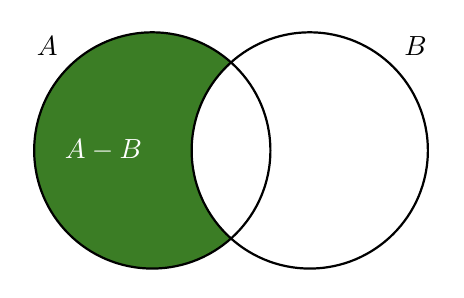
\begin{tikzpicture}[thick, set/.style = { circle, minimum size = 3cm}]
		\node[set,fill=OliveGreen,label={135:$A$}] (A) at (0,0) {};
		\node[set,fill=white,label={45:$B$}] (B) at (0:2) {};

		\draw (0,0) circle(1.5cm);
		\draw (2,0) circle(1.5cm);
		\node[left,white] at (A.center){$ A - B $};
	\end{tikzpicture}
	\caption{差集$ A - B $}
\end{figure}

\begin{figure}[H]
	\centering
	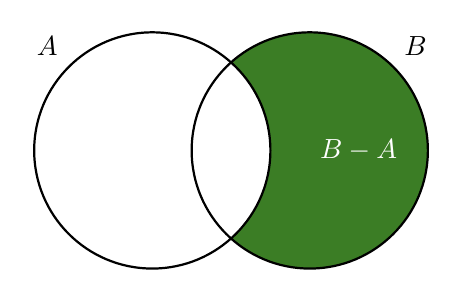
\begin{tikzpicture}[thick, set/.style = { circle, minimum size = 3cm}]
		\node[set,fill=OliveGreen,label={45:$B$}] (B) at (0:2) {};
		\node[set,fill=white,label={135:$A$}] (A) at (0,0) {};

		\draw (0,0) circle(1.5cm);
		\draw (2,0) circle(1.5cm);

		\node[right,white] at (B.center){$ B - A $};
	\end{tikzpicture}
	\caption{差集$ B - A $}
\end{figure}

\newpage

\section{集合恒等式}

\subsection{集合恒等式}

集合恒等式可以直接由对应的逻辑等价式证明。

\begin{tcolorbox}
	\mybox{幂等律 Idempotent Laws}
	\begin{align}
		A \cap A = A \\
		A \cup A = A
	\end{align}
\end{tcolorbox}

\begin{tcolorbox}
	\mybox{恒等律 Identity Laws}
	\begin{align}
		A \cap U = A \\
		A \cup \emptyset = A
	\end{align}
\end{tcolorbox}

\begin{tcolorbox}
	\mybox{支配律 Domination Laws}
	\begin{align}
		A \cap \emptyset = \emptyset \\
		A \cup U = U
	\end{align}
\end{tcolorbox}

\begin{tcolorbox}
	\mybox{双非律 Double Negation Law}
	\begin{align}
		\overline {\overline A} = A
	\end{align}
\end{tcolorbox}

\begin{tcolorbox}
	\mybox{交换律 Commutative Laws}
	\begin{align}
		A \cap B = B \cap A \\
		A \cup B = B \cup A
	\end{align}
\end{tcolorbox}

\begin{tcolorbox}
	\mybox{结合律 Associative Laws}
	\begin{align}
		(A \cap B) \cap C = A \cap (B \cap C) \\
		(A \cup B) \cup C = A \cup (B \cup C)
	\end{align}
\end{tcolorbox}

\begin{tcolorbox}
	\mybox{分配律 Distributive Laws}
	\begin{align}
		A \cap (B \cup C) = (A \cap B) \cup (A \cap C) \\
		A \cup (B \cap C) = (A \cup B) \cap (A \cup C)
	\end{align}
\end{tcolorbox}

\begin{tcolorbox}
	\mybox{德摩根律 De Morgan's Laws}
	\begin{align}
		\overline{A \cap B} = \overline A \cup \overline B
	\end{align}
\end{tcolorbox}

\begin{tcolorbox}
	\mybox{吸收律 Absorption Laws}
	\begin{align}
		A \cap (A \cup B) = A \\
		A \cup (A \cap B) = A
	\end{align}
\end{tcolorbox}

\begin{tcolorbox}
	\mybox{证明}
	$ \overline{A \cup (B \cap C)} = (\overline C \cup \overline B) \cap \overline A $
	\begin{align*}
		 & \overline{A \cup (B \cap C)}                      \\
		 & = \overline A \cap \overline{B \cap C}            \\
		 & = \overline A \cap (\overline B \cup \overline C) \\
		 & = (\overline B \cup \overline C) \cap \overline A \\
		 & = (\overline C \cup \overline B) \cap \overline A
	\end{align*}
\end{tcolorbox}

\begin{tcolorbox}
	\mybox{Exercise}
	一共有40个学生,有3门课程可供学生选择(C语言、离散数学、软件工程)。\\
	7人没有选任何课程;\\
	16人选软件工程;\\
	10人选C语言;\\
	5人同时选离散数学和软件工程;\\
	4人同时选离散数学和C语言;\\
	3人同时选软件工程和C语言;\\
	2人同时选离散数学、软件工程和C语言。\\

	\begin{figure}[H]
		\centering
		\begin{tikzpicture}
			\tikzset{venn circle/.style={draw,circle,minimum width=6cm,fill=#1,opacity=0.4}}
			\node [] () at (-2, -3) {C语言};
			\node [] () at (2, 7) {离散数学};
			\node [] () at (6, -3) {软件工程};
			\node [] () at (6, 7) {$ U $};
			\node [] () at (6, 6.5) {7};
			\node [venn circle = red] (A) at (0,0) {5};
			\node [venn circle = blue] (B) at (60:4cm) {10};
			\node [venn circle = green] (C) at (0:4cm) {10};
			\node[left] at (barycentric cs:A=1/2,B=1/2) {2};
			\node[below] at (barycentric cs:A=1/2,C=1/2) {1};
			\node[right] at (barycentric cs:B=1/2,C=1/2) {3};
			\node[below] at (barycentric cs:A=1/3,B=1/3,C=1/3) {2};
		\end{tikzpicture}
	\end{figure}
\end{tcolorbox}

\newpage

\section{笛卡尔积}

\subsection{元组(Tuple)}

有时候元素聚集中次序是很重要的,由于集合是无序的,所以就需要一种不同的结构表示有序的聚集,这就是有序$ n $元组(ordered-n-tuple)。\\

有序$ n $元组$ (a_1,\ a_2,\ \dots,\ a_n) $是以$ a_1 $为第$ 1 $个元素,$ a_2 $为第$ 2 $个元素,$ a_n $为第$ n $个元素的有序聚集。\\

只有两个有序$ n $元组的每一对对应的元素都相等,那么这两个有序$ n $元组是相等的,即:

\vspace{-0.5cm}

$$
	(a_1,\ a_2,\ \dots,\ a_n) = (b_1,\ b_2,\ \dots,\ b_n)\ \text{iff}\ i = 1,\ 2,\ \dots,\ n
$$

需要注意,$ (a,\ b) $与$ (b,\ a) $不相等,除非$ a = b $。\\

\subsection{笛卡尔积(Cartesian Product)}

假设有两个集合$ A $和$ B $,$ A $和$ B $的笛卡尔积用$ A \times B $表示,笛卡尔积是所有序偶$ (a,\ b) $的集合,其中$ a \in A $且$ b \in B $。

\vspace{-0.5cm}

$$
	A \times B = \{(a,\ b)\ |\ a \in A \wedge b \in B\}
$$

笛卡尔积$ A \times B $和$ B \times A $是不相等的,除非$ A = \emptyset $或$ B = \emptyset $或$ A = B $。

\begin{tcolorbox}
	\mybox{Exercise}
	笛卡尔积\\
	学生集合$ S = \{s1,\ s2\} $\\
	课程集合$ C = \{c1,\ c2,\ c3\} $\\
	$ S \times C = \{(s1,\ c1),\ (s1,\ c2),\ (s1,\ c3),\ (s2,\ c1),\ (s2,\ c2),\ (s2,\ c3)\} $\\
	笛卡尔积$ S \times C $表示学生选课的所有可能情况\\
\end{tcolorbox}

\begin{tcolorbox}
	\mybox{Exercise}
	笛卡尔积$ A \times B \times C $\\
	$ A = \{0,\ 1\} $\\
	$ B = \{1,\ 2\} $\\
	$ C = \{0,\ 1,\ 2\} $
	\begin{align*}
		A \times B \times C = \{(0, 1, 0), (0, 1, 1), (0, 1, 2), (0, 2, 0), (0, 2, 1), (0, 2, 2), \\
		(1, 1, 0), (1, 1, 1), (1, 1, 2), (1, 2, 0), (1, 2, 1), (1, 2, 2)\}
	\end{align*}
\end{tcolorbox}

一个集合与自身的笛卡尔积,如$ A \times A $可表示为$ A^2 $。

\begin{tcolorbox}
	\mybox{Exercise}
	笛卡尔积$ A^2 $\\
	$ A = \{1,\ 2\} $\\
	$ A^2 = \{(1,\ 1),\ (1,\ 2),\ (2,\ 1),\ (2,\ 2)\} $
\end{tcolorbox}

\newpage
\chapter{函数}

\section{函数}

\subsection{函数(Function)}

函数在数学和计算机科学中的概念非常重要,在离散数学中函数用于定义像序列和字符串这样的离散结构。\\

利用一个函数$ f $,可以将一个值$ x \in \mathbb{R} $映射(mapping)到一个特定的值$ y = f(x),\ y \in \mathbb{R} $ 上。\\

假设有两个非空集合$ X $和$ Y $,从$ X $到$ Y $的函数$ f $是指对于$ X $的每个元素恰好都对应$ Y $的一个元素,即$ f(x) = y,\ x \in X,\ y \in Y $,那么就写成$ f: X \rightarrow Y $。\\

集合$ X $被称为函数$ f $的定义域(domain),集合$ Y $被称为函数$ f $的陪域(co-domain)。\\

如果$ f(x) = y $,那么$ y $是$ x $在函数$ f $下的像(image),$ x $是$ y $在函数$ f $下的原像(pre-image)。函数$ f $的值域(range)是集合$ X $中所有像的集合。\\

当两个函数$ f $和$ g $有相同的定义域和陪域,并且对于定义域中所有元素$ x $都满足$ f(x) = g(x) $,那么函数$ f $和$ g $相等,表示为$ f = g $。

\begin{tcolorbox}
	\mybox{Exercise}
	判断是否为函数\\
	\begin{figure}[H]
		\centering
		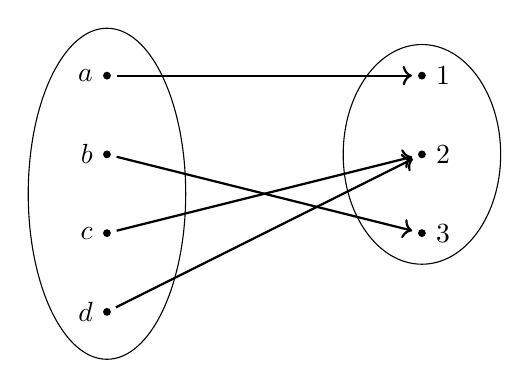
\begin{tikzpicture}[ele/.style={fill=black,circle,minimum width=.8pt,inner sep=1pt},every fit/.style={ellipse,draw,inner sep=-2pt}]
			\node[ele,label=left:$a$] (a) at (0,4) {};
			\node[ele,label=left:$b$] (b) at (0,3) {};
			\node[ele,label=left:$c$] (c) at (0,2) {};
			\node[ele,label=left:$d$] (d) at (0,1) {};

			\node[ele,,label=right:$1$] (v1) at (4,4) {};
			\node[ele,,label=right:$2$] (v2) at (4,3) {};
			\node[ele,,label=right:$3$] (v3) at (4,2) {};

			\node[draw,fit= (a) (b) (c) (d),minimum width=2cm] {} ;
			\node[draw,fit= (v1) (v2) (v3),minimum width=2cm] {} ;
			\draw[->,thick,shorten <=2pt,shorten >=2] (a) -- (v1);
			\draw[->,thick,shorten <=2pt,shorten >=2] (b) -- (v3);
			\draw[->,thick,shorten <=2pt,shorten >=2] (c) -- (v2);
			\draw[->,thick,shorten <=2pt,shorten >=2] (d) -- (v2);
		\end{tikzpicture}
		\caption{函数}
	\end{figure}

	\begin{figure}[H]
		\centering
		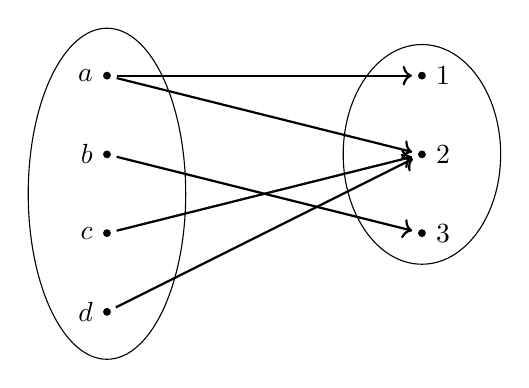
\begin{tikzpicture}[ele/.style={fill=black,circle,minimum width=.8pt,inner sep=1pt},every fit/.style={ellipse,draw,inner sep=-2pt}]
			\node[ele,label=left:$a$] (a) at (0,4) {};
			\node[ele,label=left:$b$] (b) at (0,3) {};
			\node[ele,label=left:$c$] (c) at (0,2) {};
			\node[ele,label=left:$d$] (d) at (0,1) {};

			\node[ele,,label=right:$1$] (v1) at (4,4) {};
			\node[ele,,label=right:$2$] (v2) at (4,3) {};
			\node[ele,,label=right:$3$] (v3) at (4,2) {};

			\node[draw,fit= (a) (b) (c) (d),minimum width=2cm] {} ;
			\node[draw,fit= (v1) (v2) (v3),minimum width=2cm] {} ;
			\draw[->,thick,shorten <=2pt,shorten >=2] (a) -- (v1);
			\draw[->,thick,shorten <=2pt,shorten >=2] (a) -- (v2);
			\draw[->,thick,shorten <=2pt,shorten >=2] (b) -- (v3);
			\draw[->,thick,shorten <=2pt,shorten >=2] (c) -- (v2);
			\draw[->,thick,shorten <=2pt,shorten >=2] (d) -- (v2);
		\end{tikzpicture}
		\caption{非函数}
	\end{figure}
\end{tcolorbox}

\begin{tcolorbox}
	\mybox{Exercise}
	\begin{figure}[H]
		\centering
		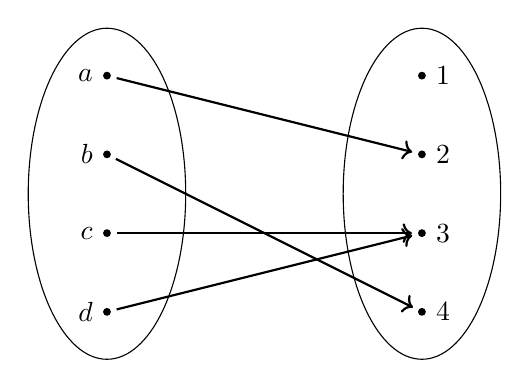
\begin{tikzpicture}[ele/.style={fill=black,circle,minimum width=.8pt,inner sep=1pt},every fit/.style={ellipse,draw,inner sep=-2pt}]
			\node[ele,label=left:$a$] (a) at (0,4) {};
			\node[ele,label=left:$b$] (b) at (0,3) {};
			\node[ele,label=left:$c$] (c) at (0,2) {};
			\node[ele,label=left:$d$] (d) at (0,1) {};

			\node[ele,,label=right:$1$] (v1) at (4,4) {};
			\node[ele,,label=right:$2$] (v2) at (4,3) {};
			\node[ele,,label=right:$3$] (v3) at (4,2) {};
			\node[ele,,label=right:$4$] (v4) at (4,1) {};

			\node[draw,fit= (a) (b) (c) (d),minimum width=2cm] {} ;
			\node[draw,fit= (v1) (v2) (v3) (v4),minimum width=2cm] {} ;
			\draw[->,thick,shorten <=2pt,shorten >=2] (a) -- (v2);
			\draw[->,thick,shorten <=2pt,shorten >=2] (b) -- (v4);
			\draw[->,thick,shorten <=2pt,shorten >=2] (c) -- (v3);
			\draw[->,thick,shorten <=2pt,shorten >=2] (d) -- (v3);
		\end{tikzpicture}
	\end{figure}

	是否为函数:是\\
	定义域(domain):$ a,\ b,\ c,\ d $\\
	陪域(co-domain):$ 1,\ 2,\ 3,\ 4 $\\
	值域(range):$ 2,\ 3,\ 4 $
\end{tcolorbox}

\newpage

\section{取整函数}

\subsection{上取整函数(Ceiling Function)}

取整函数包括上取整和下取整,可以将实数映射到整数($ \mathbb{R} \rightarrow \mathbb{Z} $),它们以不同的方式将实数近似到相邻的整数。\\

上取整函数将实数$ x $向上取到大于或等于$ x $的最小整数,表示为$ \lceil x \rceil $。

\begin{tcolorbox}
	\mybox{Exercise}
	上取整函数\\
	$ \lceil 3.2 \rceil = 4 $\\
	$ \lceil 2.6 \rceil = 3 $\\
	$ \lceil -0.5 \rceil = 0 $
\end{tcolorbox}

\vspace{0.5cm}

\subsection{下取整函数(Floor Function)}

下取整函数将实数$ x $向下取到小于或等于$ x $的最大整数,表示为$ \lfloor x \rfloor $。

\begin{tcolorbox}
	\mybox{Exercise}
	下取整函数\\
	$ \lfloor 3.2 \rfloor = 3 $\\
	$ \lfloor 5.9 \rfloor = 5 $\\
	$ \lfloor -0.5 \rfloor = -1 $
\end{tcolorbox}

\newpage

\section{函数分类}

\subsection{一对一函数(One-to-one) / 单射函数(Injection)}

一对一函数 / 单射函数是指对于函数$ f $的定义域中所有的$ a $和$ b $,如果$ a \neq b $,那么$ f(a) \neq f(b) $。

\begin{figure}[H]
	\centering
	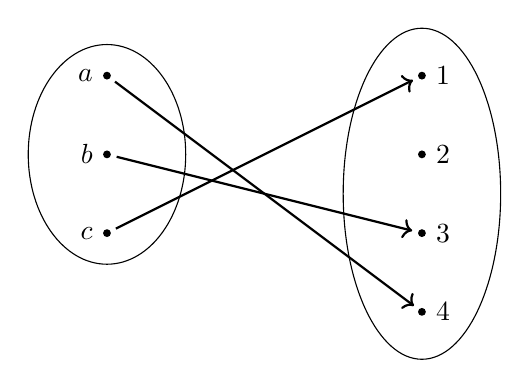
\begin{tikzpicture}[ele/.style={fill=black,circle,minimum width=.8pt,inner sep=1pt},every fit/.style={ellipse,draw,inner sep=-2pt}]
		\node[ele,label=left:$a$] (a) at (0,4) {};
		\node[ele,label=left:$b$] (b) at (0,3) {};
		\node[ele,label=left:$c$] (c) at (0,2) {};

		\node[ele,,label=right:$1$] (v1) at (4,4) {};
		\node[ele,,label=right:$2$] (v2) at (4,3) {};
		\node[ele,,label=right:$3$] (v3) at (4,2) {};
		\node[ele,,label=right:$4$] (v4) at (4,1) {};

		\node[draw,fit= (a) (b) (c),minimum width=2cm] {} ;
		\node[draw,fit= (v1) (v2) (v3) (v4),minimum width=2cm] {} ;
		\draw[->,thick,shorten <=2pt,shorten >=2] (a) -- (v4);
		\draw[->,thick,shorten <=2pt,shorten >=2] (b) -- (v3);
		\draw[->,thick,shorten <=2pt,shorten >=2] (c) -- (v1);
	\end{tikzpicture}
	\caption{一对一函数 / 单射函数}
\end{figure}

\begin{tcolorbox}
	\mybox{Exercise}
	一对一函数 / 单射函数\\
	$ f(x) = x + 1 $是一对一函数。\\
	$ f(x) = x^2 $不是一对一函数,因为$ f(1) = f(-1) = 1 $。
\end{tcolorbox}

\vspace{0.5cm}

\subsection{映上函数(Onto) / 满射函数(Surjection)}

映上函数 / 满射函数是指对于函数$ f: A \rightarrow B $,每个$ b \in B $都有元素$ a \in A $使得$ f(a) = b $。

\begin{figure}[H]
	\centering
	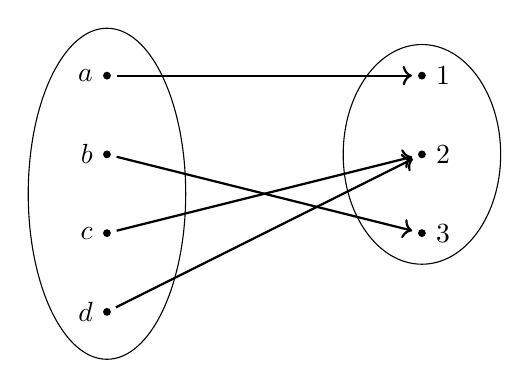
\begin{tikzpicture}[ele/.style={fill=black,circle,minimum width=.8pt,inner sep=1pt},every fit/.style={ellipse,draw,inner sep=-2pt}]
		\node[ele,label=left:$a$] (a) at (0,4) {};
		\node[ele,label=left:$b$] (b) at (0,3) {};
		\node[ele,label=left:$c$] (c) at (0,2) {};
		\node[ele,label=left:$d$] (d) at (0,1) {};

		\node[ele,,label=right:$1$] (v1) at (4,4) {};
		\node[ele,,label=right:$2$] (v2) at (4,3) {};
		\node[ele,,label=right:$3$] (v3) at (4,2) {};

		\node[draw,fit= (a) (b) (c) (d),minimum width=2cm] {} ;
		\node[draw,fit= (v1) (v2) (v3),minimum width=2cm] {} ;
		\draw[->,thick,shorten <=2pt,shorten >=2] (a) -- (v1);
		\draw[->,thick,shorten <=2pt,shorten >=2] (b) -- (v3);
		\draw[->,thick,shorten <=2pt,shorten >=2] (c) -- (v2);
		\draw[->,thick,shorten <=2pt,shorten >=2] (d) -- (v2);
	\end{tikzpicture}
	\caption{映上函数 / 满射函数}
\end{figure}

\begin{tcolorbox}
	\mybox{Exercise}
	映上函数 / 满射函数\\
	$ f: \mathbb{Z} \rightarrow \mathbb{Z},\ f(x) = x + 1 $是映上函数。\\
	$ f: \mathbb{Z} \rightarrow \mathbb{Z},\ f(x) = x^2 $不是映上函数,因为没有整数$ x $使$ x^2 = -1 $。
\end{tcolorbox}

\vspace{0.5cm}

\subsection{一一对应函数 / 双射函数(Bijection)}

如果一个函数既是一对一函数又是映上函数,那么这个函数就被称为一一对应函数 / 双射函数。

\begin{figure}[H]
	\centering
	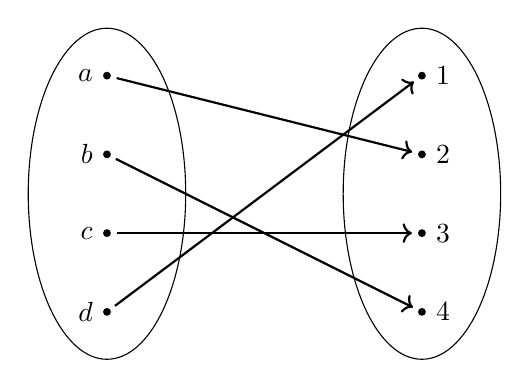
\begin{tikzpicture}[ele/.style={fill=black,circle,minimum width=.8pt,inner sep=1pt},every fit/.style={ellipse,draw,inner sep=-2pt}]
		\node[ele,label=left:$a$] (a) at (0,4) {};
		\node[ele,label=left:$b$] (b) at (0,3) {};
		\node[ele,label=left:$c$] (c) at (0,2) {};
		\node[ele,label=left:$d$] (d) at (0,1) {};

		\node[ele,,label=right:$1$] (v1) at (4,4) {};
		\node[ele,,label=right:$2$] (v2) at (4,3) {};
		\node[ele,,label=right:$3$] (v3) at (4,2) {};
		\node[ele,,label=right:$4$] (v4) at (4,1) {};

		\node[draw,fit= (a) (b) (c) (d),minimum width=2cm] {} ;
		\node[draw,fit= (v1) (v2) (v3) (v4),minimum width=2cm] {} ;
		\draw[->,thick,shorten <=2pt,shorten >=2] (a) -- (v2);
		\draw[->,thick,shorten <=2pt,shorten >=2] (b) -- (v4);
		\draw[->,thick,shorten <=2pt,shorten >=2] (c) -- (v3);
		\draw[->,thick,shorten <=2pt,shorten >=2] (d) -- (v1);
	\end{tikzpicture}
	\caption{一一对应函数 / 双射函数}
\end{figure}

\begin{tcolorbox}
	\mybox{Exercise}
	一一对应函数 / 双射函数\\
	$ f $是从$ \{a,\ b,\ c,\ d\} $到$ \{1,\ 2,\ 3,\ 4\} $的函数,定义$ f(a) = 4,\ f(b) = 2,\ f(c) = 1,\ f(d) = 3 $。\\
	函数$ f $是单射函数,因为没有两个值映射到相同的函数值。\\
	函数$ f $是满射函数,因为陪域的个数与值域的个数相同。\\
	因此,函数$ f $是双射函数。
\end{tcolorbox}

\newpage

\section{反函数}

\subsection{反函数(Inverse Function)}

假设有一个从集合$ A $到集合$ B $的双射函数$ f $。由于$ f $是满射函数,所以$ B $中的每个元素都是$ A $中某些元素的像;又由于$ f $还是单射函数,所以$ B $的每个元素都是$ A $中唯一一个元素的像。\\

于是,通过把f的对应关系颠倒,获得的从$ B $到$ A $的新函数被称为$ f $的反函数,用$ f^{-1} $表示。当$ f(a) = b $时,$ f^{-1}(b) = a $。需要注意,不要将$ f^{-1} $与$ 1 \over f $混淆。

\begin{tcolorbox}
	\mybox{Exercise}
	反函数
	\begin{figure}[H]
		\centering
		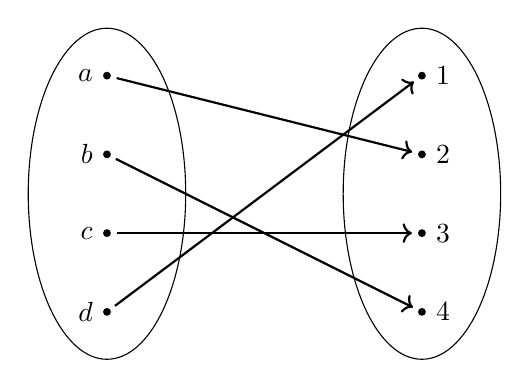
\begin{tikzpicture}[ele/.style={fill=black,circle,minimum width=.8pt,inner sep=1pt},every fit/.style={ellipse,draw,inner sep=-2pt}]
			\node[ele,label=left:$a$] (a) at (0,4) {};
			\node[ele,label=left:$b$] (b) at (0,3) {};
			\node[ele,label=left:$c$] (c) at (0,2) {};
			\node[ele,label=left:$d$] (d) at (0,1) {};

			\node[ele,,label=right:$1$] (v1) at (4,4) {};
			\node[ele,,label=right:$2$] (v2) at (4,3) {};
			\node[ele,,label=right:$3$] (v3) at (4,2) {};
			\node[ele,,label=right:$4$] (v4) at (4,1) {};

			\node[draw,fit= (a) (b) (c) (d),minimum width=2cm] {} ;
			\node[draw,fit= (v1) (v2) (v3) (v4),minimum width=2cm] {} ;
			\draw[->,thick,shorten <=2pt,shorten >=2] (a) -- (v2);
			\draw[->,thick,shorten <=2pt,shorten >=2] (b) -- (v4);
			\draw[->,thick,shorten <=2pt,shorten >=2] (c) -- (v3);
			\draw[->,thick,shorten <=2pt,shorten >=2] (d) -- (v1);
		\end{tikzpicture}
	\end{figure}
	是否有反函数:是\\
	$ f^{-1}(2) = a $\\
	$ f^{-1}(1) = 1 $
\end{tcolorbox}

\begin{tcolorbox}
	\mybox{Exercise}
	计算$ f(x) = x + 3 $的反函数\\
	$ f^{-1}(x) = x - 3 $
\end{tcolorbox}

\newpage

\section{合成函数}

\subsection{合成函数(Composition Function)}

假设$ g $是从集合$ A $到集合$ B $的函数,$ f $是从集合$ B $到集合$ C $的函数。函数$ f $和$ g $的合成,记作$ f \circ g $。

\vspace{-0.5cm}

$$
	(f \circ g)(x) = f(g(x))
$$

函数合成的顺序很重要,$ f \circ g $与$ g \circ f $并不相等。

\begin{tcolorbox}
	\mybox{Exercise}
	合成函数\\
	$ f: \mathbb{R^+} \rightarrow \mathbb{R^+},\ f(x) = x^3 $\\
	$ g: \mathbb{R^+} \rightarrow \mathbb{R^+},\ g(x) = x + 2 $\\
	$ (f \circ g)(x) = f(g(x)) = (x + 2)^3 $\\
	$ (g \circ f)(x) = g(f(x)) = x^3 + 2 $
\end{tcolorbox}

\vspace{0.5cm}

\subsection{恒等函数(Identity Function)}

如果一个从集合$ A $到集合$ B $的函数$ f $有反函数,那么$ f $与$ f^{-1} $的合成函数得到的是恒等函数。\\

如果$ f(a) = b $,那么$ f^{-1}(b) = a $。

\vspace{-0.5cm}

$$
	(f \circ f^{-1})(a) = f^{-1}(f(a)) = f^{-1}(b) = a
$$

\newpage

\section{指数函数与对数函数}

\subsection{指数函数(Exponential Function)}

指数函数的定义为$ y = a^x\ (a > 0\ |\ a \neq 1) $,其中$ a $称为底数(base),$ x $称为指数(exponent)。

\begin{figure}[H]
	\centering
	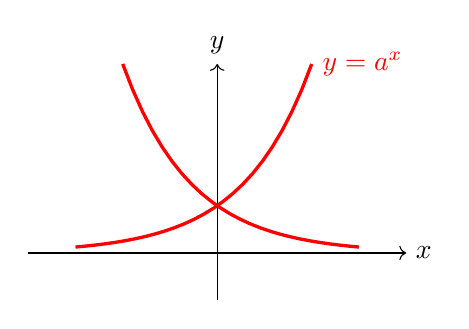
\begin{tikzpicture}[scale=0.6]
		\draw[->] (-4,0) -- (4,0) node[right] {$ x $};
		\draw[->] (0,-1) -- (0,4) node[above] {$ y $};
		\draw[very thick,color=red,domain=-3:2] plot (\x,{2 ^ \x}) node[right] {$ y = {a^x} $};
		\draw[very thick,color=red,domain=-2:3] plot (\x,{0.5 ^ \x});
	\end{tikzpicture}
	\caption{指数函数}
\end{figure}

\begin{tcolorbox}
	\mybox{指数函数}
	\begin{align}
		 & a^{-x} = {1 \over a^x}                    \\
		 & {1 \over a^{-x}} = a^x                    \\
		 & (ab)^x = a^xb^x                           \\
		 & ({a \over b})^x = {a^x \over b^x}         \\
		 & a^{kx} = (a^k)^x = (a^x)^k                \\
		 & a^ma^n = a^{m+n}                          \\
		 & {a^m \over a^n} = a^{m-n}                 \\
		 & a^{1/n} = \sqrt[n]{a}                     \\
		 & a^{m/n} = \sqrt[n]{a^m} = (\sqrt[n]{a})^m
	\end{align}
\end{tcolorbox}

\begin{tcolorbox}
	\mybox{Exercise}
	指数函数\\
	$ (6^{2k})^3 = 6^{6k} $\\
	$ 6^{k^2} \times 6 = 6^{k^2 + 1} $\\
	$ {3^k \over 9} = {3^k \over 3^2} = 3^{k-2} $\\
	$ 3^k \times 27 = 3^k \times 3^3 = 3^{k+3} $
\end{tcolorbox}

\vspace{0.5cm}

\subsection{对数函数(Logarithm Function)}

对于函数$ f: \{1,\ 2,\ 3,\ 4\} \rightarrow \{1,\ 4,\ 8,\ 16\},\ f(x) = 2^x $,指数函数是双射函数,因此它是有反函数的。\\

对数函数是指数函数的反函数,对数函数的定义为$ y = log_a{x}\ (a > 0\ |\ a \neq 1) $,其中$ a $称为底数。

\begin{figure}[H]
	\centering
	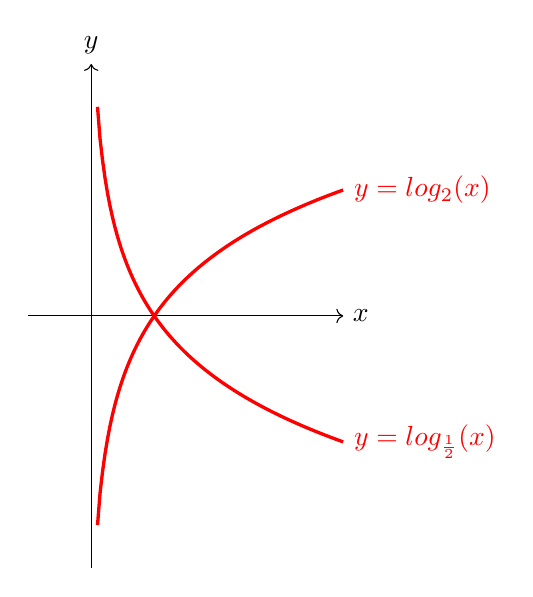
\begin{tikzpicture}[scale=0.8]
		\draw[->] (-1,0) -- (4,0) node[right] {$ x $};
		\draw[->] (0,-4) -- (0,4) node[above] {$ y $};
		\draw [very thick,color=red,domain=0.1:4,samples=100] plot (\x,{log2(\x)}) node[right] {$ y = log_2(x) $};
		\draw [very thick,color=red,domain=0.1:4,samples=100] plot (\x,{log10(\x) / log10(0.5)}) node[right] {$ y = log_{1 \over 2}(x) $};
	\end{tikzpicture}
	\caption{对数函数}
\end{figure}

\begin{tcolorbox}
	\mybox{对数函数}
	\begin{align}
		 & log_a(a^x) = x                                      \\
		 & a^{log_a(x)} = x                                    \\
		 & log_a(xy) = log_a(x) + log_a(y)                     \\
		 & log_a\left({x \over y}\right) = log_a(x) - log_a(y) \\
		 & log_a(x^n) = nlog_a(x)                              \\
		 & log_a(x) = {log_b(x) \over log_b(a)}
	\end{align}
\end{tcolorbox}

\begin{tcolorbox}
	\mybox{Exercise}
	对数函数\\
	$ log_5{k} + log_5{2} = log_5{2k} $\\
	$ log_2{5^2} = 2 \times log_2{5} $\\
	$ {log_3{k^2} \over log_3{25}} = {2 \times log_3{k} \over log_3{5^2}} = {2 \times log_3{k} \over 2 \times log_3{5}} = log_5{k} $
\end{tcolorbox}

\newpage
\chapter{数论}

\section{进制转换}

\subsection{进制}

日常生活中都用十进制(decimal)来表示整数,十进制数由$ 0,\ 1,\ 2,\ 3,\ 4,\ 5,\ 6,\ 7,\ 8,\ 9 $这10个字符组成。一个十进制整数的第$ k $位的值可以由$ 10^{k-1} $计算得到。

\begin{tcolorbox}
	\mybox{Exercise}
	十进制
	\begin{align*}
		256 & = 200 + 50 + 6                                  \\
		    & = 2 \times 10^2 + 5 \times 10^1 + 6 \times 10^0
	\end{align*}
\end{tcolorbox}

二进制(binary)、八进制(octal)、十六进制(hexadecimal)也是非常常用的表示法,例如计算机通常用二进制来做算术运算,而用八进制或十六进制来表示字符。\\

\subsection{进制转换}

一个$ b $进制的正整数$ n $可以唯一地构造展开式:

\vspace{-0.5cm}

$$
	n = a^k \times b^k + a_{k-1} \times b^{k-1} + \dots + a_1 \times b^1 + a_0 \times b^0
$$

\begin{tcolorbox}
	\mybox{Exercise}
	$ b $进制转十进制\\
	$ (1011)_2 = 1 \times 2^3 + 0 \times 2^2 + 1 \times 2^1 + 1 \times 2^0 = (11)_{10} $\\
	$ (21022)_3 = 2 \times 3^4 + 1 \times 3^3 + 0 \times 3^2 + 2 \times 3^1 + 2 \times 3^0 = (197)_{10} $
\end{tcolorbox}

\begin{table}[H]
	\centering
	\setlength{\tabcolsep}{5mm}{
		\begin{tabular}{|c|c|c|c|}
			\hline
			\textbf{十进制} & \textbf{二进制} & \textbf{八进制} & \textbf{十六进制} \\
			\hline
			0               & 0               & 0               & 0                 \\
			\hline
			1               & 1               & 1               & 1                 \\
			\hline
			2               & 10              & 2               & 2                 \\
			\hline
			3               & 11              & 3               & 3                 \\
			\hline
			4               & 100             & 4               & 4                 \\
			\hline
			5               & 101             & 5               & 5                 \\
			\hline
			6               & 110             & 6               & 6                 \\
			\hline
			7               & 111             & 7               & 7                 \\
			\hline
			8               & 1000            & 10              & 8                 \\
			\hline
			9               & 1001            & 11              & 9                 \\
			\hline
			10              & 1010            & 12              & A                 \\
			\hline
			11              & 1011            & 13              & B                 \\
			\hline
			12              & 1100            & 14              & C                 \\
			\hline
			13              & 1101            & 15              & D                 \\
			\hline
			14              & 1110            & 16              & E                 \\
			\hline
			15              & 1111            & 17              & F                 \\
			\hline
		\end{tabular}
	}
	\caption{进制转换}
\end{table}

十进制转$ b $进制还可以使用短除法的方式。

\begin{tcolorbox}
	\mybox{Exercise}
	十进制转四进制\\
	\begin{tabular}{rl}
		4\mydiv{637} & remainder 1 \\
		4\mydiv{159} & remainder 3 \\
		4\mydiv{39}  & remainder 3 \\
		4\mydiv{9}   & remainder 1 \\
		4\mydiv{2}   & remainder 2
	\end{tabular}
	$ (637)_{10} = (21331)_4 $
\end{tcolorbox}

\begin{tcolorbox}
	\mybox{Exercise}
	十进制转二进制\\
	\begin{tabular}{rl}
		2\mydiv{637} & remainder 1 \\
		2\mydiv{318} & remainder 0 \\
		2\mydiv{159} & remainder 1 \\
		2\mydiv{79}  & remainder 1 \\
		2\mydiv{39}  & remainder 1 \\
		2\mydiv{19}  & remainder 1 \\
		2\mydiv{9}   & remainder 1 \\
		2\mydiv{4}   & remainder 0 \\
		2\mydiv{2}   & remainder 0 \\
		2\mydiv{1}   & remainder 1
	\end{tabular}
	$ (637)_{10} = (1001111101)_2 $
\end{tcolorbox}

\begin{tcolorbox}
	\mybox{Exercise}
	十进制转八进制\\
	\begin{tabular}{rl}
		8\mydiv{1000} & remainder 0 \\
		8\mydiv{125}  & remainder 5 \\
		8\mydiv{15}   & remainder 7 \\
		8\mydiv{1}    & remainder 1
	\end{tabular}
	$ (1000)_{10} = (1750)_8 $
\end{tcolorbox}

\newpage

\section{素数}

\subsection{素数(Prime Numbers)}

基于整除性的一个重要概念就是素数,素数是大于1的且不能被1和它自身以外的正整数整除的整数。素数是现代密码学中必不可少的一部分,密码学中的大素数就用在信息加密的某些方法中。

\begin{tcolorbox}
	\mybox{Exercise}
	判断素数\\
	7是素数,因子有1和7。\\
	9是合数,因为9能被3整除。
\end{tcolorbox}

每个大于1的整数都可以唯一地写成多个素数的乘积。

\begin{tcolorbox}
	\mybox{Exercise}
	素因子分解\\
	$ 100 = 2 \times 2 \times 5 \times 5 = 2^2 \times 5^2 $\\
	$ 999 = 3 \times 3 \times 3 \times 37 = 3^3 \times 37 $\\
	$ 1024 = 2^{10} $
\end{tcolorbox}

如果$ n $是一个合数,那么$ n $必有一个素因子小于或等于$ \sqrt{n} $。

\begin{tcolorbox}
	\mybox{Exercise}
	证明101是素数\\
	不超过$ \sqrt{101} $的素数只有$ 2, 3, 5, 7 $,因为$ 101 $不能被$ 2, 3, 5, 7 $整除,所以$ 101 $是素数。
\end{tcolorbox}

\vspace{-0.5cm}
\begin{lstlisting}[language=Python]
import math

def is_prime(num):
	for i in range(2, int(math.sqrt(num)) + 1):
		if num % i == 0:
			return False
	return True

def main():
	print(is_prime(13))
	print(is_prime(18))

if __name__ == "__main__":
	main()
\end{lstlisting}

埃拉托斯特尼筛法(Sieve of Eratosthenes)可以用来寻找不超过一个给定整数的所有素数。\\

步骤:

\begin{enumerate}
	\item 建立包含所有给定整数以内的表格
	\item 从$ i = 2 $开始
	\item 移除所有整数$ n \% i == 0 $(除$ i $以外)
	\item $ i = i + 1 $
	\item 重复第3步和第4步
\end{enumerate}

\begin{table}[H]
	\centering
	\setlength{\tabcolsep}{5mm}{
		\begin{tabular}{|c|c|c|c|c|c|c|c|c|c|}
			\hline
			   & 2  & 3  & 4  & 5  & 6  & 7  & 8  & 9  & 10 \\
			\hline
			11 & 12 & 13 & 14 & 15 & 16 & 17 & 18 & 19 & 20 \\
			\hline
			21 & 22 & 23 & 24 & 25 & 26 & 27 & 28 & 29 & 30 \\
			\hline
		\end{tabular}
	}
	\caption{埃拉托斯特尼筛法}
\end{table}

\newpage

\section{序列}

\subsection{序列(Sequence)}

序列是一种用来表示有序列表的离散结构。例如$ 1,\ 2,\ 3,\ 5,\ 8 $是一个含有五项的序列,而$ 1,\ 3,\ 9,\ 27,\ 81,\ \dots $是一个无穷序列。序列可以用记号$ \{a_n\} $表示。

\begin{itemize}
	\item 递增序列(increasing sequence): 一个序列任意相邻的两项满足$ a_k < a_{k+1} $
	\item 非递减序列(non-decreasing sequence): 一个序列任意相邻的两项满足$ a_k \le a_{k+1} $
	\item 递减序列(decreasing sequence): 一个序列任意相邻的两项满足$ a_k > a_{k+1} $
	\item 非递增序列(non-increasing sequence): 一个序列任意相邻的两项满足$ a_k \ge a_{k+1} $
\end{itemize}

\begin{tcolorbox}
	\mybox{Exercise}
	序列\\
	$ \{a_n\},\ a_n = {1 \over n}:\ 1,\ {1 \over 2},\ {1 \over 3},\ {1 \over 4},\ \dots $\\
	$ \{b_n\},\ b_n = 2^n:\ 1,\ 2,\ 4,\ 8,\ 16,\ 32,\ \dots $
\end{tcolorbox}

\vspace{0.5cm}

\subsection{算术级数(Arithmetic Sequence)}

算术级数也称等差级数,序列形式如下:

\vspace{-0.5cm}

$$
	a,\ a + d,\ a + 2d,\ \dots,\ a + nd,\ \dots\ (a, d \in \mathbb{R})
$$

\begin{tcolorbox}
	\mybox{Exercise}
	算术级数\\
	$ \{a_n\},\ a_n = -1 + 4n:\ -1,\ 3,\ 7,\ 11,\ \dots $\\
	$ \{b_n\},\ b_n = 7 - 3n:\ 7,\ 4,\ 1,\ -2,\ \dots $
\end{tcolorbox}

\vspace{0.5cm}

\subsection{几何级数(Geometric Sequence)}

几何级数也称等比级数,序列形式如下:

\vspace{-0.5cm}

$$
	a,\ ar,\ ar^2,\ \dots,\ ar^n,\ \dots,\ (a, r \in \mathbb{R})
$$

\begin{tcolorbox}
	\mybox{Exercise}
	几何级数\\
	$ \{a_n\},\ a_n = (-1)^n:\ 1,\ -1,\ 1,\ -1,\ 1,\ \dots $\\
	$ \{b_n\},\ b_n = -2 \times 5^n:\ 2,\ 10,\ 50,\ 250,\ 1250,\ \dots $\\
	$ \{c_n\},\ c_n = 6 \times ({1 \over 3})^n:\ 6,\ 2,\ {2 \over 3},\ {2 \over 9},\ {2 \over 27},\ \dots $
\end{tcolorbox}

\newpage

\section{递推关系}

\subsection{递推(Recurrence)}

如果数列$ \{a_n\} $的第$ n $项与它前一项的关系可以用一个公式来表示,那么这个公式就叫做这个数列的递推方程。\\

算术级数的递推关系:

\vspace{-1.5cm}

\begin{align*}
	a_0 & = a           \\
	a_n & = a_{n-1} + d
\end{align*}

几何级数的递推关系:

\vspace{-1.5cm}

\begin{align*}
	a_0 & = a                \\
	a_n & = a_{n-1} \times r
\end{align*}

\begin{tcolorbox}
	\mybox{Exercise}
	银行储蓄账户上有10000元,年利率为5.8\%,7年后账户中将有多少钱?
	\begin{align*}
		P_n & = P_{n-1} + 0.058P_{n-1}                      \\
		    & = (1.058)P_{n-1}                              \\
		\\
		P_0 & = 10000                                       \\
		P_1 & = (1.058)P_0                                  \\
		P_2 & = (1.058)P_1 = (1.058)^2 P_0                  \\
		\dots                                               \\
		P_7 & = (1.058)P_6 = (1.058)^7 P_0 \approx 14838.83
	\end{align*}
\end{tcolorbox}

\vspace{0.5cm}

\subsection{斐波那契数列(Fibonacci Sequence)}

斐波那契数列$ f_0,\ f_1,\ f_2,\ \dots $的递推公式为:

\begin{align*}
	f(n) = \begin{cases}
		1               & n = 1 \\
		1               & n = 2 \\
		f(n-1) + f(n-2) & n > 3
	\end{cases}
\end{align*}

斐波那契数列的通项公式为:

$$
	f_n = {1 \over \sqrt{5}} \left({1 + \sqrt{5} \over 2} \right)^{n+1} - {1 \over \sqrt{5}} \left({1 - \sqrt{5} \over 2} \right)^{n+1}
$$

\begin{lstlisting}[language=C, title=斐波那契数列(递归)]
int fibonacci(int n) {
	if(n == 1 || n == 2) {
		return 1;
	}
	return fibonacci(n-2) + fibonacci(n-1);
}
\end{lstlisting}

\begin{figure}[H]
	\centering
	\begin{tikzpicture}[
			level distance=2.5cm,
			level 1/.style={sibling distance=6cm},
			level 2/.style={sibling distance=3cm},
			level 3/.style={sibling distance=2cm}
		]
		\node {$ f(5) $}
		child {
				node {$ f(3) $}
				child {node {$ f(1) $}}
				child {
						node {$ f(2) $}
						child {node {$ f(0) $}}
						child {node {$ f(1) $}}
					}
			}
		child {
				node {$ f(4) $}
				child {
						node {$ f(2) $}
						child {node {$ f(0) $}}
						child {node {$ f(1) $}}
					}
				child {
						node {$ f(3) $}
						child {node {$ f(1) $}}
						child {
								node {$ f(2) $}
								child {node {$ f(0) $}}
								child {node {$ f(1) $}}
							}
					}
			};
	\end{tikzpicture}
	\caption{递归树}
\end{figure}

\begin{lstlisting}[language=C, title=斐波那契数列(迭代)]
int fibonacci(int n) {
	int f[n];
	f[0] = f[1] = 1;
	for(int i = 2; i < n; i++) {
		f[i] = f[i-2] + f[i-1];
	}
	return f[n-1];
}
\end{lstlisting}

\newpage

\section{求和}

\subsection{求和(Summation)}

求和符号$ \sum $可以用于表示序列中所有项的累加和。

$$
	\sum_{i=lower}^{upper} a_i
$$

\begin{tcolorbox}
	\mybox{Exercise}
	求和\\
	$ \sum_{i=1}^{100} i = 1 + 2 +3 + \dots + 99 + 100 = 5050 $\\
	$ \sum_{j=1}^{5} j^2 = 1^2 + 2^2 + 3^2 + 4^2 + 5^2 = 55 $\\
	$ \sum_{k=4}^{6} (-1)^k = (-1)^4 + (-1)^5 + (-1)^6 = 1 - 1 + 1 = 1 $
\end{tcolorbox}

\vspace{0.5cm}

\subsection{双重求和}

很多情况下需要使用双重求和,比如在计算机程序中嵌套循环的分析中。\\

计算双重求和的方法是先展开内层求和,再继续计算外层求和。

\begin{tcolorbox}
	\mybox{Exercise}
	双重求和
	\begin{align*}
		 & \sum_{i=1}^{4} \sum_{j=1}^{3} ij \\
		 & = \sum_{i=1}^{4} (i + 2i + 3i)   \\
		 & = \sum_{i=1}^{4} 6i              \\
		 & = 6 + 12 + 1 8 + 24              \\
		 & = 60
	\end{align*}
\end{tcolorbox}

\newpage

\section{数学归纳法}

\subsection{数学归纳法(Mathematical Induction)}

数学归纳法是一种数学证明方法,通常被用于证明某个给定命题在一个给定范围内成立。\\

数学归纳法分为三个步骤:

\begin{enumerate}
	\item 归纳基础
	\item 归纳假设
	\item 归纳递推
\end{enumerate}

\begin{tcolorbox}
	\mybox{证明}
	$ \sum_{i=1}^{n} i = {n(n+1) \over 2},\ n \in \mathbb{Z^+} $
	\begin{enumerate}
		\item 归纳基础:当$ n = 1 $,\\
		      $ \sum_{i=1}^{1} i = {1(1+1) \over 2} = 1 $

		\item 归纳假设:假设$ n = k $,\\
		      $ \sum_{i=1}^{k} i = {k(k+1) \over 2} $成立

		\item 归纳递推:证明$ n = k + 1 $时,
		      \begin{align*}
			      \sum_{i=1}^{k+1} i & = \sum_{i=1}^{k} i + k + 1  \\
			                         & = {k(k+1) \over 2} + k + 1  \\
			                         & = {k(k+1) + 2(k+1) \over 2} \\
			                         & = {(k+1)(k+2) \over 2}
		      \end{align*}
	\end{enumerate}
\end{tcolorbox}

\begin{tcolorbox}
	\mybox{证明}
	$ 2^n \ge 3n,\ n \ge 4 $
	\begin{enumerate}
		\item 归纳基础:当$ n = 4 $,\\
		      $ 2^4 \ge 3 \times 4 $

		\item 归纳假设:假设$ n = k\ (n > 4) $,\\
		      $ 2^k \ge 3k $成立

		\item 归纳递推:证明$ n = k + 1 $时,
		      \begin{align*}
			      2^{k+1} & = 2 \times 2^k  \\
			              & \ge 2 \times 3k \\
			              & = 3k + 3k       \\
			              & \ge 3k + 3      \\
			              & \ge 3(k+1)
		      \end{align*}
	\end{enumerate}
\end{tcolorbox}

\begin{tcolorbox}
	\mybox{证明}
	对于任意正整数n,3都能够整除$ 2^{2n} - 1 $
	\begin{enumerate}
		\item 归纳基础:当$ n = 1 $,\\
		      $ 2^{2 \times 1} -1 = 3 $

		\item 归纳假设:假设$ n = k\ (n > 0) $,\\
		      3能够整除$ 2^{2k} - 1 $成立,即$ 2^{2k} - 1 = 3m $

		\item 归纳递推:证明$ n = k + 1 $时,
		      \begin{align*}
			      2^{2(k+1)} - 1 & = 2^{2k+2} - 1          \\
			                     & = 4 \times 2^{2k} - 1   \\
			                     & = 4 \times (3m + 1) - 1 \\
			                     & = 4 \times 3m + 4 - 1   \\
			                     & =3 \times (4m + 1)
		      \end{align*}
	\end{enumerate}
\end{tcolorbox}

\newpage
\chapter{计数}

\section{计数}

\subsection{分类加法计数原理}

完成一件事有$ n $种不同的方案,其中第$ 1 $种方案有$ m_1 $种不同方法,第$ 2 $种方案有$ m_2 $种不同方法,$ \dots $,第$ n $种方案有$ m_n $种不同方法,那么完成这件事共有$ m_1 + m_2 + \dots + m_n $种不同方法。

\begin{tcolorbox}
	\mybox{Exercise}
	从A地到B地,可以乘火车、汽车、飞机。火车有4班、汽车2班、飞机3班,那么一天中乘坐这些交通工具从A地到B地有多少种不同的走法?
	$$
		4 + 2 + 3 = 9
	$$
\end{tcolorbox}

\vspace{0.5cm}

\subsection{分步乘法计数原理}

完成一件事需要$ n $个步骤,其中第$ 1 $个步骤有$ m_1 $种不同方法,第$ 2 $个步骤有$ m_2 $种不同方法,$ \dots $,第$ n $个步骤有$ m_n $种不同方法,那么完成这件事共有$ m_1 \times m_2 \times \dots m_n $种不同方法。

\begin{tcolorbox}
	\mybox{Exercise}
	一个书架的第1层有4本不同的计算机书,第2层有3本不同的经济书,第3层有2本不同的数学书。从书架的每一层各取一本书,有多少种不同取法?
	$$
		4 \times 3 \times 2 = 24
	$$
\end{tcolorbox}

\newpage

\section{排列}

\subsection{排列(Permutation)}

从$ n $个不同元素中取出$ m\ (m \le n) $ 个元素,按照一定次序排成一列,称为从$ n $个不同元素中取出$ m $个元素的一个排列。

\vspace{-1cm}

\begin{align}
	P_n^m = {n! \over (n-m)!}
\end{align}

例如一共有8个人,A、B、C、D、E、F、G、H。现在有3个奖杯,分别为金牌、银牌和铜牌。将这3个奖牌颁发给8个人中的3个,问颁发奖牌的不同方式总共有几种?\\

很明显这是一个排列的问题,因为把金牌先颁给A,再把银牌颁给B,跟把金牌先颁给B,再把银牌颁给A 这是两种不同的颁奖方式。

\begin{itemize}
	\item 第一步颁发金牌,金牌可以颁发给8个人中的1个,共有8种选择。

	\item 第二步颁发银牌,银牌可以颁发剩下7个人中的1个,共有7种选择。

	\item 第二步颁发铜牌,铜牌可以颁发剩下6个人中的1个,共有6种选择。
\end{itemize}

那么总共的颁奖方式共有$ 8 \times 7 \times 6 = 336 $种。

\begin{tcolorbox}
	\mybox{Exercise}
	用0-9这10个数字可以组成多少个没有重复数字的三位数?\\

	\textbf{方法一}\\
	由于0没有排在百位上,那么百位只能是1-9这9个数字任选1个,有$ P_9^1 $种选法。\\
	对于十位和个位,从余下的9个数字种选2个,有$ P_9^2 $种选法。
	$$
		P_9^1 \times P_9^2 = 9 \times 9 \times 8 = 648
	$$

	\textbf{方法二}\\
	符合条件的三位数可以分为3大类:
	\begin{enumerate}
		\item 每一位数字都不是0的三位数,也就是从1-9中选3个,有$ P_9^3 $种选法。

		\item 个位数字为0,那么需要从剩下9个数字中选2个作为十位和百位,有$ P_9^2 $种选法。

		\item 十位数字为0,那么需要从剩下9个数字中选2个作为个位和百位,有$ P_9^2 $种选法。
	\end{enumerate}
	$$
		P_9^3 + P_9^2 + P_9^2 = 648
	$$

	\textbf{方法三}\\
	利用容斥法。从0-9这10个数字任取3个数字的排列数为$ P_{10}^3 $,其中0在百位上(也就是从1-9中选2个作为十位和个位)的排列数是$ P_9^2 $。
	$$
		P_{10}^3 - P_9^2 = 648
	$$
\end{tcolorbox}

\begin{tcolorbox}
	\mybox{Exercise}
	打印字符串math的全排列。
\end{tcolorbox}

\begin{lstlisting}[language=C, title=全排列]
#include <stdio.h>
#include <string.h>

void swap(char *a, char *b) {
	char temp = *a;
	*a = *b;
	*b = temp;
}

void permutation(char *s, int start, int end) {
	if(start >= end) {
		printf("%s\n", s);
	} else {
		for(int i = start; i < end; i++) {
			swap(s + i, s + start);
			permutation(s, start + 1, end);
			swap(s + i, s + start);
		}
	}
}

int main() {
	char s[] = "math";
	int len = strlen(s);
	permutation(s, 0, len);
	return 0;
}
\end{lstlisting}

\newpage

\section{组合}

\subsection{组合(Combination)}

从$ n $个不同元素中取出$ m\ (m \le n) $ 个元素,称为从$ n $个不同元素中取出$ m $个元素的一个组合。\\

排列与组合的不同点在于,排列与元素的顺序有关,组合与元素的顺序无关。

\vspace{-1cm}

\begin{align}
	C_n^m = {P_n^m \over P_m^m} = {n! \over (n-m)!m!}
\end{align}

\begin{tcolorbox}
	\mybox{Exercise}
	在100件产品中,有98件合格品,2件次品,从这100件产品中任意抽出3件。\\
	(1) 有多少种不同的抽法?
	$$
		C_{100}^3 = {100 \times 99 \times 98 \over 3 \times 2 \times 1} = 161700
	$$

	(2) 抽出的3件中恰好有1件事次品的抽法有多少种?\\
	2件次品抽出1件有$ C_2^1 $种,再从98件合格品种抽出2件合格品有$ C_{98}^2 $种。
	$$
		C_2^1 \times C_{98}^2 = 9506
	$$

	(3) 抽出的3件中至少有1件事次品的抽法有多少种?\\
	\textbf{方法一}\\
	恰好有1件次品有$ C_2^1 \times C_{98}^2 $种,恰好有2件次品有$ C_2^2 \times C_{98}^1 $种。
	$$
		C_2^1 \times C_{98}^2 + C_2^2 \times C_{98}^1 = 9604
	$$

	\textbf{方法二}\\
	利用容斥法。先从100件抽出3件有$ C_{100}^3 $种,其中3件都是合格品有$ C_{98}^3 $种。
	$$
		C_{100}^3 - C_{98}^3 = 9604
	$$
\end{tcolorbox}

\newpage

\section{鸽巢原理}

\subsection{鸽巢原理(Pigeonhole Principle)}

鸽巢原理也称为狄利克雷抽屉原理(Dirichlet Drawer Principle),假设有20只鸽子要飞往19个鸽巢栖息,因此这19个鸽巢中至少有1个鸽巢最少栖息着2只鸽子。

\begin{tcolorbox}
	\mybox{鸽巢原理}\\
	如果k + 1个或者更多的物体放入k个盒子,那么至少有一个盒子包含了2个或更多的物体。
\end{tcolorbox}

在生活中有很多场景都可以用鸽巢原理来解释:

\begin{itemize}
	\item 367个人中一定至少有2个人生日相同。
	\item 27个英文单词中一定至少有2个单词是以同一个字母开头。
\end{itemize}

鸽巢原理指出当物体比盒子多时一定至少有2个物体在同一个盒子里,但是当物体树量超过盒子数量的倍数时,可以得到更多的结论。例如在21个在0 $ \sim $ 9数字中一定有3个是相同的,这是由于21个物体被分配到10个盒子里,那么某个盒子的物体一定多于2个。

\begin{tcolorbox}
	\mybox{广义鸽巢原理}\\
	如果N个物体放入k个盒子,那么至少有一个盒子包含了至少$ \lceil N / k \rceil $个物体。
\end{tcolorbox}

在生活中有很多场景都可以用广义鸽巢原理来解释:

\begin{itemize}
	\item 在100个人中至少有$ \lceil 100 / 12 \rceil = 9 $个人出生在同一个月。
	\item 假设有A、B、C、D、E五个成绩,一个班级至少要有26个学生才能保证至少6个学生得到相同的分数。
\end{itemize}

\begin{tcolorbox}
	\mybox{Exercise}
	(1) 从一副标准的52张牌中必须选多少张牌才能保证选出的牌中至少有3张是同样的花色?\\
	假设用4个盒子存放4种花色的牌,选N张牌后,至少有一个盒子含有至少$ \lceil N / 4 \rceil $张牌。\\
	因此使得$ \lceil N / 4 \rceil \ge 3 $的最小整数$ N = 2 \times 4 + 1 = 9 $\\

	(2) 必须选多少张牌才能保证选出的牌中至少有3张是红桃。\\
	这个场景不适用广义鸽巢原理,因为要保证存在3张红桃,而不是3张同花色的牌。\\
	最坏情况下,在选出第一张红桃之前已经选了所有的其它花色牌共39张,因此为了得到3张红桃,可能需要选42张牌。
\end{tcolorbox}

\newpage

\section{二项式定理}

\subsection{二项式系数(Binomial Coefficient)}

组合数$ C(n, r) $也可写为$ n \choose r $,由于这些数经常出现在$ (x + y)^n $的展开式中作为系数,所以这些数被称为二项式系数。

\vspace{-1cm}

\begin{align*}
	(x + y)^3 & = 1x^3 + 3x^2y + 3xy^2 + 1y^3                                                     \\
	          & = {3 \choose 0} x^3 + {3 \choose 1} x^2y + {3 \choose 2} xy^2 + {3 \choose 3} y^3
\end{align*}

\begin{tcolorbox}
	\mybox{二项式定理}
	\begin{align}
		(x + y)^n & = \sum_{j=0}^{n} {n \choose j}x^{n-j}y^j                                                            \\
		\nonumber
		          & = {n \choose 0} x^n + {n \choose 1} x^{n-1}y + \dots + {n \choose n-1} xy^{n-1} + {n \choose n} y^n
	\end{align}
\end{tcolorbox}

\begin{tcolorbox}
	\mybox{Exercise}
	计算$ (x + y)^{25} $的展开式中$ x^{12}y^{13} $的系数。\\
	$$
		{25 \choose 13} = 5200300
	$$
\end{tcolorbox}

\begin{tcolorbox}
	\mybox{Exercise}
	计算$ (2x - 3y)^{25} $的展开式中$ x^{12}y^{13} $的系数。
	\begin{align*}
		(2x + (-3y))^{25} & = \sum_{j=0}^{25} {25 \choose j} (2x)^{25-j} (-3y)^j                \\
		                  & = \sum_{j=0}^{25} {25 \choose j} (2)^{25-j} (x)^{25-j} (-3)^j (y)^j
	\end{align*}
	$ x^{12}y^{13} $的系数为$ {25 \choose 13} \cdot 2^{12} \cdot (-3)^{13} $
\end{tcolorbox}

\begin{tcolorbox}
	\mybox{推论1}
	\begin{align}
		\sum_{j=0}^{n} {n \choose j} = 2^n
	\end{align}
	\mybox{证明}
	\begin{align*}
		2^n & = (1 + 1)^n                                \\
		    & = \sum_{j=0}^{n} {n \choose j} 1^{n-j} 1^j \\
		    & = \sum_{j=0}^{n} {n \choose j}
	\end{align*}
\end{tcolorbox}

\begin{tcolorbox}
	\mybox{推论2}
	\begin{align}
		\sum_{j=0}^{n} {n \choose j} (-1)^j = 0
	\end{align}
	\mybox{证明}
	\begin{align*}
		0 & = (1 - 1)^n                                   \\
		  & = \sum_{j=0}^{n} {n \choose j} 1^{n-j} (-1)^j \\
		  & = \sum_{j=0}^{n} {n \choose j} (-1)^j
	\end{align*}
\end{tcolorbox}

\begin{tcolorbox}
	\mybox{推论3}
	\begin{align}
		\sum_{j=0}^{n} {n \choose j} (2)^j = 3^n
	\end{align}
	\mybox{证明}
	\begin{align*}
		3^n & = (1 + 2)^n                                \\
		    & = \sum_{j=0}^{n} {n \choose j} 1^{n-j} 2^j \\
		    & = \sum_{j=0}^{n} {n \choose j} (2)^j
	\end{align*}
\end{tcolorbox}

\vspace{0.5cm}

\subsection{帕斯卡恒等式(Pascal's Identity)}

\begin{tcolorbox}
	\mybox{帕斯卡恒等式}
	\begin{align}
		{n+1 \choose k} = {n \choose k-1} + {n \choose k}
	\end{align}
	\mybox{证明}\\
	假设$ n + 1 \choose k $表示在长度为$ n + 1 $的二进制串中正好有$ k $个1的二进制串数量,满足条件的二进制串可以分成两组:
	\begin{itemize}
		\item 以1开头的二进制串:因为1是开头,所以剩余部分中包含$ k - 1 $个1,即$ n \choose k - 1 $。
		\item 以0开头的二进制串:因为0是开头,所以剩余部分中包含$ k $个1,即$ n \choose k $。
	\end{itemize}
\end{tcolorbox}

\vspace{0.5cm}

\subsection{范德蒙德恒等式(Vandermonde's Identity)}

\begin{tcolorbox}
	\mybox{范德蒙德恒等式}
	\begin{align}
		{m+n \choose r} = \sum_{k=0}^r {m \choose r-k} {n \choose k}
	\end{align}
	\mybox{证明}\\
	假设$ m+n \choose r $表示从集合A(m个元素)和集合B(n个元素)中选取r个元素。可以从集合A中取$ r - k $个元素,再从集合B中取$ k $个元素,一共有$ {m \choose r-k} {n \choose k} $种取法,其中$ 0 \le k \le r $。最后将所有满足条件的$ k $进行累加,即可得到范德蒙德恒等式。
\end{tcolorbox}

\newpage

\section{可重复的排列组合}

\subsection{可重复的排列}

在许多计数问题中,元素可以被重复使用,例如一个字母或数字可以在车牌号中重复出现。\\

当元素允许重复时,使用乘法法则可以很容易地计算排列数。具有n个元素的集合允许重复的r排列数为$ n^r $。

\begin{tcolorbox}
	\mybox{Exercise}
	用大写字母可以构成多少个长度为10的字符串?
	$$
		26^{10}
	$$
\end{tcolorbox}

\vspace{0.5cm}

\subsection{可重复的组合}

当元素允许重复时,从n个元素的集合选取r个元素的组合数为

\vspace{-1cm}

\begin{align}
	C(n+r-1, r) = {n+r-1 \choose r}
\end{align}

\begin{tcolorbox}
	\mybox{Exercise}
	从包含1元、2元、5元、10元、20元、50元和100元的钱袋中选取5张有多少种不同的取法?
	\begin{align*}
		C(7+5-1, 5) = {11 \choose 5} = 462
	\end{align*}
\end{tcolorbox}

\vspace{0.5cm}

\subsection{不可区别物体的排列}

在计数问题中,某些元素可能是没有区别的,这种情况必须要避免重复计数。\\

假设有$ n_1 $个相同元素1、$ n_2 $个相同元素2、$ \dots $、$ n_k $个相同元素k,那么n个元素的不同排列数为

\vspace{-1cm}

\begin{align}
	n! \over n_1! \cdot n_2! \cdot \dots \cdot n_k!
\end{align}

\begin{tcolorbox}
	\mybox{Exercise}
	由4个A、3个B、7个C和1个D能组成多少个不同的字符串?
	\begin{align*}
		15! \over 4! \cdot 3! \cdot 7! \cdot 1!
	\end{align*}
\end{tcolorbox}

\newpage
\chapter{概率}

\section{古典概型}

\subsection{古典概型}

如果一个随机试验所包含的单位事件是有限的,且每个单位事件发生的可能性均相等,则这个随机试验叫做拉普拉斯试验,这种条件下的概率模型就叫古典概型。古典概型是概率论中最直观和最简单的模型,概率的许多运算规则,也首先是在这种模型下得到的。单位事件的特点是两两互斥的,例如抛一枚质地均匀的硬币时,正面朝上和背面朝上不会同时出现。\\

事件E是结果具有相等可能性的有限样本空间S的子集,则事件E的概率为

\vspace{-1cm}

\begin{align}
	P(E) = {|E| \over |S|}
\end{align}

\begin{tcolorbox}
	\mybox{Exercise}
	掷两个质地均匀的骰子。\\
	(1) 一共有多少种不同的结果?
	$$
		6 \times 6 = 36
	$$

	(2) 点数之和为9的结果有多少种?\\
	一共有4种:$ (3, 6), (6, 3), (4, 5), (5, 4) $\\

	(3) 点数之和为9的概率是多少?
	$$
		P(E) = {4 \over 36} = {1 \over 9}
	$$
\end{tcolorbox}

有许多试验结果的可能性并不相等,例如抛一枚不均匀的硬币,正面朝上的概率是背面朝上的两倍。

\begin{tcolorbox}
	\mybox{Exercise}
	掷一个不均匀的骰子,点数3出现的次数是其它点数的两倍,其它五个点数出现是等可能的,计算出现奇数的概率。\\
	$ E = \{1, 3, 5\} $\\
	$ P(1) = P(2) = P(4) = P(5) = P(6) = {1 \over 7} $\\
	$ P(3) = {2 \over 7} $\\
	$$
		P(E) = P(1) + P(3) + P(5) = {1 \over 7} + {2 \over 7} + {1 \over 7} = {4 \over 7}
	$$
\end{tcolorbox}

\begin{tcolorbox}
	\mybox{Exercise}
	计算从标准的52张牌中抽取5张牌,其中有4张数值相同的牌的概率。\\
	52张牌选取5张牌的组合数$ |S| = {52 \choose 5} = 2598960 $\\
	三带二的组合数$ |E| = {13 \choose 1}{4 \choose 3} \cdot {12 \choose 1}{4 \choose 2} = 3744 $\\
	$$
		P(E) = {|E| \over |S|} = {624 \over 2598960} \approx 0.00024
	$$
\end{tcolorbox}

\begin{tcolorbox}
	\mybox{Exercise}
	计算从标准的52张牌中抽取的5张牌为三带二的概率。\\
	52张牌选取5张牌的组合数$ |S| = {52 \choose 5} = 2598960 $\\
	4张牌数值相同的组合数$ |E| = {13 \choose 1}{4 \choose 4}{48 \choose 1} = 624 $,其中$ 13 \choose 1 $表示选择一种数值的方式数,$ 4 \choose 4 $表示从4种花色中选出4张该数值的方式数,$ 48 \choose 1 $表示选择第5张牌的方式数。\\
	$$
		P(E) = {|E| \over |S|} = {3744 \over 2598960} \approx 0.0014
	$$
\end{tcolorbox}

\vspace{0.5cm}

\subsection{有放回/无放回抽样}

\begin{tcolorbox}
	\mybox{Exercise}
	计算从50个从1开始标号的球中,依次取出号码为18、22、21、1、49的球的概率。\\
	(a) 每次取完球后,不把球放回箱子。\\
	$$
		P(E) = {1 \over P(50, 5)} = {1 \over {50 \cdot 49 \cdot 48 \cdot 48 \cdot 47 \cdot 46}} = 254251200
	$$
	\\
	(b) 每次取完球后,把球放回箱子。\\
	$$
		P(E) = {1 \over 50^5} = 312500000
	$$
\end{tcolorbox}

\vspace{0.5cm}

\subsection{对立事件概率}

假设$ E $是样本空间$ S $的一个事件,事件$ \overline{E} = S - E $的概率是

\vspace{-1cm}

\begin{align}
	P(\overline{E}) = 1 - P(E)
\end{align}

\begin{tcolorbox}
	\mybox{Exercise}
	随机生成一个10位的二进制串,计算其中至少包含2个0的概率。\\
	没有0的组合数:$ 10 \choose 0 $\\
	1个0的组合数:$ 10 \choose 1$
	\begin{align*}
		P(E) & = 1 - P(\overline{{E}})                                \\
		     & = 1 - {{10 \choose 0} + {10 \choose 1} \over {2^{10}}} \\
		     & = 1 - {11 \over 1024}                                  \\
		     & = {1013 \over 1024}
	\end{align*}
\end{tcolorbox}

\newpage

\section{概率推理}

\subsection{三门问题(Monty Hall Problem)}

三门问题也叫蒙提霍尔问题,是一个有关于博弈论的数学问题。美国主持人Monty Hall主持了一档电视游戏节目,在节目中有三扇门,这三扇门的后面分别会被随机地放进汽车和两只山羊。参赛者要随机选择一扇门,在参赛者选择了一扇门之后,主持人并不会立刻打开这扇门,而是从剩下的两扇门中打开一扇有山羊的门。随后主持人会给竞猜者提供一次重新选择门的机会,此时竞猜者可以保持自己的第一选择不变,也可以更换自己的选择。那么参赛者到底是应该怎么做能让得到汽车大奖的概率大一些呢?\\

该节目播出之后,引来了大家的热议。一名杂志专栏作者Marilyn Vos Savant曾先后三次对此问题作答,试图说服读者相信改变选择对参赛者是有利的,也就是换门比不换门得到汽车的概率要大一些,前者概率为$ 2 \over 3 $,后者概率为$ 1 \over 3 $。然而她的这一观点提出之后,绝大多数的读者都不接受她给出的答案。人们寄来了数千封抱怨信,很多寄信人是老师或者学者。\\

一位来自University of Florida的读者写道:“这个国家已经有够多的数学文盲了,我们不想再有个世界上智商最高的人来充数!真让人羞愧!”\\

另一个人写道:“我看你就是那只山羊!”\\

美国陆军研究所的Everett Harman写道:“如果连博士都要出错,我看这个国家马上要陷入严重的麻烦了。”\\

时至今日,对于三门问题的争论仍在继续。对于这个问题有两种观点,一种认为改不改变获得汽车的概率都是一样的,都是$ 1 \over 2 $;另一种观点则认为改变选择获得汽车的概率是$ 2 \over 3 $,而不改变选择的到汽车的概率只有$ 1 \over 3 $。持第二种观点的人认为,在这个游戏的过程当中,整体是一个关于条件概率的两个阶段的决策问题,也就是说,起初选择一扇认为有奖品的门,在主持人开了一扇没有奖品的门之后,对于参赛者要选择坚持最初的还是改变最初的选择是一个连续的动作,那么利用条件概率的贝叶斯定理就可以说明改变选择会使得到汽车的概率增加。\\

随后,MIT的数学家和阿拉莫斯国家实验室的程序员都宣布,他们用计算机进行模拟实验的结果,支持了Marilyn的答案。\\

可以看出,这是一个概率论和人的直觉不太符合的例子。这告诉我们在做基于量化的判断的时候,要以事实和数据为依据,而不要凭主观和直觉来决定。\\

那么正确结果$ 2 \over 3 $是怎么来的呢?其中有一个非常重要隐藏条件,作为知道答案的主持人,不可能选择开启有车的门,所以他永远都会挑一扇有山羊的门,也就是说主持人选择开启其中一扇门时,他的选择并不是一个纯随机事件。\\

遍历所有可能性:

\begin{itemize}
	\item 如果参赛者选择汽车,主持人选择山羊1,改变选择不中奖。
	\item 如果参赛者选择山羊1,主持人选择山羊2,改变选择中奖。
	\item 如果参赛者选择山羊2,主持人选择山羊1,改变选择中奖。
\end{itemize}

因此可见改变选择后的成功概率为$ 2 \over 3 $。\\

延伸一下,可以看个类似的情况。54张牌,抽中大王算赢,参赛者选中一张后先不要看,主持人去除53张牌里的52张非大王的牌,问你拿手里的牌换剩余的一张牌,是否能提高胜率?

\newpage

\section{概率论}

\subsection{条件概率}


\chapter{树}

\section{树}

\subsection{树(Tree)}

许多逻辑关系并不是简单的线性关系,在实际场景中,常常存在着一对多,甚至多对多的情况。树和图就是典型的非线性数据结构。\\

\begin{figure}[H]
	\centering
	\begin{tikzpicture}[
			level distance=2.5cm,
			level 1/.style={sibling distance=6cm},
			level 2/.style={sibling distance=2cm},
			level 3/.style={sibling distance=2cm}
		]
		\node {技术总监}
		child {
				node {项目经理A}
				child {node {员工A}}
				child {node {员工B}}
				child {node {员工C}}
			}
		child {
				node {项目经理B}
				child {node {员工D}}
				child {node {员工E}}
			};
	\end{tikzpicture}
	\caption{职级关系}
\end{figure}

这些结构都像自然界中的树一样,从同一个根衍生出许多枝干,再从每一个枝干衍生出许多更小的枝干,最后衍生出更多的叶子。\\

树是由$ n\ (n \ge 0) $个有限节点组成的一个具有层次关系的集合,当$ n = 0 $时称为空树。\\

在任意一个非空树中,有以下特点:

\begin{itemize}
	\item 有且有且仅有一个特定的结点称为根(root)。

	\item 当$ n > 1 $时,其余结点可分为$ m\ (m > 0) $个互不相交的有限集$ T_1, T_2, \dots, T_m $,其中每一个集合本身又是一棵树,并且称为根的子树(subtree)。
\end{itemize}

\vspace{0.5cm}

\subsection{树的术语}

\begin{figure}[H]
	\centering
	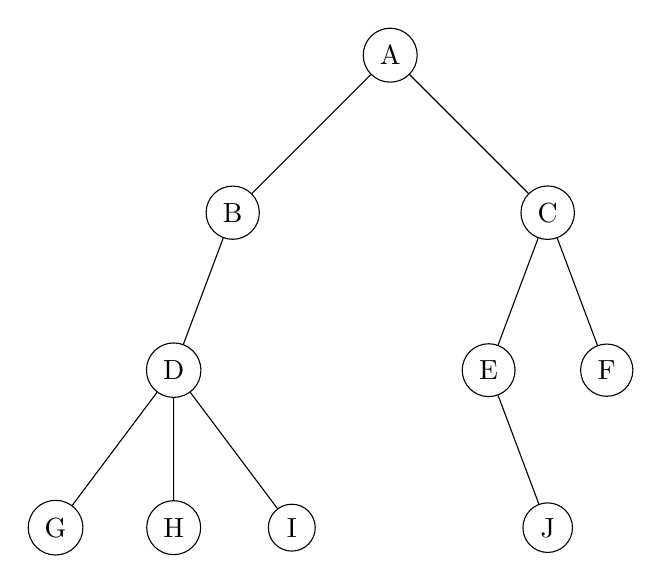
\begin{tikzpicture}[
			level distance=2cm,
			level 1/.style={sibling distance=4cm},
			level 2/.style={sibling distance=1.5cm},
			level 3/.style={sibling distance=1.5cm}
		]
		\node[circle,draw] {A}
		child {
				node[circle,draw] {B}
				child {
						node[circle,draw] {D}
						child {node[circle,draw] {G}}
						child {node[circle,draw] {H}}
						child {node[circle,draw] {I}}
					}
				child[missing] {}
			}
		child {
				node[circle,draw] {C}
				child {
						node[circle,draw] {E}
						child[missing] {}
						child {node[circle,draw] {J}}
					}
				child {node[circle,draw] {F}}
			};
	\end{tikzpicture}
	\caption{树}
\end{figure}

\begin{itemize}
	\item 根:没有父结点(parent)的结点。

	\item 内部结点(internal node):至少有一个子结点(child)的结点。

	\item 外部结点(external node) / 叶子结点(leaf node):没有子结点的结点。

	\item 度(degree):结点分支的个数。

	\item 路径(path):从根结点到树中某结点经过的分支构成了路径。

	\item 祖先结点(ancestors):包含父结点、父结点的父结点等。

	\item 子孙结点(descendants):包含子结点、子结点的子结点等。

	\item 深度(depth) / 高度(height):最大层级数。
\end{itemize}

\newpage

\section{二叉树}

\subsection{二叉树(Binary Tree)}

二叉树是树的一种特殊形式。二叉树的每个结点最多有两个孩子结点,即最多有2个,也可能只有1个,或者没有孩子结点。\\

二叉树结点的两个孩子结点,分别被称为左孩子(left child)和右孩子(right child)。这两个孩子结点的顺序是固定的,不能颠倒或混淆。\\

\begin{figure}[H]
	\centering
	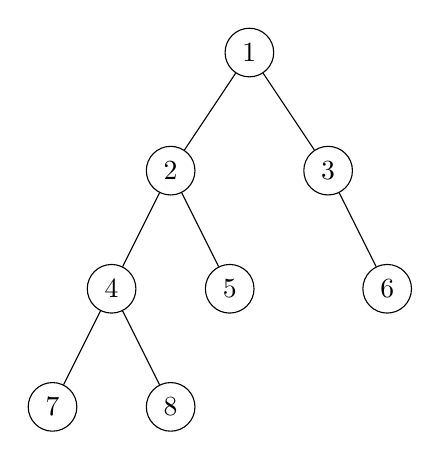
\begin{tikzpicture}[
			level distance=1.5cm,
			level 1/.style={sibling distance=2cm},
			level 2/.style={sibling distance=1.5cm},
			level 3/.style={sibling distance=1.5cm}
		]
		\node[circle,draw] {1}
		child {
				node[circle,draw] {2}
				child {
						node[circle,draw] {4}
						child {node[circle,draw] {7}}
						child {node[circle,draw] {8}}
					}
				child {node[circle,draw] {5}}
			}
		child {
				node[circle,draw] {3}
				child[missing] {}
				child {node[circle,draw] {6}}
			};
	\end{tikzpicture}
	\caption{二叉树}
\end{figure}

二叉树还有几种特殊的形式:

\subsubsection{左斜树(left skew tree) / 右斜树(right skew tree)}

只有左子树或只有右子树的二叉树。\\

\begin{figure}[H]
	\centering
	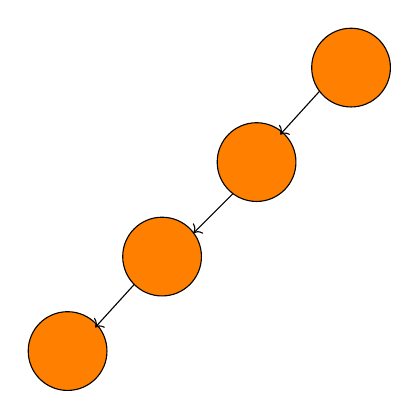
\begin{tikzpicture}
		\draw[fill=orange] (0,0) circle (0.5);
		\draw[fill=orange] (-1.2,-1.2) circle (0.5);
		\draw[fill=orange] (-2.4,-2.4) circle (0.5);
		\draw[fill=orange] (-3.6,-3.6) circle (0.5);

		\draw[->] (-0.4,-0.3) -- (-0.9,-0.85);
		\draw[->] (-1.5,-1.6) -- (-2,-2.1);
		\draw[->] (-2.75,-2.75) -- (-3.25,-3.3);
	\end{tikzpicture}
	\caption{左斜树}
\end{figure}

\subsubsection{满二叉树(full binary tree)}

所有非叶子结点都存在左右孩子,并且所有叶子结点都在同一层。\\

\begin{figure}[H]
	\centering
	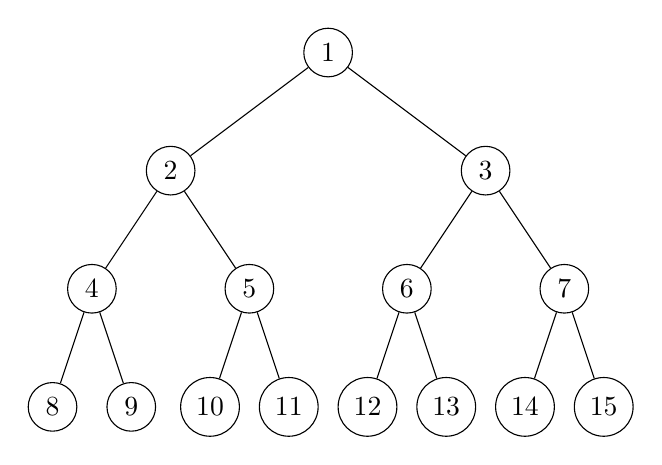
\begin{tikzpicture}[
			level distance=1.5cm,
			level 1/.style={sibling distance=4cm},
			level 2/.style={sibling distance=2cm},
			level 3/.style={sibling distance=1cm}
		]
		\node[circle,draw] {1}
		child {
				node[circle,draw] {2}
				child {
						node[circle,draw] {4}
						child {node[circle,draw] {8}}
						child {node[circle,draw] {9}}
					}
				child {
						node[circle,draw] {5}
						child {node[circle,draw] {10}}
						child {node[circle,draw] {11}}
					}
			}
		child {
				node[circle,draw] {3}
				child {
						node[circle,draw] {6}
						child {node[circle,draw] {12}}
						child {node[circle,draw] {13}}
					}
				child {
						node[circle,draw] {7}
						child {node[circle,draw] {14}}
						child {node[circle,draw] {15}}
					}
			};
	\end{tikzpicture}
	\caption{满二叉树}
\end{figure}

\subsubsection{完全二叉树}

对于一个有n个结点的二叉树,按层级顺序编号,则所有结点的编号从1到n,完全二叉树所有结点和同样深度的满二叉树的编号从1到n的结点位置相同。简单来说,就是除最后一层外,其它各层的结点数都达到最大,并且最后一层从右向左连续缺少若干个结点。\\

\begin{figure}[H]
	\centering
	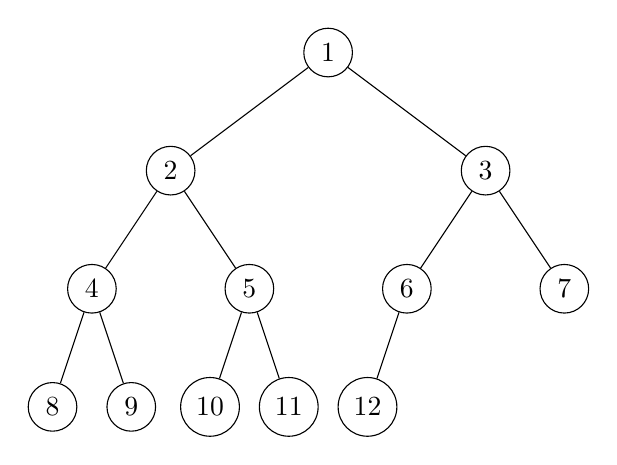
\begin{tikzpicture}[
			level distance=1.5cm,
			level 1/.style={sibling distance=4cm},
			level 2/.style={sibling distance=2cm},
			level 3/.style={sibling distance=1cm}
		]
		\node[circle,draw] {1}
		child {
				node[circle,draw] {2}
				child {
						node[circle,draw] {4}
						child {node[circle,draw] {8}}
						child {node[circle,draw] {9}}
					}
				child {
						node[circle,draw] {5}
						child {node[circle,draw] {10}}
						child {node[circle,draw] {11}}
					}
			}
		child {
				node[circle,draw] {3}
				child {
						node[circle,draw] {6}
						child {node[circle,draw] {12}}
						child[missing] {}
					}
				child {node[circle,draw] {7}}
			};
	\end{tikzpicture}
	\caption{完全二叉树}
\end{figure}

\newpage

\section{二叉树的遍历}

\subsection{二叉树的遍历}

在计算机程序中,遍历(traversal)本身是一个线性操作,所以遍历同样具有线性结构的数组或链表是一件轻而易举的事情。\\

反观二叉树,是典型的非线性数据结构,遍历时需要把非线性关联的结点转化成一个线性的序列,以不同的方式来遍历,遍历出的序列顺序也不同。\\

二叉树的遍历方式分为4种:

\begin{enumerate}
	\item 前序遍历(pre-order):访问根结点,遍历左子树,遍历右子树。

	\item 中序遍历(in-order):遍历左子树,访问根结点,遍历右子树。

	\item 后序遍历(post-order):遍历左子树,遍历右子树,访问根结点。

	\item 层次遍历(level-order):按照从根结点到叶子结点的层次关系,一层一层横向遍历。
\end{enumerate}

\vspace{0.5cm}

\subsection{前序遍历}

二叉树的前序遍历,首先访问根结点然后遍历左子树,最后遍历右子树。在遍历左、右子树时,仍然先访问根结点,然后遍历左子树,最后遍历右子树,如果结点为空则返回。\\

\begin{figure}[H]
	\centering
	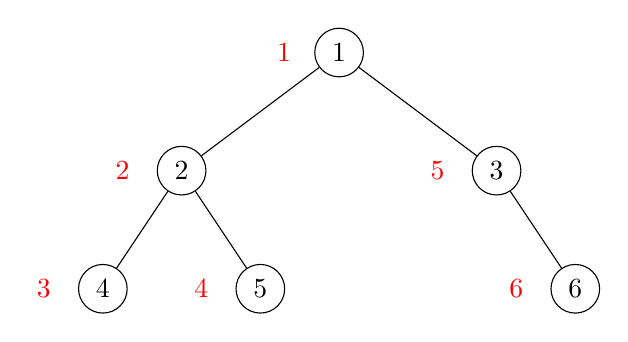
\begin{tikzpicture}[
			level distance=1.5cm,
			level 1/.style={sibling distance=4cm},
			level 2/.style={sibling distance=2cm},
			level 3/.style={sibling distance=1cm}
		]
		\node[circle,draw] {1}
		child {
				node[circle,draw] {2}
				child {
						node[circle,draw] {4}
					}
				child {
						node[circle,draw] {5}
					}
			}
		child {
				node[circle,draw] {3}
				child[missing] {}
				child {node[circle,draw] {6}}
			};

		\draw[color=red] (-0.7,0) node{1};
		\draw[color=red] (-2.75,-1.5) node{2};
		\draw[color=red] (-3.75,-3) node{3};
		\draw[color=red] (-1.75,-3) node{4};
		\draw[color=red] (1.25,-1.5) node{5};
		\draw[color=red] (2.25,-3) node{6};
	\end{tikzpicture}
	\caption{前序遍历}
\end{figure}

\vspace{0.5cm}

\subsection{中序遍历}

二叉树的中序遍历,首先遍历左子树,然后访问根结点,最后遍历右子树,如果结点为空则返回。\\

\begin{figure}[H]
	\centering
	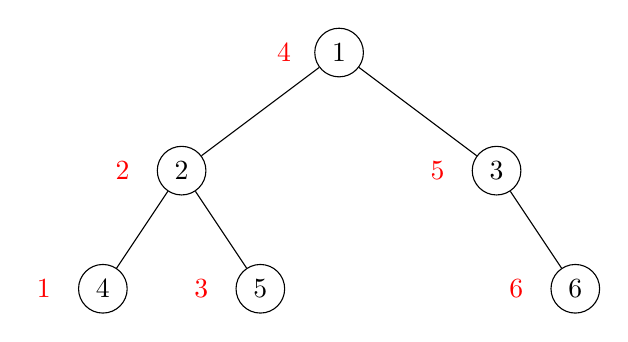
\begin{tikzpicture}[
			level distance=1.5cm,
			level 1/.style={sibling distance=4cm},
			level 2/.style={sibling distance=2cm},
			level 3/.style={sibling distance=1cm}
		]
		\node[circle,draw] {1}
		child {
				node[circle,draw] {2}
				child {
						node[circle,draw] {4}
					}
				child {
						node[circle,draw] {5}
					}
			}
		child {
				node[circle,draw] {3}
				child[missing] {}
				child {node[circle,draw] {6}}
			};

		\draw[color=red] (-0.7,0) node{4};
		\draw[color=red] (-2.75,-1.5) node{2};
		\draw[color=red] (-3.75,-3) node{1};
		\draw[color=red] (-1.75,-3) node{3};
		\draw[color=red] (1.25,-1.5) node{5};
		\draw[color=red] (2.25,-3) node{6};
	\end{tikzpicture}
	\caption{中序遍历}
\end{figure}

\vspace{0.5cm}

\subsection{后序遍历}

二叉树的后序遍历,首先遍历左子树,然后遍历右子树,最后访问根结点,如果结点为空则返回。\\

\begin{figure}[H]
	\centering
	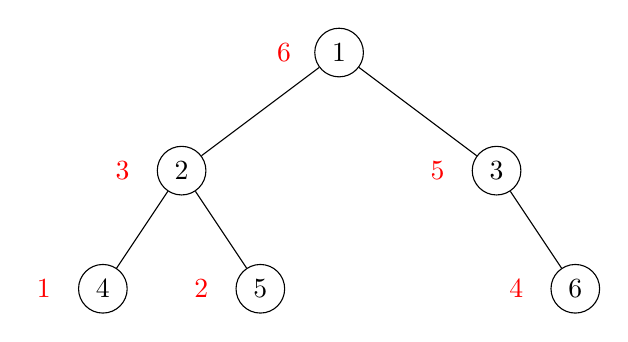
\begin{tikzpicture}[
			level distance=1.5cm,
			level 1/.style={sibling distance=4cm},
			level 2/.style={sibling distance=2cm},
			level 3/.style={sibling distance=1cm}
		]
		\node[circle,draw] {1}
		child {
				node[circle,draw] {2}
				child {
						node[circle,draw] {4}
					}
				child {
						node[circle,draw] {5}
					}
			}
		child {
				node[circle,draw] {3}
				child[missing] {}
				child {node[circle,draw] {6}}
			};

		\draw[color=red] (-0.7,0) node{6};
		\draw[color=red] (-2.75,-1.5) node{3};
		\draw[color=red] (-3.75,-3) node{1};
		\draw[color=red] (-1.75,-3) node{2};
		\draw[color=red] (1.25,-1.5) node{5};
		\draw[color=red] (2.25,-3) node{4};
	\end{tikzpicture}
	\caption{后序遍历}
\end{figure}

\newpage

\section{二叉搜索树}

\subsection{二叉搜索树(Binary Search Tree)}

二叉搜索树,也称二叉查找树或二叉排序树,可以是一棵空树。\\

如果不为空树,那么二叉搜索树满足以下性质:

\begin{enumerate}
	\item 非空左子树的所有结点的值小于其根结点的值。
	\item 非空右子树的所有结点的值大于其根结点的值。
	\item 左、右子树均是二叉搜索树。
\end{enumerate}

\begin{figure}[H]
	\centering
	\begin{tikzpicture}[
			level distance=1.5cm,
			level 1/.style={sibling distance=4cm},
			level 2/.style={sibling distance=2cm},
			level 3/.style={sibling distance=1cm}
		]
		\node[circle,draw] {6}
		child {
				node[circle,draw] {3}
				child {
						node[circle,draw] {2}
						child {node[circle,draw] {1}}
						child[missing] {}
					}
				child {node[circle,draw] {4}}
			}
		child {
				node[circle,draw] {8}
				child {node[circle,draw] {7}}
				child {node[circle,draw] {9}}
			};
	\end{tikzpicture}
	\caption{二叉搜索树}
\end{figure}

\vspace{0.5cm}

\subsection{查找结点}

在二叉搜索树中查找一个元素从根结点开始,如果树为空,返回NULL。\\

如果树不为空,则将根结点的值和被查找的key值进行比较:

\begin{enumerate}
	\item 如果key值小于根结点的值,只需在左子树中继续查找。
	\item 如果key值大于根结点的值,只需在右子树中继续查找。
	\item 如果key值与根结点的值相等,查找成功。
\end{enumerate}

二叉搜索树中,最小值一定在树的最左分枝的叶子结点上,最大值一定在树的最右分枝的叶子结点上。

\newpage

\section{哈夫曼树}

\subsection{哈夫曼树(Huffman Tree)}

树的每一个结点都可以拥有自己的权值(weight),假设二叉树有n个叶子结点,每个叶子结点都带有权值$ w_k $,从根结点到每个叶子结点的长度为$ l_k $,则树的带权路径长度(WPL, Weighted Path Length)为:

$$
	WPL = \sum_{k=1}^n w_k l_k
$$

哈夫曼树是由麻省理工学院的哈夫曼博士于1952年发明的,哈夫曼树是在叶子结点和权重确定的情况下,带权路径长度最小的二叉树,也被称为最优二叉树。\\

例如,有五个叶子结点,它们的权值为\{1, 2, 3, 4, 5\},用此权值序列可以构造出形状不同的多个二叉树。\\

\begin{figure}[H]
	\centering
	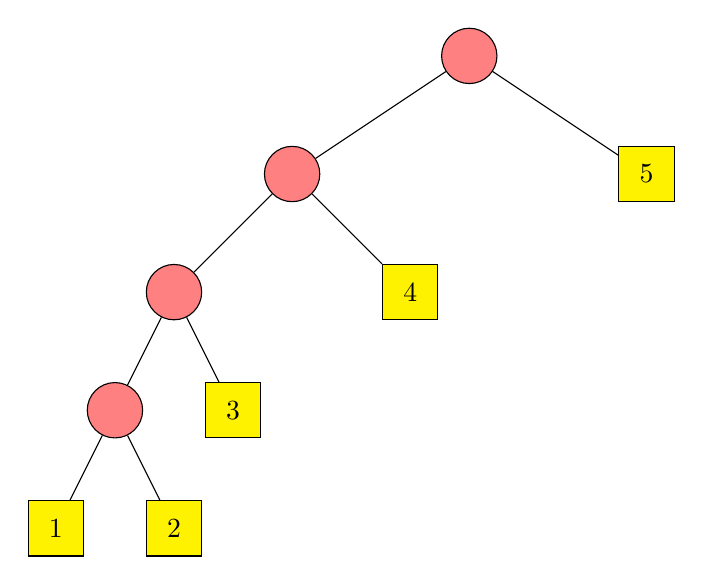
\begin{tikzpicture}[iv/.style={draw,fill=red!50,circle,minimum size=20pt,inner
					sep=0pt,text=black},ev/.style={draw,fill=yellow,rectangle,minimum
					size=20pt,inner sep=0pt,text=black}]
		\node[iv]{}
		child {node[iv]{}
				child {node[iv]{}
						child {node[iv]{}
								child {node[ev]{1}}
								child {node[ev]{2}}
							}
						child {node[ev]{3}}
					}
				child [missing]
				child {node[ev]{4}}
			}
		child [missing]
		child [missing]
		child {node[ev]{5}};
	\end{tikzpicture}
	\caption{WPL = 5 * 1 + 4 * 2 + 3 * 3 + 2 * 4 + 1 * 4 = 34}
\end{figure}

\begin{figure}[H]
	\centering
	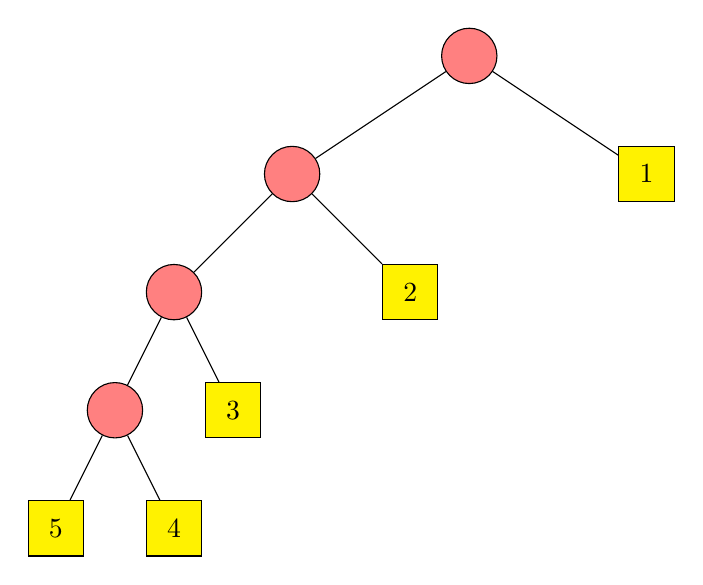
\begin{tikzpicture}[iv/.style={draw,fill=red!50,circle,minimum size=20pt,inner
					sep=0pt,text=black},ev/.style={draw,fill=yellow,rectangle,minimum
					size=20pt,inner sep=0pt,text=black}]
		\node[iv]{}
		child {node[iv]{}
				child {node[iv]{}
						child {node[iv]{}
								child {node[ev]{5}}
								child {node[ev]{4}}
							}
						child {node[ev]{3}}
					}
				child [missing]
				child {node[ev]{2}}
			}
		child [missing]
		child [missing]
		child {node[ev]{1}};
	\end{tikzpicture}
	\caption{WPL = 1 * 1 + 2 * 2 + 3 * 3 + 4 * 4 + 5 * 4 = 50}
\end{figure}

\begin{figure}[H]
	\centering
	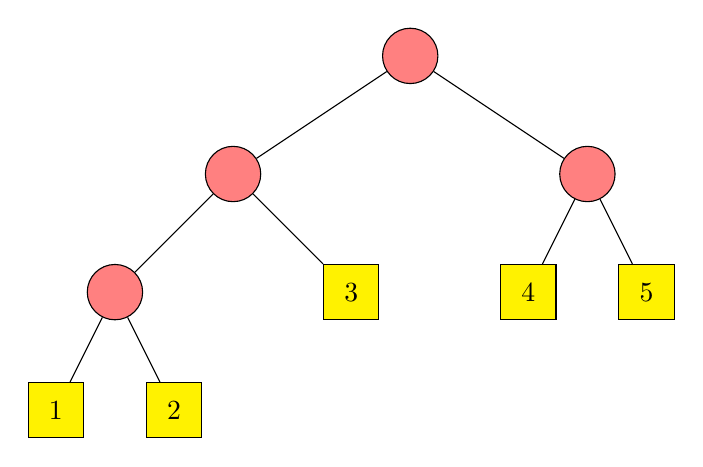
\begin{tikzpicture}[iv/.style={draw,fill=red!50,circle,minimum size=20pt,inner
					sep=0pt,text=black},ev/.style={draw,fill=yellow,rectangle,minimum
					size=20pt,inner sep=0pt,text=black}]
		\node[iv]{}
		child {node[iv]{}
				child {node[iv]{}
						child {node[ev]{1}}
						child {node[ev]{2}}
					}
				child [missing]
				child {node[ev]{3}}
			}
		child [missing]
		child [missing]
		child {node[iv]{}
				child {node[ev]{4}}
				child {node[ev]{5}}
			};
	\end{tikzpicture}
	\caption{WPL = 3 * 2 + 4 * 2 + 5 * 2 + 1 * 3 + 2 * 3 = 33}
\end{figure}

怎样才能保证构建出的二叉树带权路径长度最小呢?原则上,应该让权重小的叶子结点远离树根,权重大的叶子结点靠近树根。需要注意的是,同样叶子结点所构成的哈夫曼树可能不止一棵。\\

\subsection{哈夫曼树的构造}

哈夫曼树的构造方法就是每次把权值最小的两棵二叉树合并。\\

例如有6个叶子结点,权重依次是2、3、7、9、18、25。\\

第一步:把每一个叶子结点都当成一棵独立的树(只有根结点的树),这样就形成了一个森林。

\begin{figure}[H]
	\centering
	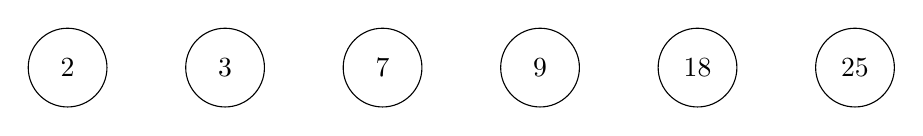
\begin{tikzpicture}
		\draw (0,0) circle (0.5) node{2};
		\draw (2,0) circle (0.5) node{3};
		\draw (4,0) circle (0.5) node{7};
		\draw (6,0) circle (0.5) node{9};
		\draw (8,0) circle (0.5) node{18};
		\draw (10,0) circle (0.5) node{25};
	\end{tikzpicture}
\end{figure}

第二步:从森林中移除权值最小的两个结点,生成父结点,父结点的权值是这两个结点权值之和,把父结点加入森林。重复该步骤,直到森林中只有一棵树为止。\\

\begin{figure}[H]
	\centering
	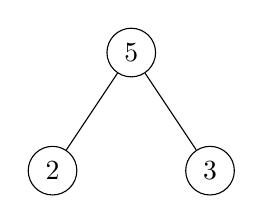
\begin{tikzpicture}[
			level distance=1.5cm,
			level 1/.style={sibling distance=2cm},
			level 2/.style={sibling distance=1.5cm},
			level 3/.style={sibling distance=1.5cm}
		]
		\node[circle,draw] {5}
		child {node[circle,draw] {2}}
		child {node[circle,draw] {3}};
	\end{tikzpicture}
	\caption{合并2和3}
\end{figure}

\begin{figure}[H]
	\centering
	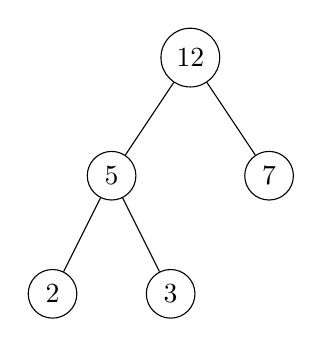
\begin{tikzpicture}[
			level distance=1.5cm,
			level 1/.style={sibling distance=2cm},
			level 2/.style={sibling distance=1.5cm},
			level 3/.style={sibling distance=1.5cm}
		]
		\node[circle,draw] {12}
		child {
				node[circle,draw] {5}
				child {node[circle,draw] {2}}
				child {node[circle,draw] {3}}
			}
		child {node[circle,draw] {7}};
	\end{tikzpicture}
	\caption{合并5和7}
\end{figure}

\begin{figure}[H]
	\centering
	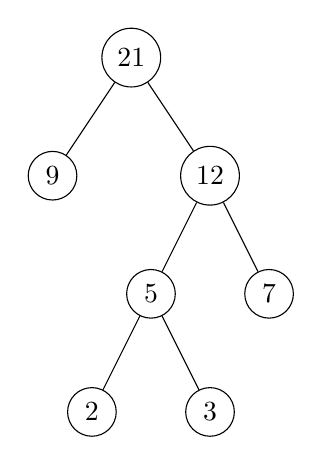
\begin{tikzpicture}[
			level distance=1.5cm,
			level 1/.style={sibling distance=2cm},
			level 2/.style={sibling distance=1.5cm},
			level 3/.style={sibling distance=1.5cm}
		]
		\node[circle,draw] {21}
		child {node[circle,draw] {9}}
		child {
				node[circle,draw] {12}
				child {
						node[circle,draw] {5}
						child {node[circle,draw] {2}}
						child {node[circle,draw] {3}}
					}
				child {node[circle,draw] {7}}
			};
	\end{tikzpicture}
	\caption{合并9和12}
\end{figure}

\begin{figure}[H]
	\centering
	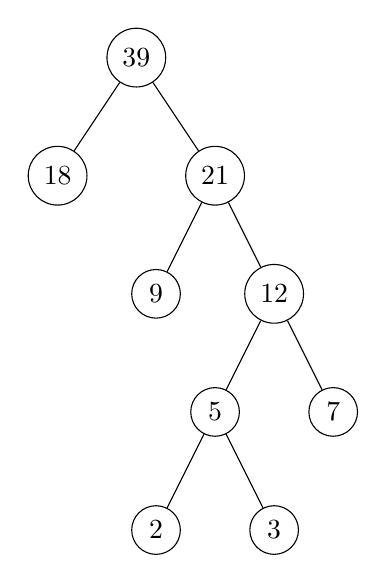
\begin{tikzpicture}[
			level distance=1.5cm,
			level 1/.style={sibling distance=2cm},
			level 2/.style={sibling distance=1.5cm},
			level 3/.style={sibling distance=1.5cm}
		]
		\node[circle,draw] {39}
		child {node[circle,draw] {18}}
		child {
				node[circle,draw] {21}
				child {node[circle,draw] {9}}
				child {
						node[circle,draw] {12}
						child {
								node[circle,draw] {5}
								child {node[circle,draw] {2}}
								child {node[circle,draw] {3}}
							}
						child {node[circle,draw] {7}}
					}
			};
	\end{tikzpicture}
	\caption{合并18和21}
\end{figure}

\begin{figure}[H]
	\centering
	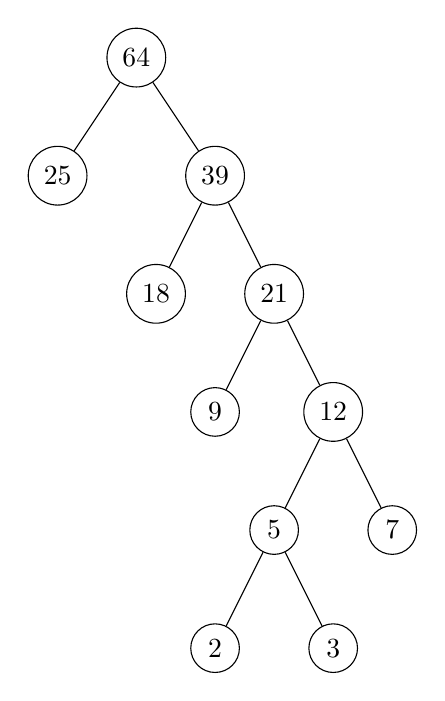
\begin{tikzpicture}[
			level distance=1.5cm,
			level 1/.style={sibling distance=2cm},
			level 2/.style={sibling distance=1.5cm},
			level 3/.style={sibling distance=1.5cm}
		]
		\node[circle,draw] {64}
		child {node[circle,draw] {25}}
		child {
				node[circle,draw] {39}
				child {node[circle,draw] {18}}
				child {
						node[circle,draw] {21}
						child {node[circle,draw] {9}}
						child {
								node[circle,draw] {12}
								child {
										node[circle,draw] {5}
										child {node[circle,draw] {2}}
										child {node[circle,draw] {3}}
									}
								child {node[circle,draw] {7}}
							}
					}
			};
	\end{tikzpicture}
	\caption{合并25和39}
\end{figure}

哈夫曼树有以下几个特点:

\begin{enumerate}
	\item 没有度为1的结点。
	\item 哈夫曼树的任意非叶结点的左右子树交换后仍是哈夫曼树。
	\item 对同一组权值,可能存在不同构的两棵哈夫曼树。
\end{enumerate}

\begin{figure}[H]
	\centering
	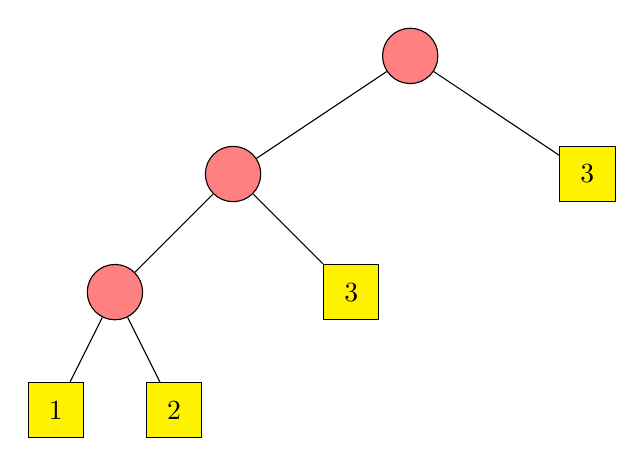
\begin{tikzpicture}[iv/.style={draw,fill=red!50,circle,minimum size=20pt,inner
					sep=0pt,text=black},ev/.style={draw,fill=yellow,rectangle,minimum
					size=20pt,inner sep=0pt,text=black}]
		\node[iv]{}
		child {node[iv]{}
				child {node[iv]{}
						child {node[ev]{1} }
						child {node[ev]{2}}
					}
				child [missing]
				child {node[ev]{3}}
			}
		child [missing]
		child [missing]
		child {node[ev]{3}};
	\end{tikzpicture}
	\caption{WPL = 3 * 1 + 3 * 2 + 1 * 3 + 2 * 3 = 18}
\end{figure}

\begin{figure}[H]
	\centering
	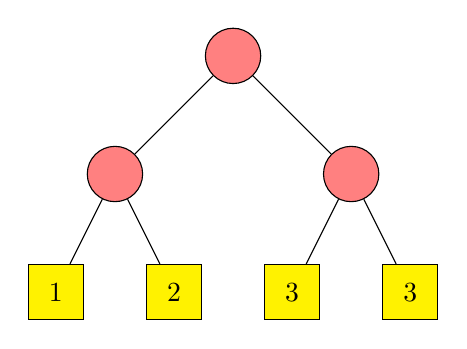
\begin{tikzpicture}[iv/.style={draw,fill=red!50,circle,minimum size=20pt,inner
					sep=0pt,text=black},ev/.style={draw,fill=yellow,rectangle,minimum
					size=20pt,inner sep=0pt,text=black}]
		\node[iv]{}
		child {node[iv]{}
				child {node[ev]{1}}
				child {node[ev]{2}}
			}
		child [missing]
		child {
				node[iv]{}
				child {node[ev]{3}}
				child {node[ev]{3}}
			};
	\end{tikzpicture}
	\caption{WPL = 1 * 2 + 2 * 2 + 3 * 2 + 3 * 2 = 18}
\end{figure}

\newpage

\section{哈夫曼编码}

\subsection{哈夫曼编码(Huffman Code)}

哈夫曼编码是一种高效的编码方式,在信息存储和传输过程中用于对信息进行压缩。要理解哈夫曼编码,需要从信息存储的底层逻辑讲起。\\

计算机不是人,它不认识中文和英文,更不认识图片和视频,它唯一认识的就是0(低电平)和1(高电平)。因此,计算机上一切文字、图象、音频、视频,底层都是用二进制来存储和传输的。\\

将信息转换成计算机能够识别的二进制形式的过程被称为编码。在ASCII码中,每一个字符表示成特定的8位二进制数。例如字符串APPLE表示成8位二进制编码为01000001 01010000 01010000 01001100 01000101。\\

显然,ASCII码是一种等长编码,也就是任何字符的编码长度都相等。等长编码的有点明显,因为每个字符对应的二进制编码长度相等,所以很容易设计,也很方便读写。但是计算机的存储空间以及网络传输的带宽是有限的,等长编码最大的缺点就是编码结果太长,会占用过多资源。\\

使用不等长编码,让出现频率高的字符用的编码短一些,出现频率低的字符编码长一些,可以使编码的总长度减小。但是不等长编码是不能随意设计的,如果一个字符的编码恰好是另一个字符编码的前缀,就会产生歧义的问题。\\

哈夫曼编码就是一种不等长的编码,并且任何一个字符的编码都不是另一个字符编码的前缀,因此可以无二义地进行解码,并且信息编码的总长度最小。\\

哈夫曼编码并非一套固定的编码,而是根据给定信息中各个字符出现的频次,动态生成最优的编码。哈夫曼编码的生成过程就用到了哈夫曼树。\\

例如一段信息里只有A、B、C、D、E、F这6个字符,出现的次数分别是2次、3次、7次、9次、18次、25次。通过把这6个字符当成6个叶子结点,将出现次数作为结点的权重,生成一颗哈夫曼树。将哈夫曼树中结点的左分支当做0、结点的右分支当做1,从哈夫曼树的根结点到每一个叶子结点的路径,都可以等价为一段二进制编码。\\

\begin{figure}[H]
	\centering
	\begin{forest}
		for tree={where n children={0}{ev}{iv},l+=8mm,
		if n=1{edge label={node [midway, left] {0} } }{edge label={node [midway, right] {1} } },}
		[
		[F]
			[
				[E]
					[
						[D]
							[
								[
										[A]
											[B]
									]
									[C]
							]
					]
			]
		]
	\end{forest}
\end{figure}

\begin{table}[H]
	\centering
	\setlength{\tabcolsep}{5mm}{
		\begin{tabular}{|c|c|}
			\hline
			\textbf{字符} & \textbf{编码} \\
			\hline
			\textbf{A}    & 11100         \\
			\hline
			\textbf{B}    & 11101         \\
			\hline
			\textbf{C}    & 1111          \\
			\hline
			\textbf{D}    & 110           \\
			\hline
			\textbf{E}    & 10            \\
			\hline
			\textbf{F}    & 0             \\
			\hline
		\end{tabular}
	}
	\caption{哈夫曼编码}
\end{table}

因为每一个字符对应的都是哈夫曼树的叶子结点,从根结点到这些叶子结点的路径并没有包含关系,最终得到的二进制编码自然也不会是彼此的前缀。

\newpage
\chapter{图}

\section{图}

\subsection{图(Graph)}

你的微信中有若干好友,而你的好友又有若干好友。许许多多的用户组成了一个多对多的关系网,这个关系网就是数据结构中的图。\\

再例如使用地图导航功能时,导航会根据你的出发地和目的地规划最佳的地铁换乘路线。许许多多的地铁站组成的交通网络也可以认为是图。\\

图是一种比树更为复杂的数据结构。树的结点之间是一对多的关系,并且存在父与子的层级划分。而图的顶点之间是多对多关系,并且所有顶点都是平等的,无所谓谁是父子。\\

在图中,最基本的单元是顶点(vertex),相当于树中的结点。顶点之间的关联关系被称为边(edge)。图中包含一组顶点和一组边,通常用V表示顶点集合,用E表示边集合。边可以看作是顶点对,即$ (v, w) \in E,\ v, w \in V $。\\

在有些图中,每一条边并不是完全等同的。例如地铁线路,站与站之间的距离都有可能不同。因此图中会涉及边的权重(weight),涉及到权重的图被称为带权图(weighted graph),也称为网络。

\begin{figure}[H]
	\centering
	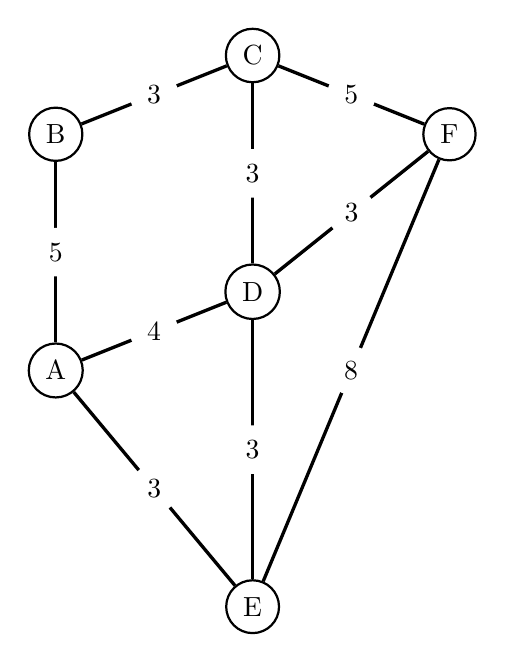
\begin{tikzpicture}
		\begin{scope}[every node/.style={circle,thick,draw}]
			\node (A) at (0,0) {A};
			\node (B) at (0,3) {B};
			\node (C) at (2.5,4) {C};
			\node (D) at (2.5,1) {D};
			\node (E) at (2.5,-3) {E};
			\node (F) at (5,3) {F};
		\end{scope}

		\begin{scope}[>={Stealth[black]},
			every node/.style={fill=white,circle},
			every edge/.style={draw=black,very thick}]
			\path [-] (A) edge node {5} (B);
			\path [-] (B) edge node {3} (C);
			\path [-] (A) edge node {4} (D);
			\path [-] (D) edge node {3} (C);
			\path [-] (A) edge node {3} (E);
			\path [-] (D) edge node {3} (E);
			\path [-] (D) edge node {3} (F);
			\path [-] (C) edge node {5} (F);
			\path [-] (E) edge node {8} (F);
		\end{scope}
	\end{tikzpicture}
	\caption{带权图}
\end{figure}

还有一种图,顶点之间的关联并不是完全对称的。拿微信举例,你的好友列表里有我,但我的好友列表里未必有你。\\

这样一来,顶点之间的边就有了方向的区分,这种带有方向的图被称为有向图(directed graph)。有向边可以使用<v, w>表示从v指向w的边。\\

\begin{figure}[H]
	\centering
	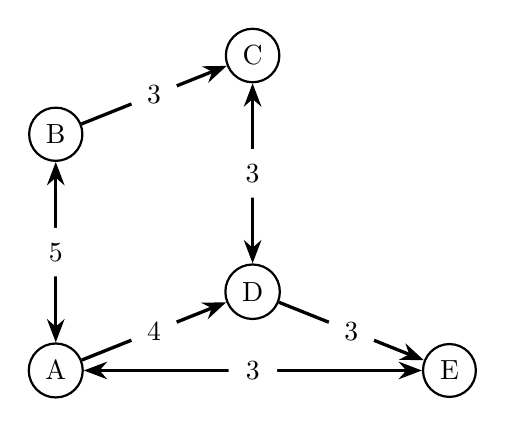
\begin{tikzpicture}
		\begin{scope}[every node/.style={circle,thick,draw}]
			\node (A) at (0,0) {A};
			\node (B) at (0,3) {B};
			\node (C) at (2.5,4) {C};
			\node (D) at (2.5,1) {D};
			\node (E) at (5,0) {E};
		\end{scope}

		\begin{scope}[>={Stealth[black]},
			every node/.style={fill=white,circle},
			every edge/.style={draw=black,very thick}]
			\path [<->] (A) edge node {5} (B);
			\path [->] (B) edge node {3} (C);
			\path [->] (A) edge node {4} (D);
			\path [<->] (D) edge node {3} (C);
			\path [<->] (A) edge node {3} (E);
			\path [->] (D) edge node {3} (E);
		\end{scope}
	\end{tikzpicture}
	\caption{有向图}
\end{figure}

相应地,在QQ中,只要我把你从好友里删除,你在自己的好友列表里就看不到我了。因此QQ的好友关系可以认为是一个没有方向区分的图,这种图被称为无向图(undirected graph)。

\vspace{0.5cm}

\subsection{图的术语}

图还有一些有关路径的术语:

\begin{itemize}
	\item 度:一个顶点的度是指与该顶点相关联的边的条数。

	\item 入度:对于有向图,入度为以该顶点为终点的边数。

	\item 出度:对于有向图,入度为以该顶点为起点的边数。

	\item 连通:如果从顶点V到W存在一条路径,则称V和W是连通的。

	\item 路径:顶点V到W的路径是一系列顶点$ \{V, v_1, v_2, \dots, v_n, W\} $的集合,其中任意一对相邻的顶点间都有图中的边。

	\item 路径长度:路径中边的个数,如果是带权图(网络),则是所有边的权重和。

	\item 简单路径:顶点V到W之间的路径中所有顶点都不同。

	\item 回路:起点等于终点的路径。
\end{itemize}

\begin{tcolorbox}
	\mybox{握手定理Handshaking Theorem}\\
	假设$ G = (V, E) $是无向图,每条边都会给顶点的度之和增加2,则
	\begin{align}
		\sum_{v \in V} deg(v) = 2|E|
	\end{align}
\end{tcolorbox}

\begin{tcolorbox}
	\mybox{Exercise}
	一个有10个顶点,且每个顶点的度都为6的图,有多少条边?
	\begin{align*}
		2m & = 6 \times 10 \\
		m  & = 30
	\end{align*}
\end{tcolorbox}

\newpage

\section{图的表示}

\subsection{邻接矩阵(Adjacency Matrix)}

拥有n个顶点的图,它所包含的边的数量最多是n(n-1)条,因此,要表达各个顶点之间的关联关系,最清晰易懂的方式是使用邻接矩阵G[N][N]。\\

对于无向图来说,如果顶点之间有关联,那么邻接矩阵中对应的值为1;如果顶点之间没有关联,那么邻接矩阵中对应的值为0。

\vspace{-0.5cm}

\begin{align}\nonumber
	G[i][j] = \begin{cases}
		1 & <v_i, v_j>\text{是G中的边}   \\
		0 & <v_i, v_j>\text{不是G中的边} \\
	\end{cases}
\end{align}

\begin{figure}[H]
	\centering
	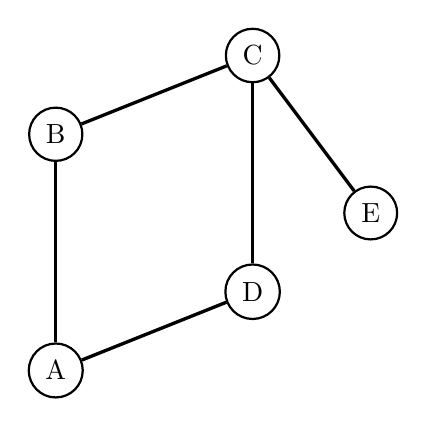
\begin{tikzpicture}
		\begin{scope}[every node/.style={circle,thick,draw}]
			\node (A) at (0,0) {A};
			\node (B) at (0,3) {B};
			\node (C) at (2.5,4) {C};
			\node (D) at (2.5,1) {D};
			\node (E) at (4,2) {E};
		\end{scope}

		\begin{scope}[>={Stealth[black]},
			every node/.style={},
			every edge/.style={draw=black,very thick}]
			\path [-] (A) edge node {} (B);
			\path [-] (A) edge node {} (D);
			\path [-] (B) edge node {} (C);
			\path [-] (C) edge node {} (D);
			\path [-] (C) edge node {} (E);
		\end{scope}
	\end{tikzpicture}
\end{figure}

\begin{table}[H]
	\centering
	\setlength{\tabcolsep}{5mm}{
		\begin{tabular}{|c|c|c|c|c|c|}
			\hline
			           & \textbf{A} & \textbf{B} & \textbf{C} & \textbf{D} & \textbf{E} \\
			\hline
			\textbf{A} & 0          & 1          & 0          & 1          & 0          \\
			\hline
			\textbf{B} & 1          & 0          & 1          & 0          & 0          \\
			\hline
			\textbf{C} & 0          & 1          & 0          & 1          & 1          \\
			\hline
			\textbf{D} & 1          & 0          & 1          & 0          & 0          \\
			\hline
			\textbf{E} & 0          & 0          & 1          & 0          & 0          \\
			\hline
		\end{tabular}
	}
	\caption{无向图邻接矩阵}
\end{table}

需要注意的是,邻接矩阵从左上到右下的一条对角线上的元素值必然是0,因为任何一个顶点与它自身是没有连接的。同时,无向图对应的邻接矩阵是一个对称矩阵,假如A和B有关联,那么B和A也必定有关联。\\

但是对于有向图的邻接矩阵,不一定是一个对称矩阵,假如A可以达到B,从B未必能达到A。\\

\begin{figure}[H]
	\centering
	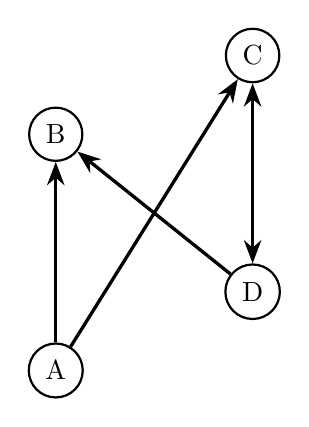
\begin{tikzpicture}
		\begin{scope}[every node/.style={circle,thick,draw}]
			\node (A) at (0,0) {A};
			\node (B) at (0,3) {B};
			\node (C) at (2.5,4) {C};
			\node (D) at (2.5,1) {D};
		\end{scope}

		\begin{scope}[>={Stealth[black]},
			every node/.style={},
			every edge/.style={draw=black,very thick}]
			\path [->] (A) edge node {} (B);
			\path [->] (A) edge node {} (C);
			\path [<->] (C) edge node {} (D);
			\path [->] (D) edge node {} (B);
		\end{scope}
	\end{tikzpicture}
\end{figure}

\begin{table}[H]
	\centering
	\setlength{\tabcolsep}{5mm}{
		\begin{tabular}{|c|c|c|c|c|}
			\hline
			           & \textbf{A} & \textbf{B} & \textbf{C} & \textbf{D} \\
			\hline
			\textbf{A} & 0          & 1          & 1          & 0          \\
			\hline
			\textbf{B} & 0          & 0          & 0          & 0          \\
			\hline
			\textbf{C} & 0          & 0          & 0          & 1          \\
			\hline
			\textbf{D} & 0          & 1          & 1          & 0          \\
			\hline
		\end{tabular}
	}
	\caption{有向图邻接矩阵}
\end{table}

对于网络,只要把邻接矩阵对应位置的值定义为边$ <v_i, v_j> $的权重即可。\\

\begin{figure}[H]
	\centering
	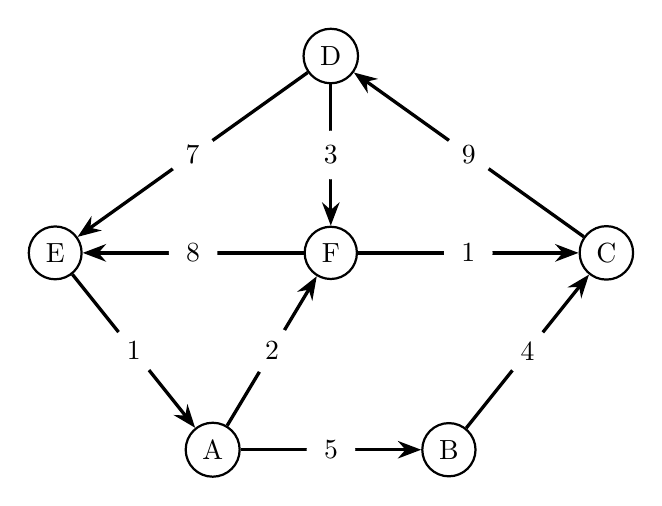
\begin{tikzpicture}
		\begin{scope}[every node/.style={circle,thick,draw}]
			\node (A) at (0,0) {A};
			\node (B) at (3,0) {B};
			\node (C) at (5,2.5) {C};
			\node (D) at (1.5,5) {D};
			\node (E) at (-2,2.5) {E};
			\node (F) at (1.5,2.5) {F};
		\end{scope}

		\begin{scope}[>={Stealth[black]},
			every node/.style={fill=white,circle},
			every edge/.style={draw=black,very thick}]
			\path [->] (A) edge node {5} (B);
			\path [->] (A) edge node {2} (F);
			\path [->] (B) edge node {4} (C);
			\path [->] (C) edge node {9} (D);
			\path [->] (D) edge node {7} (E);
			\path [->] (D) edge node {3} (F);
			\path [->] (E) edge node {1} (A);
			\path [->] (F) edge node {1} (C);
			\path [->] (F) edge node {8} (E);
		\end{scope}
	\end{tikzpicture}
\end{figure}

\begin{table}[H]
	\centering
	\setlength{\tabcolsep}{5mm}{
		\begin{tabular}{|c|c|c|c|c|c|c|}
			\hline
			           & \textbf{A} & \textbf{B} & \textbf{C} & \textbf{D} & \textbf{E} & \textbf{F} \\
			\hline
			\textbf{A} & $ \infty $ & 5          & $ \infty $ & $ \infty $ & $ \infty $ & 2          \\
			\hline
			\textbf{B} & $ \infty $ & $ \infty $ & 4          & $ \infty $ & $ \infty $ & $ \infty $ \\
			\hline
			\textbf{C} & $ \infty $ & $ \infty $ & $ \infty $ & 9          & $ \infty $ & $ \infty $ \\
			\hline
			\textbf{D} & $ \infty $ & $ \infty $ & $ \infty $ & $ \infty $ & 7          & 3          \\
			\hline
			\textbf{E} & 1          & $ \infty $ & $ \infty $ & $ \infty $ & $ \infty $ & $ \infty $ \\
			\hline
			\textbf{F} & $ \infty $ & $ \infty $ & 1          & $ \infty $ & 8          & $ \infty $ \\
			\hline
		\end{tabular}
	}
	\caption{带权图邻接矩阵}
\end{table}

对于带权图,如果$ v_i $和$ v_j $之前没有边应该将权值设为$ \infty $。\\

邻接矩阵的优点:

\begin{enumerate}
	\item 简单、直观。
	\item 可以快速查到一个顶点和另一顶点之间的关联关系。
	\item 方便计算任一顶点的度,对于有向图,从顶点发出的边数为出度,指向顶点的边数为入度。
\end{enumerate}

邻接矩阵的缺点:

\begin{enumerate}
	\item 浪费空间,对于稀疏图(点很多而边很少)有大量无效元素。但对于稠密图(特别是完全图)还是很合算的。
	\item 浪费时间,统计稀疏图中边的个数,也就是计算邻接矩阵中元素1的个数。
\end{enumerate}

\vspace{0.5cm}

\subsection{邻接表(Adjacency List)}

为了解决邻接矩阵占用空间的问题,人们想到了另一种图的表示方法——邻接表。在邻接表中,图的每一个顶点都是一个链表的头结点,其后连接着该顶点能够直接到达的相邻顶点。对于稀疏图而言,邻接表存储方式占用的空间比邻接矩阵要小得多。\\

\begin{figure}[H]
	\centering
	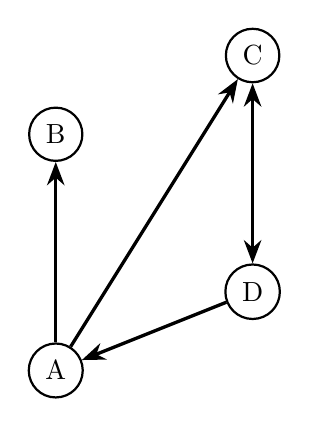
\begin{tikzpicture}
		\begin{scope}[every node/.style={circle,thick,draw}]
			\node (A) at (0,0) {A};
			\node (B) at (0,3) {B};
			\node (C) at (2.5,4) {C};
			\node (D) at (2.5,1) {D};
		\end{scope}

		\begin{scope}[>={Stealth[black]},
			every node/.style={},
			every edge/.style={draw=black,very thick}]
			\path [->] (A) edge node {} (B);
			\path [->] (A) edge node {} (C);
			\path [<->] (C) edge node {} (D);
			\path [->] (D) edge node {} (A);
		\end{scope}
	\end{tikzpicture}
\end{figure}

\begin{figure}[H]
	\centering
	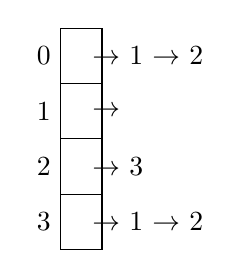
\begin{tikzpicture}
		\coordinate (0);
		\foreach \t[count=\i from 0,evaluate=\i as\j using int(\i+1)] in {
				1 $ \rightarrow $ 2,
				,
				3,
				1 $ \rightarrow $ 2
			}
		\node at(\i.south)[anchor=north,draw,minimum height=2em,minimum width=1.5em,outer sep=0pt](\j){}
		node at(\j.west)[align=right,left]{\i}
		node at(\j.east)[align=left,right,xshift=-.7em]{$ \rightarrow $ \t};
	\end{tikzpicture}
	\caption{邻接表}
\end{figure}

通过遍历邻接表可以查找到所有能够到达的相邻顶点,但是对于逆向查找,即哪些顶点可以达到一个顶点就会很麻烦。\\

逆邻接表和邻接表是正好相反的,逆邻接表每一个顶点作为链表的头结点,后继结点所存储的是能够直接到达该顶点的相邻顶点。

\begin{figure}[H]
	\centering
	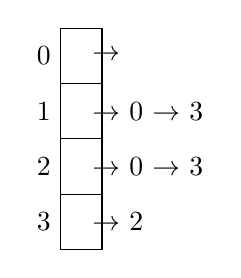
\begin{tikzpicture}
		\coordinate (0);
		\foreach \t[count=\i from 0,evaluate=\i as\j using int(\i+1)] in {
				,
				0 $ \rightarrow $ 3,
				0 $ \rightarrow $ 3,
				2
			}
		\node at(\i.south)[anchor=north,draw,minimum height=2em,minimum width=1.5em,outer sep=0pt](\j){}
		node at(\j.west)[align=right,left]{\i}
		node at(\j.east)[align=left,right,xshift=-.7em]{$ \rightarrow $ \t};
	\end{tikzpicture}
	\caption{逆邻接表}
\end{figure}

可是,一个图要维护正反两个邻接表,也太麻烦了吧?\\

通过十字链表可以把邻接表和逆邻接表结合在一起。\\

\begin{figure}[H]
	\centering
	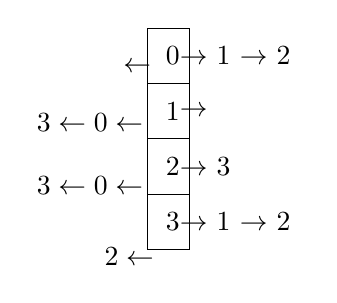
\begin{tikzpicture}
		\coordinate (0);
		\foreach \t[count=\i from 0,evaluate=\i as\j using int(\i+1)] in {
				1 $ \rightarrow $ 2,
				,
				3,
				1 $ \rightarrow $ 2
			}
		\node at(\i.south)[anchor=north,draw,minimum height=2em,minimum width=1.5em,outer sep=0pt](\j){}
		node at(\j.east)[align=right,left]{\i}
		node at(\j.east)[align=left,right,xshift=-.7em]{$ \rightarrow $ \t};

		\draw (-0.4,-0.5) node{$ \leftarrow $};
		\draw (-1,-1.2) node{$ 3 \leftarrow 0 \leftarrow $};
		\draw (-1,-2) node{$ 3 \leftarrow 0 \leftarrow $};
		\draw (-0.5,-2.9) node{$ 2 \leftarrow $};
	\end{tikzpicture}
	\caption{十字链表}
\end{figure}

\newpage

\section{特殊图}

\subsection{完全图(Complete Graph)}

完全图是指每对顶点之间都有一条边的简单图,包含n个顶点的完全图记作$ K_n $。

\begin{figure}[H]
	\centering
	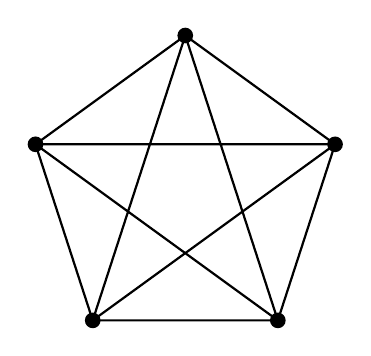
\begin{tikzpicture}
		\draw[thick,black]  (18:2) \foreach \a in {90,162,234,306} { -- (\a:2) } -- cycle;
		\draw[thick,black] (18:2) \foreach \a in {162,306,90,234} { -- (\a:2) } -- cycle;
		\foreach \a in {18,90,162,234,306} { \node[black,fill=black,circle,inner sep=2pt] at (\a:2){}; }
	\end{tikzpicture}
	\caption{完全图}
\end{figure}

\vspace{0.5cm}

\subsection{圈图(Cycle Graph)}

圈图是由$ n\ (n \ge 3) $的顶点,及边$ (v_1, v_2) $、$ (v_2, v_3) $、$ (v_{n-1}, v_n) $、$ (v_n, v_1) $组成的简单图。

\begin{figure}[H]
	\centering
	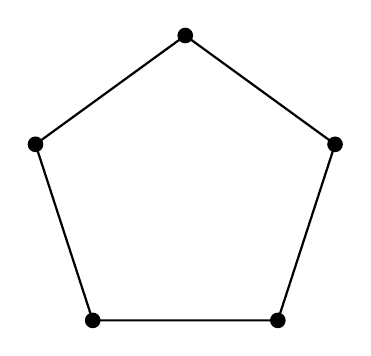
\begin{tikzpicture}
		\draw[thick,black]  (18:2) \foreach \a in {90,162,234,306} { -- (\a:2) } -- cycle;
		\foreach \a in {18,90,162,234,306} { \node[black,fill=black,circle,inner sep=2pt] at (\a:2){}; }
	\end{tikzpicture}
	\caption{圈图}
\end{figure}

\vspace{0.5cm}

\subsection{n立方图}

n立方图记作$ Q_n $,是用顶点表示$ 2^n $个长度为n的二进制串的图。n立方图的两个顶点相邻,当且仅当它们所表示的二进制串恰有一位不同。\\

\begin{figure}[H]
	\centering
	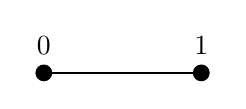
\begin{tikzpicture}
		\node[draw, black, fill=black, circle, inner sep=2pt, label=above:0] at (0,0){};
		\node[draw, black, fill=black, circle, inner sep=2pt, label=above:1] at (2,0){};
		\draw[black, thick] (0,0) -- (2,0);
	\end{tikzpicture}
	\caption{$ Q_1 $}
\end{figure}

\begin{figure}[H]
	\centering
	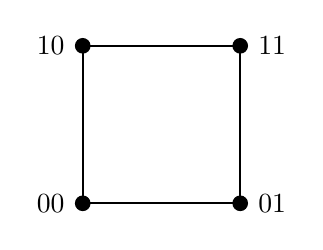
\begin{tikzpicture}
		\node[black, fill=black, circle, inner sep=2pt, label=left:00] at (0,0){};
		\node[black, fill=black, circle, inner sep=2pt, label=right:01] at (2,0){};
		\node[black, fill=black, circle, inner sep=2pt, label=right:11] at (2,2){};
		\node[black, fill=black, circle, inner sep=2pt, label=left:10] at (0,2){};
		\draw[black, thick] (0,0) -- (2,0) -- (2,2) -- (0,2) -- (0,0);
	\end{tikzpicture}
	\caption{$ Q_2 $}
\end{figure}

\begin{figure}[H]
	\centering
	\begin{tikzpicture}
		\node[black, fill=black, circle, inner sep=2pt, label=left:000] at (0,0){};
		\node[black, fill=black, circle, inner sep=2pt, label=right:100] at (2,0){};
		\node[black, fill=black, circle, inner sep=2pt, label=right:110] at (2,2){};
		\node[black, fill=black, circle, inner sep=2pt, label=left:010] at (0,2){};
		\draw[black, thick] (0,0) -- (2,0) -- (2,2) -- (0,2) -- (0,0);

		\node[black, fill=black, circle, inner sep=2pt, label=left:001] at (0.8,0.8){};
		\node[black, fill=black, circle, inner sep=2pt, label=right:101] at (2.8,0.8){};
		\node[black, fill=black, circle, inner sep=2pt, label=right:111] at (2.8,2.8){};
		\node[black, fill=black, circle, inner sep=2pt, label=left:011] at (0.8,2.8){};
		\draw[black, thick] (0.8,0.8) -- (2.8,0.8) -- (2.8,2.8) -- (0.8,2.8) -- (0.8,0.8);

		\draw[black, thick] (0,0) -- (0.8,0.8);
		\draw[black, thick] (0,2) -- (0.8,2.8);
		\draw[black, thick] (2,2) -- (2.8,2.8);
		\draw[black, thick] (2,0) -- (2.8,0.8);
	\end{tikzpicture}
	\caption{$ Q_3 $}
\end{figure}

\vspace{0.5cm}

\subsection{二分图(Bipartite Graph)}

二分图是指图的顶点可以分成两个不相交的子集,使得每条边都连接一个子集中的顶点与另一个子集中的顶点。\\

如果能够对图中的顶点赋予两种不同的颜色,并且使得没有两个相邻的顶点的颜色是一样的,那么这个图是一个二分图。

\begin{figure}[H]
	\centering
	\begin{tikzpicture}
		\node[red, fill=red, circle, inner sep=2pt] at (0,0){};
		\node[black, fill=black, circle, inner sep=2pt] at (2,0){};
		\node[black, fill=black, circle, inner sep=2pt] at (0,2){};
		\node[black, fill=black, circle, inner sep=2pt] at (2,2){};
		\node[red, fill=red, circle, inner sep=2pt] at (1,3){};
		\node[black, fill=black, circle, inner sep=2pt] at (3,3){};
		\node[red, fill=red, circle, inner sep=2pt] at (3,1){};
		\draw[black, thick] (2,0) -- (0,0) -- (0,2) -- (1,3) -- (3,3) -- (3,1) -- (0,2);
		\draw[black, thick] (0,0) -- (2,2) -- (1,3);
	\end{tikzpicture}
	\caption{二分图}
\end{figure}

\begin{figure}[H]
	\centering
	\begin{tikzpicture}
		\node[black, fill=black, circle, inner sep=2pt] at (0,0){};
		\node[red, fill=red, circle, inner sep=2pt] at (2,1.5){};
		\node[red, fill=red, circle, inner sep=2pt] at (2,-1.5){};
		\node[black, fill=black, circle, inner sep=2pt] at (4,1.5){};
		\node[black, fill=black, circle, inner sep=2pt] at (4,-1.5){};
		\node[red, fill=red, circle, inner sep=2pt] at (6,0){};
		\draw[black, thick] (0,0) -- (2,1.5) -- (4,1.5) -- (6,0) -- (4,-1.5) -- (2,-1.5) -- (0,0);
	\end{tikzpicture}
	\caption{二分图}
\end{figure}

\begin{figure}[H]
	\centering
	\begin{tikzpicture}
		\node[red, fill=red, circle, inner sep=2pt] at (0,1.5){};
		\node[red, fill=red, circle, inner sep=2pt] at (0,3){};
		\node[red, fill=red, circle, inner sep=2pt] at (0,4.5){};
		\node[black, fill=black, circle, inner sep=2pt] at (2,0){};
		\node[black, fill=black, circle, inner sep=2pt] at (2,1.5){};
		\node[black, fill=black, circle, inner sep=2pt] at (2,3){};
		\node[black, fill=black, circle, inner sep=2pt] at (2,4.5){};
		\draw[black, thick] (0,1.5) -- (2,0);
		\draw[black, thick] (0,1.5) -- (2,3);
		\draw[black, thick] (0,1.5) -- (2,4.5);
		\draw[black, thick] (0,3) -- (2,0);
		\draw[black, thick] (0,3) -- (2,4.5);
		\draw[black, thick] (0,4.5) -- (2,1.5);
		\draw[black, thick] (0,4.5) -- (2,3);
		\draw[black, thick] (0,4.5) -- (2,4.5);
	\end{tikzpicture}
	\caption{二分图}
\end{figure}

其中第一和第三个图是同构的,但是第三个图可以更加明显地看出是二分图。\\

如果一个图中存在经过奇数个顶点的环路,那么这个图一定不是二分图。

\begin{figure}[H]
	\centering
	\begin{tikzpicture}
		\draw[thick,black]  (18:2) \foreach \a in {90,162,234,306} { -- (\a:2) } -- cycle;
		\foreach \a in {18,90,162,234,306} { \node[black,fill=black,circle,inner sep=2pt] at (\a:2){}; }
	\end{tikzpicture}
	\caption{非二分图}
\end{figure}

\vspace{0.5cm}

\subsection{同构(Isomorphsim)}

对于同一个图,可以画成各种不同的样子,但都具有相同数目的边、相同数目的顶点,它们有着一一对应的关系,对应的顶点具有相同的连接性。这些图的不同形式称之为图的同构。\\

假设$ G_1 = (V1_1, E_1) $和$ G_2 = (V_2, E_2) $是简单图,若存在从$ V_1 $到$ V_2 $的一一对应函数$ f $,且对于所有$ (u, v) \in E_1 $,都满足$ (f(u), f(v)) \in E_2 $,则称$ G_1 $和$ G_2 $是同构的。

\begin{tcolorbox}
	\mybox{Exercise}
	\begin{figure}[H]
		\centering
		\begin{tikzpicture}
			\node[black, fill=black, circle, inner sep=2pt, label=left:c] at (0,0){};
			\node[black, fill=black, circle, inner sep=2pt, label=right:d] at (2,0){};
			\node[black, fill=black, circle, inner sep=2pt, label=right:b] at (2,2){};
			\node[black, fill=black, circle, inner sep=2pt, label=left:a] at (0,2){};
			\draw[black, thick] (0,0) -- (2,2) -- (2,0) -- (0,2) -- (0,0);
		\end{tikzpicture}

		\begin{tikzpicture}
			\node[black, fill=black, circle, inner sep=2pt, label=left:y] at (1,0){};
			\node[black, fill=black, circle, inner sep=2pt, label=right:x] at (2,1){};
			\node[black, fill=black, circle, inner sep=2pt, label=right:w] at (1,2){};
			\node[black, fill=black, circle, inner sep=2pt, label=left:z] at (0,1){};
			\draw[black, thick] (1,0) -- (2,1) -- (1,2) -- (0,1) -- (1,0);
		\end{tikzpicture}
	\end{figure}

	\vspace{-1cm}

	\begin{align*}
		f(a)         & = w      \\
		f(b)         & = y      \\
		f(c)         & = z      \\
		f(d)         & = x      \\
		(f(a), f(d)) & = (w, x)
	\end{align*}
\end{tcolorbox}

\newpage

\section{图的遍历}

\subsection{深度优先搜索(DFS, Depth First Search)}

深度优先搜索是一种一头扎到底的遍历方法,选择一条路,尽可能不断地深入,遇到死路就回退,回退过程中如果遇到没探索的支路,就进入该支路继续深入。\\

例如一个小镇的每个地点都藏有可以实现愿望的光玉,现在要从0号出生点出发去收集所有的光玉。

\begin{figure}[H]
	\centering
	\begin{tikzpicture}
		\begin{scope}[every node/.style={circle,thick,draw}]
			\node (0) at (2.5,4) {0};
			\node (1) at (5,3) {1};
			\node (2) at (2.5,2) {2};
			\node (3) at (1,0) {3};
			\node (4) at (3,0) {4};
			\node (5) at (5,1) {5};
			\node (6) at (6,-1) {6};
			\node (7) at (0,3) {7};
		\end{scope}

		\begin{scope}[>={Stealth[black]},
			every node/.style={},
			every edge/.style={draw=black,very thick}]
			\path [-] (0) edge node {} (1);
			\path [-] (0) edge node {} (2);
			\path [-] (0) edge node {} (7);
			\path [-] (1) edge node {} (4);
			\path [-] (1) edge node {} (5);
			\path [-] (2) edge node {} (4);
			\path [-] (3) edge node {} (4);
			\path [-] (5) edge node {} (6);
		\end{scope}
	\end{tikzpicture}
	\caption{深度优先搜索}
\end{figure}

二叉树的先序遍历本质上也可以认为是图的深度优先遍历。要想实现回溯,可以利用栈的先进后出的特性,也可以采用递归的方式,因为递归本身就是基于方法调用栈来实现的。

\vspace{0.5cm}

\subsection{广度优先搜索(BFS, Breath First Search)}

除了深度优先搜索一头扎到底的方法以外,还有一种方法就是首先把从源点相邻的顶点遍历,然后再遍历稍微远一点的顶点,再去遍历更远一点的顶点。\\

二叉树的层次遍历本质上也可以认为是图的广度优先遍历,需要借助队列来实现重放。

\begin{figure}[H]
	\centering
	\begin{tikzpicture}[
			level distance=1.5cm,
			level 1/.style={sibling distance=4cm},
			level 2/.style={sibling distance=2cm},
			level 3/.style={sibling distance=1cm}
		]
		\node[circle,draw] {1}
		child {
				node[circle,draw] {2}
				child {
						node[circle,draw] {4}
						child {node[circle,draw] {8}}
						child {node[circle,draw] {9}}
					}
				child {
						node[circle,draw] {5}
						child {node[circle,draw] {10}}
						child {node[circle,draw] {11}}
					}
			}
		child {
				node[circle,draw] {3}
				child {
						node[circle,draw] {6}
						child {node[circle,draw] {12}}
						child {node[circle,draw] {13}}
					}
				child {
						node[circle,draw] {7}
						child {node[circle,draw] {14}}
						child {node[circle,draw] {15}}
					}
			};
	\end{tikzpicture}
\end{figure}

\begin{figure}[H]
	\centering
	\begin{tikzpicture}
		\begin{scope}[every node/.style={circle,thick,draw}]
			\node (1) at (0,0) {1};
			\node (2) at (-1,1) {2};
			\node (3) at (1,1) {3};
			\node (4) at (1.5,0) {4};
			\node (5) at (1,-1) {5};
			\node (6) at (-1,-1) {6};
			\node (7) at (-1.5,0) {7};
			\node (8) at (-2,2) {8};
			\node (9) at (-0.5,2) {9};
			\node (10) at (2,2) {10};
			\node (11) at (2.5,1) {11};
			\node (12) at (3,0) {12};
			\node (13) at (2.5,-1) {13};
			\node (14) at (2,-2) {14};
			\node (15) at (0,-2) {15};
			\node (16) at (-2,-2) {16};
			\node (17) at (-2.5,-1) {17};
			\node (18) at (-3,0) {18};
			\node (19) at (-2.5,1) {19};
		\end{scope}

		\begin{scope}[>={Stealth[black]},
			every node/.style={},
			every edge/.style={draw=black,very thick}]
			\path [-] (1) edge node {} (2);
			\path [-] (1) edge node {} (3);
			\path [-] (1) edge node {} (4);
			\path [-] (1) edge node {} (5);
			\path [-] (1) edge node {} (6);
			\path [-] (1) edge node {} (7);
			\path [-] (2) edge node {} (8);
			\path [-] (2) edge node {} (9);
			\path [-] (3) edge node {} (10);
			\path [-] (4) edge node {} (11);
			\path [-] (4) edge node {} (12);
			\path [-] (4) edge node {} (13);
			\path [-] (5) edge node {} (14);
			\path [-] (5) edge node {} (15);
			\path [-] (6) edge node {} (16);
			\path [-] (7) edge node {} (17);
			\path [-] (7) edge node {} (18);
			\path [-] (7) edge node {} (19);
		\end{scope}
	\end{tikzpicture}
	\caption{广度优先搜索}
\end{figure}

\newpage

\section{连通图}

\subsection{连通图}

图还有一些有关路径的术语:

\begin{itemize}
	\item 连通:如果从顶点V到W存在一条路径,则称V和W是连通的。

	\item 路径:顶点V到W的路径是一系列顶点$ \{V, v_1, v_2, \dots, v_n, W\} $的集合,其中任意一对相邻的顶点间都有图中的边。

	\item 路径长度:路径中边的个数,如果是带权图(网络),则是所有边的权重和。

	\item 简单路径:顶点V到W之间的路径中所有顶点都不同。

	\item 回路:起点等于终点的路径。
\end{itemize}

如果图中任意两顶点均连通,那么称这个图是一个连通图。\\

一个图的连通分量指的是图的极大连通子图,极大连通子图需要满足两点要求:

\begin{enumerate}
	\item 顶点数到达极大,即再加一个顶点就不连通了。
	\item 边数达到极大,即包含子图中所有顶点相连的所有边。
\end{enumerate}

\begin{figure}[H]
	\centering
	\begin{tikzpicture}
		\begin{scope}[every node/.style={circle,thick,draw}]
			\node (A) at (0,2) {A};
			\node (B) at (-2,0) {B};
			\node (C) at (0,-2) {C};
			\node (D) at (2,0) {D};
			\node (E) at (-0.75,0) {E};
			\node (F) at (0.75,0) {F};
		\end{scope}

		\begin{scope}[>={Stealth[black]},
			every node/.style={},
			every edge/.style={draw=black,very thick}]
			\path [-] (A) edge node {} (B);
			\path [-] (B) edge node {} (C);
			\path [-] (C) edge node {} (D);
			\path [-] (D) edge node {} (A);
			\path [-] (E) edge node {} (F);
		\end{scope}
	\end{tikzpicture}
	\caption{图G}
\end{figure}

\begin{figure}[H]
	\centering
	\begin{tikzpicture}
		\begin{scope}[every node/.style={circle,thick,draw}]
			\node (A) at (0,2) {A};
			\node (B) at (-2,0) {B};
			\node (C) at (0,-2) {C};
			\node (D) at (2,0) {D};
		\end{scope}

		\begin{scope}[>={Stealth[black]},
			every node/.style={},
			every edge/.style={draw=black,very thick}]
			\path [-] (A) edge node {} (B);
			\path [-] (B) edge node {} (C);
			\path [-] (C) edge node {} (D);
			\path [-] (D) edge node {} (A);
		\end{scope}
	\end{tikzpicture}
	\caption{是图G的极大连通子图}
\end{figure}

\begin{figure}[H]
	\centering
	\begin{tikzpicture}
		\begin{scope}[every node/.style={circle,thick,draw}]
			\node (E) at (-0.75,0) {E};
			\node (F) at (0.75,0) {F};
		\end{scope}

		\begin{scope}[>={Stealth[black]},
			every node/.style={},
			every edge/.style={draw=black,very thick}]
			\path [-] (E) edge node {} (F);
		\end{scope}
	\end{tikzpicture}
	\caption{是图G的极大连通子图}
\end{figure}

\begin{figure}[H]
	\centering
	\begin{tikzpicture}
		\begin{scope}[every node/.style={circle,thick,draw}]
			\node (A) at (0,2) {A};
			\node (B) at (-2,0) {B};
			\node (C) at (0,-2) {C};
			\node (D) at (2,0) {D};
		\end{scope}

		\begin{scope}[>={Stealth[black]},
			every node/.style={},
			every edge/.style={draw=black,very thick}]
			\path [-] (A) edge node {} (B);
			\path [-] (C) edge node {} (D);
			\path [-] (D) edge node {} (A);
		\end{scope}
	\end{tikzpicture}
	\caption{不是图G的极大连通子图}
\end{figure}

\begin{figure}[H]
	\centering
	\begin{tikzpicture}
		\begin{scope}[every node/.style={circle,thick,draw}]
			\node (B) at (-2,0) {B};
			\node (C) at (0,-2) {C};
			\node (D) at (2,0) {D};
		\end{scope}

		\begin{scope}[>={Stealth[black]},
			every node/.style={},
			every edge/.style={draw=black,very thick}]
			\path [-] (B) edge node {} (C);
			\path [-] (C) edge node {} (D);
		\end{scope}
	\end{tikzpicture}
	\caption{不是图G的极大连通子图}
\end{figure}

对于有向图而言,如果有向图中任意一对顶点V和W之间存在双向路径,既可以从$ V $走到$ W $,也可以从$ W $走到$ V $,但这两条路径不一定是同一条,则称该图为强连通图。\\

如果有向图不是强连通图,但将所有的有向边替换为无向边之后可以变为连通图,则称该图为弱连通图。\\

有向图的极大强连通子图称为强连通分量。\\

\begin{figure}[H]
	\centering
	\begin{tikzpicture}
		\begin{scope}[every node/.style={circle,thick,draw}]
			\node (A) at (0,2) {A};
			\node (B) at (-2,0) {B};
			\node (C) at (0,-2) {C};
			\node (D) at (2,0) {D};
		\end{scope}

		\begin{scope}[>={Stealth[black]},
			every node/.style={},
			every edge/.style={draw=black,very thick}]
			\path [->] (A) edge node {} (B);
			\path [->] (B) edge node {} (C);
			\path [->] (C) edge node {} (A);
			\path [->] (A) edge node {} (D);
		\end{scope}
	\end{tikzpicture}
	\caption{有向图G}
\end{figure}

\begin{figure}[H]
	\centering
	\begin{tikzpicture}
		\begin{scope}[every node/.style={circle,thick,draw}]
			\node (A) at (0,2) {A};
			\node (B) at (-2,0) {B};
			\node (C) at (0,-2) {C};
		\end{scope}

		\begin{scope}[>={Stealth[black]},
			every node/.style={},
			every edge/.style={draw=black,very thick}]
			\path [->] (A) edge node {} (B);
			\path [->] (B) edge node {} (C);
			\path [->] (C) edge node {} (A);
		\end{scope}
	\end{tikzpicture}
	\caption{是有向图G的强连通分量}
\end{figure}

\begin{figure}[H]
	\centering
	\begin{tikzpicture}
		\begin{scope}[every node/.style={circle,thick,draw}]
			\node (D) at (2,0) {D};
		\end{scope}
	\end{tikzpicture}
	\caption{是有向图G的强连通分量}
\end{figure}

\newpage

\section{最短路径}

\subsection{最短路径(Shortest Path)}

在现实中很多需要都运用到了最短路径的算法,例如从一个地铁站到另一个地铁站的最快换乘路线等。地铁线路图中,地铁站可以看作是图的顶点,站与站之间的线路可以看作是边,权重可以是距离、时间、费用等。\\

\begin{figure}[H]
	\centering
	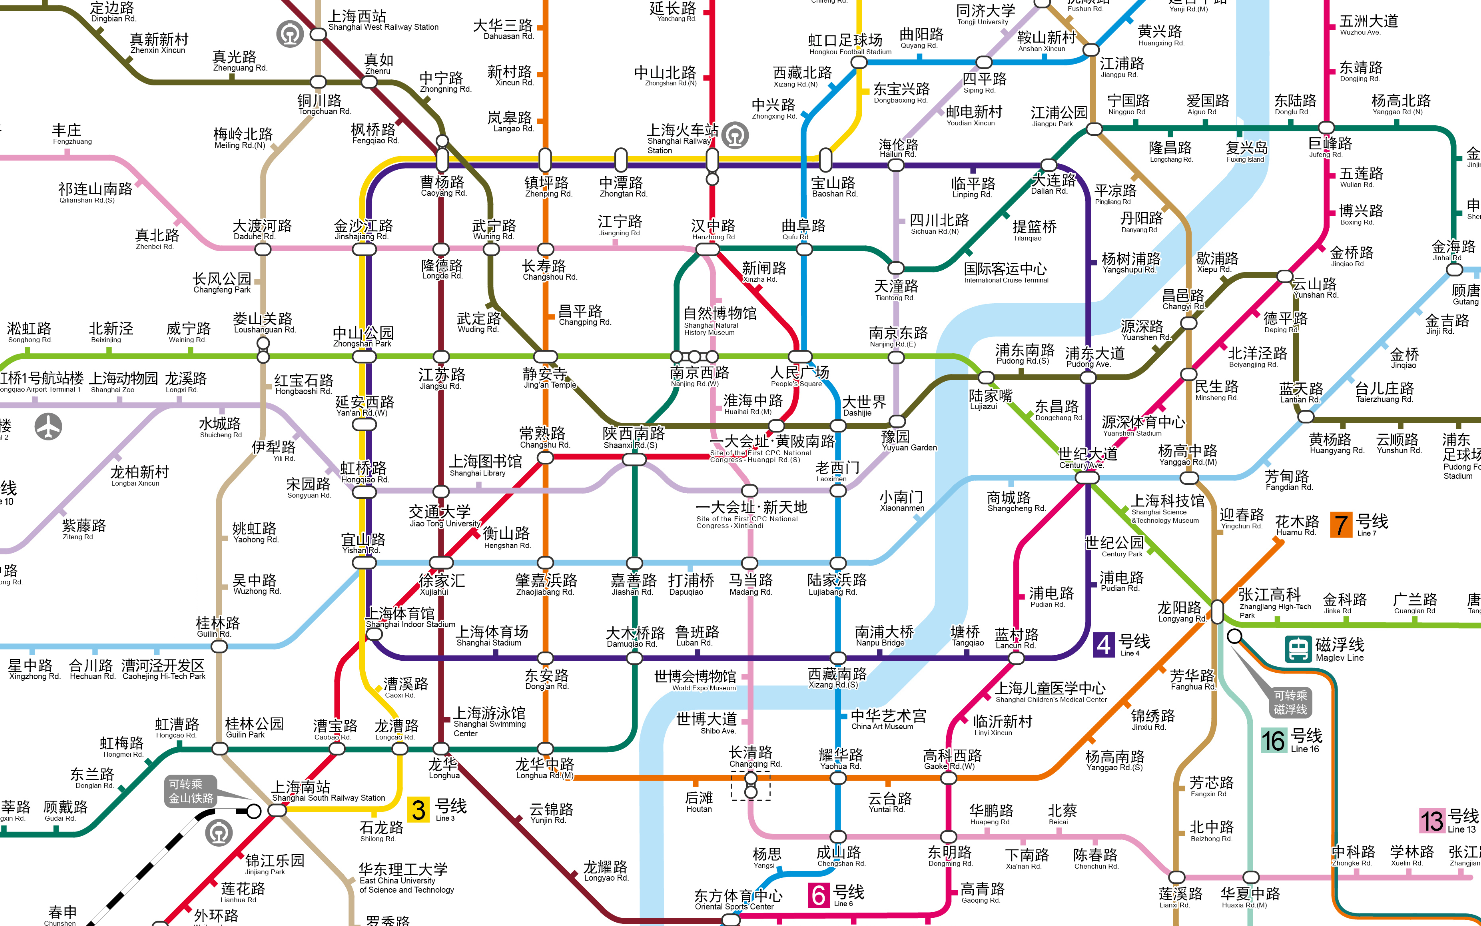
\includegraphics[scale=0.3]{img/Chapter8/8-6/1.png}
	\caption{上海地铁线路图}
\end{figure}

在网络中,求两个不同顶点之间的所有路径中,边的权值之和最小的那一条路径,这条路径就是两点之间的最短路径。其中最短路径的第一个顶点称为源点(source),最后一个顶点为终点(destination)。\\

图的最短路径问题分为2种类型:

\begin{enumerate}
	\item 单源最短路径:从某固定源点出发,求到所有其它顶点的最短路径。
	\item 多源最短路径:求任意两顶点间的最短路径。
\end{enumerate}

\vspace{0.5cm}

\subsection{无权图的单源最短路径算法(SSSP, Single-Source Shortest Path)}

无权图的单源最短路径算法可以按照递增(非递减)的顺序找出到各个顶点的最短路,算法类似广度优先遍历。\\

例如在一个无权图中,以顶点3作为源点,离源点距离为1的顶点有1和6,距离为2的顶点有2和4,距离为3的顶点有5和7。

\begin{figure}[H]
	\centering
	\begin{tikzpicture}
		\begin{scope}[every node/.style={circle,thick,draw}]
			\node (1) at (-1.5,2) {1};
			\node (2) at (1.5,2) {2};
			\node (3) at (-4,0) {3};
			\node (4) at (0,0) {4};
			\node (5) at (4,0) {5};
			\node (6) at (-1.5,-2) {6};
			\node (7) at (1.5,-2) {7};
		\end{scope}

		\begin{scope}[>={Stealth[black]},
			every node/.style={},
			every edge/.style={draw=black,very thick}]
			\path [->] (1) edge node {} (2);
			\path [->] (1) edge node {} (4);
			\path [->] (2) edge node {} (4);
			\path [->] (2) edge node {} (5);
			\path [->] (3) edge node {} (1);
			\path [->] (3) edge node {} (6);
			\path [->] (4) edge node {} (3);
			\path [->] (4) edge node {} (5);
			\path [->] (4) edge node {} (6);
			\path [->] (4) edge node {} (7);
			\path [->] (5) edge node {} (7);
			\path [->] (7) edge node {} (6);
		\end{scope}
	\end{tikzpicture}
\end{figure}

无权图的单元最短路径算法中,dist[v]存储从源点S到v的最短路径,初始化源点dist[S]的距离为0,path[v]表示达到顶点路径v上一个经过的顶点。

\begin{table}[H]
	\centering
	\setlength{\tabcolsep}{5mm}{
		\begin{tabular}{|c|c|c|c|c|c|c|c|}
			\hline
			\textbf{顶点} & \textbf{1} & \textbf{2} & \textbf{3} & \textbf{4} & \textbf{5} & \textbf{6} & \textbf{7} \\
			\hline
			\textbf{dist} & 1          & 2          & 0          & 2          & 3          & 1          & 3          \\
			\hline
			\textbf{path} & 3          & 1          & -1         & 1          & 2          & 3          & 4          \\
			\hline
		\end{tabular}
	}
	\caption{最短路径表}
\end{table}

\vspace{0.5cm}

\subsection{有权图的单源最短路径算法}

有权图的最短路径不一定是经过顶点树最少的路。如果图中存在负值圈(negative-cost cycle)的话会导致算法失效,因为沿着回路走无穷多次,花销是负无穷。

\begin{figure}[H]
	\centering
	\begin{tikzpicture}
		\begin{scope}[every node/.style={circle,thick,draw}]
			\node (1) at (-1.5,2) {1};
			\node (2) at (1.5,2) {2};
			\node (3) at (-4,0) {3};
			\node (4) at (0,0) {4};
			\node (5) at (4,0) {5};
			\node (6) at (-1.5,-2) {6};
			\node (7) at (1.5,-2) {7};
		\end{scope}

		\begin{scope}[>={Stealth[black]},
			every node/.style={fill=white,circle},
			every edge/.style={draw=black,very thick}]
			\path [->] (1) edge node {2} (2);
			\path [->] (1) edge node {1} (4);
			\path [->, red] (4) edge node {3} (2);
			\path [->, red] (2) edge node {-10} (5);
			\path [->] (3) edge node {4} (1);
			\path [->] (3) edge node {5} (6);
			\path [->] (4) edge node {2} (3);
			\path [->, red] (5) edge node {2} (4);
			\path [->] (4) edge node {8} (6);
			\path [->] (4) edge node {4} (7);
			\path [->] (5) edge node {6} (7);
			\path [->] (7) edge node {1} (6);
		\end{scope}
	\end{tikzpicture}
	\caption{负值圈}
\end{figure}

带权图的单源最短路径可以通过迪杰斯特拉(Dijkstra)算法解决。\\

特斯拉?什么鬼?\\

迪杰斯特拉算法的本质是不断刷新起点与其他各个顶点之间的距离表。Dijkstra算法采用了贪心的思想,每次都未收录的顶点中选取dist值最小的收录。每当收录一个顶点时,可能会影响另外一个顶点的dist值。

\vspace{-0.5cm}

$$
	dist[w] = min\{dist[w], dist[v] + weight_{<v, w>}\}
$$

例如计算从源点A到其它各顶点的最短路径。

\begin{figure}[H]
	\centering
	\begin{tikzpicture}
		\begin{scope}[every node/.style={circle,thick,draw}]
			\node (A) at (-3,2.5) {A};
			\node (B) at (-4,0) {B};
			\node (C) at (0,3) {C};
			\node (D) at (0,0) {D};
			\node (E) at (-1.5,-2.5) {E};
			\node (F) at (2,-1) {F};
			\node (G) at (3,-3) {G};
		\end{scope}

		\begin{scope}[>={Stealth[black]},
			every node/.style={fill=white,circle},
			every edge/.style={draw=black,very thick}]
			\path [-] (A) edge node {5} (B);
			\path [-] (A) edge node {2} (C);
			\path [-] (B) edge node {1} (D);
			\path [-] (B) edge node {6} (E);
			\path [-] (C) edge node {6} (D);
			\path [-] (C) edge node {8} (F);
			\path [-] (E) edge node {1} (D);
			\path [-] (E) edge node {7} (G);
			\path [-] (F) edge node {3} (G);
		\end{scope}
	\end{tikzpicture}
\end{figure}

第1步:创建距离表。其中表中key是顶点名称,value是源点A到对应顶点的已知最短距离。一开始并不知道最短路径是多少,因此value都为$ \infty $。

\begin{table}[H]
	\centering
	\setlength{\tabcolsep}{5mm}{
		\begin{tabular}{|c|c|c|c|c|c|}
			\hline
			\textbf{B} & \textbf{C} & \textbf{D} & \textbf{E} & \textbf{F} & \textbf{G} \\
			\hline
			$ \infty $ & $ \infty $ & $ \infty $ & $ \infty $ & $ \infty $ & $ \infty $ \\
			\hline
		\end{tabular}
	}
\end{table}

第2步:找到源点A的邻接点B和C,从A到B的距离是5,从A到C的距离是2。

\begin{table}[H]
	\centering
	\setlength{\tabcolsep}{5mm}{
		\begin{tabular}{|c|c|c|c|c|c|}
			\hline
			\textbf{B}         & \textbf{C}         & \textbf{D} & \textbf{E} & \textbf{F} & \textbf{G} \\
			\hline
			\textcolor{red}{5} & \textcolor{red}{2} & $ \infty $ & $ \infty $ & $ \infty $ & $ \infty $ \\
			\hline
		\end{tabular}
	}
\end{table}

第3步:从距离表中找到从A出发距离最短的顶点,也就是顶点C。找到顶点C的邻接点D和F(A已经遍历过不需要考虑)。从C到D的距离是6,所以从A到D的距离是2 + 6 = 8;从C到F的距离是8,所以从A到F的距离是2 + 8 = 10。

\begin{table}[H]
	\centering
	\setlength{\tabcolsep}{5mm}{
		\begin{tabular}{|c|c|c|c|c|c|}
			\hline
			\textbf{B} & \textbf{C} & \textbf{D}         & \textbf{E} & \textbf{F}          & \textbf{G} \\
			\hline
			5          & 2          & \textcolor{red}{8} & $ \infty $ & \textcolor{red}{10} & $ \infty $ \\
			\hline
		\end{tabular}
	}
\end{table}

第4步:从距离表中找到从A出发距离最短的顶点(C已经遍历过不需要考虑),也就是顶点B。找到顶点B的邻接点D和E(A已经遍历过不需要考虑)。从B到D的距离是1,所以从A到D的距离是5 + 1 = 6,小于距离表中的8;从B到E的距离是6,所以从A到E的距离是5 + 6 = 11。

\begin{table}[H]
	\centering
	\setlength{\tabcolsep}{5mm}{
		\begin{tabular}{|c|c|c|c|c|c|}
			\hline
			\textbf{B} & \textbf{C} & \textbf{D}         & \textbf{E}          & \textbf{F} & \textbf{G} \\
			\hline
			5          & 2          & \textcolor{red}{6} & \textcolor{red}{11} & 10         & $ \infty $ \\
			\hline
		\end{tabular}
	}
\end{table}

第5步:从距离表中找到从A出发距离最短的顶点(B和C不用考虑),也就是顶点D。找到顶点D的邻接点E和F。从D到E的距离是1,所以从A到E的距离是6 + 1 = 7,小于距离表中的11;从D到F的距离是2,所以从A到F的距离是6 + 2 = 8,小于距离表中的10。

\begin{table}[H]
	\centering
	\setlength{\tabcolsep}{5mm}{
		\begin{tabular}{|c|c|c|c|c|c|}
			\hline
			\textbf{B} & \textbf{C} & \textbf{D} & \textbf{E}         & \textbf{F}         & \textbf{G} \\
			\hline
			5          & 2          & 6          & \textcolor{red}{7} & \textcolor{red}{8} & $ \infty $ \\
			\hline
		\end{tabular}
	}
\end{table}

第6步:从距离表中找到从A出发距离最短的顶点,也就是顶点E。找到顶点E的邻接点G。从E到G的距离是7,所以从A到G的距离是7 + 7 = 14。

\begin{table}[H]
	\centering
	\setlength{\tabcolsep}{5mm}{
		\begin{tabular}{|c|c|c|c|c|c|}
			\hline
			\textbf{B} & \textbf{C} & \textbf{D} & \textbf{E} & \textbf{F} & \textbf{G}          \\
			\hline
			5          & 2          & 6          & 7          & 8          & \textcolor{red}{14} \\
			\hline
		\end{tabular}
	}
\end{table}

第7步:从距离表中找到从A出发距离最短的顶点,也就是顶点F。找到顶点F的邻接点G。从F到G的距离是3,所以从A到G的距离是8 + 3 = 11,小于距离表中的14。

\begin{table}[H]
	\centering
	\setlength{\tabcolsep}{5mm}{
		\begin{tabular}{|c|c|c|c|c|c|}
			\hline
			\textbf{B} & \textbf{C} & \textbf{D} & \textbf{E} & \textbf{F} & \textbf{G}          \\
			\hline
			5          & 2          & 6          & 7          & 8          & \textcolor{red}{11} \\
			\hline
		\end{tabular}
	}
\end{table}

最终,距离表中存储的是从源点A到所有顶点的最短距离。\\

\subsection{多源最短路径算法}

如何能够求出一个带权图中所有顶点两两之间的最短距离呢?\\

对了!刚刚学过了Dijkstra算法,可以对每个顶点都使用一次Dijkstra算法,这样就求出了所有顶点之间的最短距离。\\

这个思路确实可以实现,但是Dijkstra算法的代码逻辑比较复杂,有没有更简单的方法呢?\\

弗洛伊德(Floyd-Warshall)算法是专门用于寻找带权图中多源点之间的最短路径算法。Floyd算法的思想是,若想缩短两点间的距离,仅有一种方式,那就是通过第三顶点绕行。\\

假设$ D^k[i][j] $为路径$ \{i \rightarrow \{l \le k\} \rightarrow j\} $的最小长度。当$ D^{k-1} $已经完成,递推到$ D^k $时:

\begin{enumerate}
	\item 如果$ k \notin \text{最短路径}\{i \rightarrow \{l \le k\} \rightarrow j\} $,则$ D^k = D^{k-1} $。
	\item 如果$ k \in \text{最短路径}\{i \rightarrow \{l \le k\} \rightarrow j\} $,该路径必定由两段最短路径组成,则$ D^k[i][j] = D^{k-1}[i][k] + D^{k-1}[k][j] $。
\end{enumerate}

例如,小哼准备去一些城市旅游,有些城市之间有公路,有些城市之间则没有。为了节省经费以及方便计划旅程,小哼希望在出发之前直到任意两个城市之间的最短路程。\\

如果要让任意两点之间的路程变短,只能引入第三个点,并通过这个顶点中转才有可能缩短原来的路程。这个中转的顶点甚至有时候不只通过一个顶点,而是经过两个或更多点中转会更短。\\

当任意两点之间不允许经过第三个点中转时,这些城市之间的最短路径就是邻接矩阵的初始路径。

\begin{figure}[H]
	\centering
	\begin{tikzpicture}
		\draw (0,0) circle(0.5) node{A};
		\draw (4,0) circle(0.5) node{B};
		\draw (4,4) circle(0.5) node{C};
		\draw (0,4) circle(0.5) node{D};

		\draw[->] (0.5,0) -- (2,0) node[below]{2} -- (3.5,0);
		\draw[->] (0.4,0.25) to[bend right] (3.75,3.6);
		\draw (3,1.5) node{6};
		\draw[->] (3.6,3.75) to[bend right] (0.25,0.4);
		\draw (1,2.5) node{7};
		\draw[->] (0,0.5) -- (0,2) node[left]{4} -- (0,3.5);
		\draw[->] (4,0.5) -- (4,2) node[right]{3} -- (4,3.5);
		\draw[->] (3.5,4) -- (2,4) node[above]{1} -- (0.5,4);
		\draw[->] (-0.5,4) to[bend right] (-0.5,0);
		\draw (-1.5,2) node{5};
		\draw[->] (0,4.5) to[bend left] (4,4.5);
		\draw (2,5.5) node{12};
	\end{tikzpicture}
\end{figure}

\begin{table}[H]
	\centering
	\setlength{\tabcolsep}{5mm}{
		\begin{tabular}{|c|c|c|c|c|}
			\hline
			           & \textbf{A} & \textbf{B} & \textbf{C} & \textbf{D} \\
			\hline
			\textbf{A} & 0          & 2          & 6          & 4          \\
			\hline
			\textbf{B} & $ \infty $ & 0          & 3          & $ \infty $ \\
			\hline
			\textbf{C} & 7          & $ \infty $ & 0          & 1          \\
			\hline
			\textbf{D} & 5          & $ \infty $ & 12         & 0          \\
			\hline
		\end{tabular}
	}
\end{table}

在只允许经过1号顶点中转的情况下,任意两点之间的最短路程更新为:

\begin{table}[H]
	\centering
	\setlength{\tabcolsep}{5mm}{
		\begin{tabular}{|c|c|c|c|c|}
			\hline
			           & \textbf{A} & \textbf{B}         & \textbf{C}          & \textbf{D} \\
			\hline
			\textbf{A} & 0          & 2                  & 6                   & 4          \\
			\hline
			\textbf{B} & $ \infty $ & 0                  & 3                   & $ \infty $ \\
			\hline
			\textbf{C} & 7          & \textcolor{red}{9} & 0                   & 1          \\
			\hline
			\textbf{D} & 5          & \textcolor{red}{7} & \textcolor{red}{11} & 0          \\
			\hline
		\end{tabular}
	}
\end{table}

在只允许经过1号和2号顶点中转的情况下,任意两点之间的最短路程更新为:

\begin{table}[H]
	\centering
	\setlength{\tabcolsep}{5mm}{
		\begin{tabular}{|c|c|c|c|c|}
			\hline
			           & \textbf{A} & \textbf{B} & \textbf{C}          & \textbf{D} \\
			\hline
			\textbf{A} & 0          & 2          & \textcolor{red}{5}  & 4          \\
			\hline
			\textbf{B} & $ \infty $ & 0          & 3                   & $ \infty $ \\
			\hline
			\textbf{C} & 7          & 9          & 0                   & 1          \\
			\hline
			\textbf{D} & 5          & 7          & \textcolor{red}{10} & 0          \\
			\hline
		\end{tabular}
	}
\end{table}

在只允许经过1号、2号和3号顶点中转的情况下,任意两点之间的最短路程更新为:

\begin{table}[H]
	\centering
	\setlength{\tabcolsep}{5mm}{
		\begin{tabular}{|c|c|c|c|c|}
			\hline
			           & \textbf{A}          & \textbf{B} & \textbf{C} & \textbf{D}         \\
			\hline
			\textbf{A} & 0                   & 2          & 5          & 4                  \\
			\hline
			\textbf{B} & \textcolor{red}{10} & 0          & 3          & \textcolor{red}{4} \\
			\hline
			\textbf{C} & 7                   & 9          & 0          & 1                  \\
			\hline
			\textbf{D} & 5                   & 7          & 10         & 0                  \\
			\hline
		\end{tabular}
	}
\end{table}

最后允许通过所有顶点作为中转,任意两点之间的最短路程更新为:

\begin{table}[H]
	\centering
	\setlength{\tabcolsep}{5mm}{
		\begin{tabular}{|c|c|c|c|c|}
			\hline
			           & \textbf{A}         & \textbf{B}         & \textbf{C} & \textbf{D} \\
			\hline
			\textbf{A} & 0                  & 2                  & 5          & 4          \\
			\hline
			\textbf{B} & \textcolor{red}{9} & 0                  & 3          & 4          \\
			\hline
			\textbf{C} & \textcolor{red}{6} & \textcolor{red}{8} & 0          & 1          \\
			\hline
			\textbf{D} & 5                  & 7                  & 10         & 0          \\
			\hline
		\end{tabular}
	}
\end{table}

\newpage

\section{最小生成树}

\subsection{最小生成树(MST, Mininum Spanning Tree)}

所谓最小生成树,就是一个图的极小连通子图,它包含原图的所有顶点,并且所有边的权值之和尽可能小。\\

最小生成树需要满足3个条件:

\begin{enumerate}
	\item 是一棵树:树不能有回路,并且$ |V| $个顶点一定有$ |V| - 1 $条边。

	\item 是生成树:包含原图的全部顶点,树的$ |V| - 1 $条边都必须在图里,并且如果向生成树中任意加一条边都一定构成回路。

	\item 边的权重和最小。
\end{enumerate}

如果最小生成树存在,那么图一定连通,反之亦然。\\

例如一个带权图,蓝色边可以把所有顶点连接起来,又保证边的权值和最小。

\begin{figure}[H]
	\centering
	\begin{tikzpicture}
		\begin{scope}[every node/.style={circle,thick,draw}]
			\node (A) at (-1.5,2) {A};
			\node (B) at (1.5,2) {B};
			\node (C) at (-4,0) {C};
			\node (D) at (0,0) {D};
			\node (E) at (4,0) {E};
			\node (F) at (-1.5,-2) {F};
		\end{scope}

		\begin{scope}[>={Stealth[black]},
			every node/.style={fill=white,circle},
			every edge/.style={draw=black,very thick}]
			\path [->] (B) edge node {7} (E);
			\path [->] (C) edge node {5} (D);
			\path [->] (F) edge node {9} (E);
		\end{scope}

		\begin{scope}[>={Stealth[blue]},
			every node/.style={fill=white,circle},
			every edge/.style={draw=blue,very thick}]
			\path [->] (A) edge node {4} (B);
			\path [->] (A) edge node {3} (C);
			\path [->] (A) edge node {1} (D);
			\path [->] (D) edge node {2} (F);
			\path [->] (D) edge node {3} (E);
		\end{scope}
	\end{tikzpicture}
\end{figure}

\begin{figure}[H]
	\centering
	\begin{tikzpicture}[
			level distance=1.5cm,
			level 1/.style={sibling distance=2cm},
			level 2/.style={sibling distance=1.5cm},
			level 3/.style={sibling distance=1cm}
		]
		\node[circle,draw] {A}
		child {node[circle,draw] {B}}
		child {node[circle,draw] {C}}
		child {
				node[circle,draw] {D}
				child {node[circle,draw] {E}}
				child {node[circle,draw] {F}}
			};
	\end{tikzpicture}
	\caption{最小生成树}
\end{figure}

图的最小生成树不是唯一的,同一个图有可能对应多个最小生成树。\\

最小生成树在现实中很很多用处。假如要在若干个城市之间铺设铁路,而预算又是有限的,那么就需要寻找成本最低的铺设方式。城市之间的交通网就像一个连通图,其实并不需要在每两个城市之间都直接进行连接,只需要一个最小生成树,保证所有的城市都有铁路可以达到即可。\\

\subsection{Prim}

Prim算法是以图的顶点为基础,从一个初始顶点开始,寻找达到其它顶点权值最小的边,并把该顶点加入到已触达顶点的集合中。当全部顶点都加入到集合时,算法的工作就完成了。Prim算法的本质是基于贪心算法(greedy algorithm)。\\

Prim算法可以理解为让一棵小树长大,每次找能够向外生长的最小边。\\

例如使用Prim算法获得一个带权图的最小生成树:

\begin{figure}[H]
	\centering
	\begin{tikzpicture}
		\begin{scope}[every node/.style={circle,thick,draw}]
			\node (A) at (-1.5,2) {A};
			\node (B) at (1.5,2) {B};
			\node (C) at (-4,0) {C};
			\node (D) at (0,0) {D};
			\node (E) at (4,0) {E};
			\node (F) at (-1.5,-2) {F};
			\node (G) at (1.5,-2) {G};
		\end{scope}

		\begin{scope}[>={Stealth[black]},
			every node/.style={fill=white,circle},
			every edge/.style={draw=black,very thick}]
			\path [-] (A) edge node {2} (B);
			\path [-] (A) edge node {1} (D);
			\path [-] (B) edge node {3} (D);
			\path [-] (B) edge node {10} (E);
			\path [-] (C) edge node {4} (A);
			\path [-] (C) edge node {5} (F);
			\path [-] (D) edge node {2} (C);
			\path [-] (D) edge node {7} (E);
			\path [-] (D) edge node {8} (F);
			\path [-] (D) edge node {4} (G);
			\path [-] (E) edge node {6} (G);
			\path [-] (G) edge node {1} (F);
		\end{scope}
	\end{tikzpicture}
\end{figure}

\begin{figure}[H]
	\centering
	\begin{tikzpicture}
		\begin{scope}[every node/.style={circle,thick,draw}]
			\node (A) at (-1.5,2) {\textcolor{red}{A}};
			\node (B) at (1.5,2) {B};
			\node (C) at (-4,0) {C};
			\node (D) at (0,0) {D};
			\node (E) at (4,0) {E};
			\node (F) at (-1.5,-2) {F};
			\node (G) at (1.5,-2) {G};
		\end{scope}

		\begin{scope}[>={Stealth[black]},
			every node/.style={fill=white,circle},
			every edge/.style={draw=black,very thick}]
			\path [-] (A) edge node {2} (B);
			\path [-] (A) edge node {1} (D);
			\path [-] (B) edge node {3} (D);
			\path [-] (B) edge node {10} (E);
			\path [-] (C) edge node {4} (A);
			\path [-] (C) edge node {5} (F);
			\path [-] (D) edge node {2} (C);
			\path [-] (D) edge node {7} (E);
			\path [-] (D) edge node {8} (F);
			\path [-] (D) edge node {4} (G);
			\path [-] (E) edge node {6} (G);
			\path [-] (G) edge node {1} (F);
		\end{scope}
	\end{tikzpicture}
\end{figure}

\begin{figure}[H]
	\centering
	\begin{tikzpicture}
		\begin{scope}[every node/.style={circle,thick,draw}]
			\node (A) at (-1.5,2) {\textcolor{red}{A}};
			\node (B) at (1.5,2) {B};
			\node (C) at (-4,0) {C};
			\node (D) at (0,0) {\textcolor{red}{D}};
			\node (E) at (4,0) {E};
			\node (F) at (-1.5,-2) {F};
			\node (G) at (1.5,-2) {G};
		\end{scope}

		\begin{scope}[>={Stealth[black]},
			every node/.style={fill=white,circle},
			every edge/.style={draw=black,very thick}]
			\path [-] (A) edge node {2} (B);
			\path [-] (B) edge node {3} (D);
			\path [-] (B) edge node {10} (E);
			\path [-] (C) edge node {4} (A);
			\path [-] (C) edge node {5} (F);
			\path [-] (D) edge node {2} (C);
			\path [-] (D) edge node {7} (E);
			\path [-] (D) edge node {8} (F);
			\path [-] (D) edge node {4} (G);
			\path [-] (E) edge node {6} (G);
			\path [-] (G) edge node {1} (F);
		\end{scope}

		\begin{scope}[>={Stealth[red]},
			every node/.style={fill=white,circle},
			every edge/.style={draw=red,very thick}]
			\path [-] (A) edge node {1} (D);
		\end{scope}
	\end{tikzpicture}
\end{figure}

\begin{figure}[H]
	\centering
	\begin{tikzpicture}
		\begin{scope}[every node/.style={circle,thick,draw}]
			\node (A) at (-1.5,2) {\textcolor{red}{A}};
			\node (B) at (1.5,2) {\textcolor{red}{B}};
			\node (C) at (-4,0) {C};
			\node (D) at (0,0) {\textcolor{red}{D}};
			\node (E) at (4,0) {E};
			\node (F) at (-1.5,-2) {F};
			\node (G) at (1.5,-2) {G};
		\end{scope}

		\begin{scope}[>={Stealth[black]},
			every node/.style={fill=white,circle},
			every edge/.style={draw=black,very thick}]
			\path [-] (B) edge node {3} (D);
			\path [-] (B) edge node {10} (E);
			\path [-] (C) edge node {4} (A);
			\path [-] (C) edge node {5} (F);
			\path [-] (D) edge node {2} (C);
			\path [-] (D) edge node {7} (E);
			\path [-] (D) edge node {8} (F);
			\path [-] (D) edge node {4} (G);
			\path [-] (E) edge node {6} (G);
			\path [-] (G) edge node {1} (F);
		\end{scope}

		\begin{scope}[>={Stealth[red]},
			every node/.style={fill=white,circle},
			every edge/.style={draw=red,very thick}]
			\path [-] (A) edge node {1} (D);
			\path [-] (A) edge node {2} (B);
		\end{scope}
	\end{tikzpicture}
\end{figure}

\begin{figure}[H]
	\centering
	\begin{tikzpicture}
		\begin{scope}[every node/.style={circle,thick,draw}]
			\node (A) at (-1.5,2) {\textcolor{red}{A}};
			\node (B) at (1.5,2) {\textcolor{red}{B}};
			\node (C) at (-4,0) {\textcolor{red}{C}};
			\node (D) at (0,0) {\textcolor{red}{D}};
			\node (E) at (4,0) {E};
			\node (F) at (-1.5,-2) {F};
			\node (G) at (1.5,-2) {G};
		\end{scope}

		\begin{scope}[>={Stealth[black]},
			every node/.style={fill=white,circle},
			every edge/.style={draw=black,very thick}]
			\path [-] (B) edge node {3} (D);
			\path [-] (B) edge node {10} (E);
			\path [-] (C) edge node {4} (A);
			\path [-] (C) edge node {5} (F);
			\path [-] (D) edge node {7} (E);
			\path [-] (D) edge node {8} (F);
			\path [-] (D) edge node {4} (G);
			\path [-] (E) edge node {6} (G);
			\path [-] (G) edge node {1} (F);
		\end{scope}

		\begin{scope}[>={Stealth[red]},
			every node/.style={fill=white,circle},
			every edge/.style={draw=red,very thick}]
			\path [-] (A) edge node {1} (D);
			\path [-] (A) edge node {2} (B);
			\path [-] (D) edge node {2} (C);
		\end{scope}
	\end{tikzpicture}
\end{figure}

\begin{figure}[H]
	\centering
	\begin{tikzpicture}
		\begin{scope}[every node/.style={circle,thick,draw}]
			\node (A) at (-1.5,2) {\textcolor{red}{A}};
			\node (B) at (1.5,2) {\textcolor{red}{B}};
			\node (C) at (-4,0) {\textcolor{red}{C}};
			\node (D) at (0,0) {\textcolor{red}{D}};
			\node (E) at (4,0) {E};
			\node (F) at (-1.5,-2) {F};
			\node (G) at (1.5,-2) {\textcolor{red}{G}};
		\end{scope}

		\begin{scope}[>={Stealth[black]},
			every node/.style={fill=white,circle},
			every edge/.style={draw=black,very thick}]
			\path [-] (B) edge node {3} (D);
			\path [-] (B) edge node {10} (E);
			\path [-] (C) edge node {4} (A);
			\path [-] (C) edge node {5} (F);
			\path [-] (D) edge node {7} (E);
			\path [-] (D) edge node {8} (F);
			\path [-] (E) edge node {6} (G);
			\path [-] (G) edge node {1} (F);
		\end{scope}

		\begin{scope}[>={Stealth[red]},
			every node/.style={fill=white,circle},
			every edge/.style={draw=red,very thick}]
			\path [-] (A) edge node {1} (D);
			\path [-] (A) edge node {2} (B);
			\path [-] (D) edge node {2} (C);
			\path [-] (D) edge node {4} (G);
		\end{scope}
	\end{tikzpicture}
\end{figure}

\begin{figure}[H]
	\centering
	\begin{tikzpicture}
		\begin{scope}[every node/.style={circle,thick,draw}]
			\node (A) at (-1.5,2) {\textcolor{red}{A}};
			\node (B) at (1.5,2) {\textcolor{red}{B}};
			\node (C) at (-4,0) {\textcolor{red}{C}};
			\node (D) at (0,0) {\textcolor{red}{D}};
			\node (E) at (4,0) {E};
			\node (F) at (-1.5,-2) {\textcolor{red}{F}};
			\node (G) at (1.5,-2) {\textcolor{red}{G}};
		\end{scope}

		\begin{scope}[>={Stealth[black]},
			every node/.style={fill=white,circle},
			every edge/.style={draw=black,very thick}]
			\path [-] (B) edge node {3} (D);
			\path [-] (B) edge node {10} (E);
			\path [-] (C) edge node {4} (A);
			\path [-] (C) edge node {5} (F);
			\path [-] (D) edge node {7} (E);
			\path [-] (D) edge node {8} (F);
			\path [-] (E) edge node {6} (G);
		\end{scope}

		\begin{scope}[>={Stealth[red]},
			every node/.style={fill=white,circle},
			every edge/.style={draw=red,very thick}]
			\path [-] (A) edge node {1} (D);
			\path [-] (A) edge node {2} (B);
			\path [-] (D) edge node {2} (C);
			\path [-] (D) edge node {4} (G);
			\path [-] (G) edge node {1} (F);
		\end{scope}
	\end{tikzpicture}
\end{figure}

\begin{figure}[H]
	\centering
	\begin{tikzpicture}
		\begin{scope}[every node/.style={circle,thick,draw}]
			\node (A) at (-1.5,2) {\textcolor{red}{A}};
			\node (B) at (1.5,2) {\textcolor{red}{B}};
			\node (C) at (-4,0) {\textcolor{red}{C}};
			\node (D) at (0,0) {\textcolor{red}{D}};
			\node (E) at (4,0) {\textcolor{red}{E}};
			\node (F) at (-1.5,-2) {\textcolor{red}{F}};
			\node (G) at (1.5,-2) {\textcolor{red}{G}};
		\end{scope}

		\begin{scope}[>={Stealth[black]},
			every node/.style={fill=white,circle},
			every edge/.style={draw=black,very thick}]
			\path [-] (B) edge node {3} (D);
			\path [-] (B) edge node {10} (E);
			\path [-] (C) edge node {4} (A);
			\path [-] (C) edge node {5} (F);
			\path [-] (D) edge node {7} (E);
			\path [-] (D) edge node {8} (F);
		\end{scope}

		\begin{scope}[>={Stealth[red]},
			every node/.style={fill=white,circle},
			every edge/.style={draw=red,very thick}]
			\path [-] (A) edge node {1} (D);
			\path [-] (A) edge node {2} (B);
			\path [-] (D) edge node {2} (C);
			\path [-] (D) edge node {4} (G);
			\path [-] (G) edge node {1} (F);
			\path [-] (E) edge node {6} (G);
		\end{scope}
	\end{tikzpicture}
\end{figure}

\vspace{0.5cm}

\subsection{Kruskal}

与Prim算法不同,Prim算法是以顶点为关键来获得最小生成树的,而Kruskal算法是以边为关键获得最小生成树的。\\

Kruskal算法可以理解为将森林合并成树,每次在图中找权值最小的边收录。\\

例如使用Kruskal算法获得一个带权图的最小生成树:

\begin{figure}[H]
	\centering
	\begin{tikzpicture}
		\begin{scope}[every node/.style={circle,thick,draw}]
			\node (A) at (-1.5,2) {\textcolor{red}{A}};
			\node (B) at (1.5,2) {B};
			\node (C) at (-4,0) {C};
			\node (D) at (0,0) {\textcolor{red}{D}};
			\node (E) at (4,0) {E};
			\node (F) at (-1.5,-2) {F};
			\node (G) at (1.5,-2) {G};
		\end{scope}

		\begin{scope}[>={Stealth[black]},
			every node/.style={fill=white,circle},
			every edge/.style={draw=black,very thick}]
			\path [-] (A) edge node {2} (B);
			\path [-] (B) edge node {3} (D);
			\path [-] (B) edge node {10} (E);
			\path [-] (C) edge node {4} (A);
			\path [-] (C) edge node {5} (F);
			\path [-] (D) edge node {2} (C);
			\path [-] (D) edge node {7} (E);
			\path [-] (D) edge node {8} (F);
			\path [-] (D) edge node {4} (G);
			\path [-] (E) edge node {6} (G);
			\path [-] (G) edge node {1} (F);
		\end{scope}

		\begin{scope}[>={Stealth[red]},
			every node/.style={fill=white,circle},
			every edge/.style={draw=red,very thick}]
			\path [-] (A) edge node {1} (D);
		\end{scope}
	\end{tikzpicture}
\end{figure}

\begin{figure}[H]
	\centering
	\begin{tikzpicture}
		\begin{scope}[every node/.style={circle,thick,draw}]
			\node (A) at (-1.5,2) {\textcolor{red}{A}};
			\node (B) at (1.5,2) {B};
			\node (C) at (-4,0) {C};
			\node (D) at (0,0) {\textcolor{red}{D}};
			\node (E) at (4,0) {E};
			\node (F) at (-1.5,-2) {\textcolor{red}{F}};
			\node (G) at (1.5,-2) {\textcolor{red}{G}};
		\end{scope}

		\begin{scope}[>={Stealth[black]},
			every node/.style={fill=white,circle},
			every edge/.style={draw=black,very thick}]
			\path [-] (A) edge node {2} (B);
			\path [-] (B) edge node {3} (D);
			\path [-] (B) edge node {10} (E);
			\path [-] (C) edge node {4} (A);
			\path [-] (C) edge node {5} (F);
			\path [-] (D) edge node {2} (C);
			\path [-] (D) edge node {7} (E);
			\path [-] (D) edge node {8} (F);
			\path [-] (D) edge node {4} (G);
			\path [-] (E) edge node {6} (G);
		\end{scope}

		\begin{scope}[>={Stealth[red]},
			every node/.style={fill=white,circle},
			every edge/.style={draw=red,very thick}]
			\path [-] (A) edge node {1} (D);
			\path [-] (G) edge node {1} (F);
		\end{scope}
	\end{tikzpicture}
\end{figure}

\begin{figure}[H]
	\centering
	\begin{tikzpicture}
		\begin{scope}[every node/.style={circle,thick,draw}]
			\node (A) at (-1.5,2) {\textcolor{red}{A}};
			\node (B) at (1.5,2) {B};
			\node (C) at (-4,0) {\textcolor{red}{C}};
			\node (D) at (0,0) {\textcolor{red}{D}};
			\node (E) at (4,0) {E};
			\node (F) at (-1.5,-2) {\textcolor{red}{F}};
			\node (G) at (1.5,-2) {\textcolor{red}{G}};
		\end{scope}

		\begin{scope}[>={Stealth[black]},
			every node/.style={fill=white,circle},
			every edge/.style={draw=black,very thick}]
			\path [-] (A) edge node {2} (B);
			\path [-] (B) edge node {3} (D);
			\path [-] (B) edge node {10} (E);
			\path [-] (C) edge node {4} (A);
			\path [-] (C) edge node {5} (F);
			\path [-] (D) edge node {7} (E);
			\path [-] (D) edge node {8} (F);
			\path [-] (D) edge node {4} (G);
			\path [-] (E) edge node {6} (G);
		\end{scope}

		\begin{scope}[>={Stealth[red]},
			every node/.style={fill=white,circle},
			every edge/.style={draw=red,very thick}]
			\path [-] (A) edge node {1} (D);
			\path [-] (G) edge node {1} (F);
			\path [-] (D) edge node {2} (C);
		\end{scope}
	\end{tikzpicture}
\end{figure}

\begin{figure}[H]
	\centering
	\begin{tikzpicture}
		\begin{scope}[every node/.style={circle,thick,draw}]
			\node (A) at (-1.5,2) {\textcolor{red}{A}};
			\node (B) at (1.5,2) {\textcolor{red}{B}};
			\node (C) at (-4,0) {\textcolor{red}{C}};
			\node (D) at (0,0) {\textcolor{red}{D}};
			\node (E) at (4,0) {E};
			\node (F) at (-1.5,-2) {\textcolor{red}{F}};
			\node (G) at (1.5,-2) {\textcolor{red}{G}};
		\end{scope}

		\begin{scope}[>={Stealth[black]},
			every node/.style={fill=white,circle},
			every edge/.style={draw=black,very thick}]
			\path [-] (B) edge node {3} (D);
			\path [-] (B) edge node {10} (E);
			\path [-] (C) edge node {4} (A);
			\path [-] (C) edge node {5} (F);
			\path [-] (D) edge node {7} (E);
			\path [-] (D) edge node {8} (F);
			\path [-] (D) edge node {4} (G);
			\path [-] (E) edge node {6} (G);
		\end{scope}

		\begin{scope}[>={Stealth[red]},
			every node/.style={fill=white,circle},
			every edge/.style={draw=red,very thick}]
			\path [-] (A) edge node {1} (D);
			\path [-] (G) edge node {1} (F);
			\path [-] (D) edge node {2} (C);
			\path [-] (A) edge node {2} (B);
		\end{scope}
	\end{tikzpicture}
\end{figure}

\begin{figure}[H]
	\centering
	\begin{tikzpicture}
		\begin{scope}[every node/.style={circle,thick,draw}]
			\node (A) at (-1.5,2) {\textcolor{red}{A}};
			\node (B) at (1.5,2) {\textcolor{red}{B}};
			\node (C) at (-4,0) {\textcolor{red}{C}};
			\node (D) at (0,0) {\textcolor{red}{D}};
			\node (E) at (4,0) {E};
			\node (F) at (-1.5,-2) {\textcolor{red}{F}};
			\node (G) at (1.5,-2) {\textcolor{red}{G}};
		\end{scope}

		\begin{scope}[>={Stealth[black]},
			every node/.style={fill=white,circle},
			every edge/.style={draw=black,very thick}]
			\path [-] (B) edge node {3} (D);
			\path [-] (B) edge node {10} (E);
			\path [-] (C) edge node {4} (A);
			\path [-] (C) edge node {5} (F);
			\path [-] (D) edge node {7} (E);
			\path [-] (D) edge node {8} (F);
			\path [-] (E) edge node {6} (G);
		\end{scope}

		\begin{scope}[>={Stealth[red]},
			every node/.style={fill=white,circle},
			every edge/.style={draw=red,very thick}]
			\path [-] (A) edge node {1} (D);
			\path [-] (G) edge node {1} (F);
			\path [-] (D) edge node {2} (C);
			\path [-] (A) edge node {2} (B);
			\path [-] (D) edge node {4} (G);
		\end{scope}
	\end{tikzpicture}
\end{figure}

\begin{figure}[H]
	\centering
	\begin{tikzpicture}
		\begin{scope}[every node/.style={circle,thick,draw}]
			\node (A) at (-1.5,2) {\textcolor{red}{A}};
			\node (B) at (1.5,2) {\textcolor{red}{B}};
			\node (C) at (-4,0) {\textcolor{red}{C}};
			\node (D) at (0,0) {\textcolor{red}{D}};
			\node (E) at (4,0) {\textcolor{red}{E}};
			\node (F) at (-1.5,-2) {\textcolor{red}{F}};
			\node (G) at (1.5,-2) {\textcolor{red}{G}};
		\end{scope}

		\begin{scope}[>={Stealth[black]},
			every node/.style={fill=white,circle},
			every edge/.style={draw=black,very thick}]
			\path [-] (B) edge node {3} (D);
			\path [-] (B) edge node {10} (E);
			\path [-] (C) edge node {4} (A);
			\path [-] (C) edge node {5} (F);
			\path [-] (D) edge node {7} (E);
			\path [-] (D) edge node {8} (F);
		\end{scope}

		\begin{scope}[>={Stealth[red]},
			every node/.style={fill=white,circle},
			every edge/.style={draw=red,very thick}]
			\path [-] (A) edge node {1} (D);
			\path [-] (G) edge node {1} (F);
			\path [-] (D) edge node {2} (C);
			\path [-] (A) edge node {2} (B);
			\path [-] (D) edge node {4} (G);
			\path [-] (E) edge node {6} (G);
		\end{scope}
	\end{tikzpicture}
\end{figure}

\newpage

\section{欧拉图与哈密尔顿图}

\subsection{欧拉图(Euler Graph)}

Konigsberg被一条河流分成4块区域,有7座桥把这4块区域连接了起来。镇上的人们想弄明白是否可能从某块区域出发,不重复地经过所有桥并且回到出发点。

\begin{figure}[H]
	\centering
	\begin{tikzpicture}[x=10cm, y=9.19cm]
		%water
		\filldraw[water] (0, 0) -- (0, 1) -- (1, 1) -- (1, 0) -- cycle;

		%bridge top 1
		\filldraw[bridge] ($(0, 1) + (0.329, -0.300)$) --
		($(0, 1) + (0.423, -0.301)$) -- ($(0, 1) + (0.399, -0.399)$) --
		($(0, 1) + (0.328, -0.404)$) -- cycle;
		\draw[contour] ($(0, 1) + (0.423, -0.301)$) -- ($(0, 1) + (0.399, -0.399)$)
		($(0, 1) + (0.328, -0.404)$) -- ($(0, 1) + (0.329, -0.300)$);

		%bridge top 2
		\filldraw[bridge] ($(0, 1) + (0.532, -0.302)$) --
		($(0, 1) + (0.558, -0.310)$) -- ($(0, 1) + (0.591, -0.338)$) --
		($(0, 1) + (0.609, -0.404)$) -- ($(0, 1) + (0.549, -0.388)$) --
		cycle;
		\draw[contour] ($(0, 1) + (0.591, -0.338)$) -- ($(0, 1) + (0.609, -0.404)$)
		($(0, 1) + (0.532, -0.302)$) -- ($(0, 1) + (0.549, -0.388)$);

		%bridge top 3
		\filldraw[bridge] ($(0, 1) + (0.635, -0.328)$) --
		($(0, 1) + (0.656, -0.304)$) -- ($(0, 1) + (0.669, -0.276)$) --
		($(0, 1) + (0.796, -0.364)$) --
		($(0, 1) + (0.776, -0.396)$) -- ($(0, 1) + (0.762, -0.420)$) -- cycle;
		\draw[contour] ($(0, 1) + (0.635, -0.328)$) -- ($(0, 1) + (0.762, -0.420)$)
		($(0, 1) + (0.669, -0.276)$) -- ($(0, 1) + (0.796, -0.364)$);

		%bridge middle right
		\filldraw[bridge] ($(0, 1) + (0.658, -0.590)$) --
		($(0, 1) + (0.668, -0.546)$) -- ($(0, 1) + (0.778, -0.524)$) --
		($(0, 1) + (0.792, -0.554)$) -- ($(0, 1) + (0.796, -0.590)$) --cycle;
		\draw[contour] ($(0, 1) + (0.668, -0.546)$) -- ($(0, 1) + (0.778, -0.524)$)
		($(0, 1) + (0.658, -0.590)$) -- ($(0, 1) + (0.796, -0.590)$);

		%bridge bottom 1
		\filldraw[bridge] ($(0, 1) + (0.350, -0.826)$) --
		($(0, 1) + (0.410, -0.804)$) -- ($(0, 1) + (0.422, -0.794)$) --
		($(0, 1) + (0.412, -0.708)$) -- ($(0, 1) + (0.372, -0.702)$) --
		($(0, 1) + (0.336, -0.695)$) -- cycle;
		\draw[contour] ($(0, 1) + (0.422, -0.794)$) -- ($(0, 1) + (0.412, -0.708)$)
		($(0, 1) + (0.350, -0.826)$) -- ($(0, 1) + (0.336, -0.695)$);

		%bridge bottom 2
		\filldraw[bridge] ($(0, 1) + (0.596, -0.700)$) --
		($(0, 1) + (0.535, -0.708)$) -- ($(0, 1) + (0.523, -0.784)$) --
		($(0, 1) + (0.581, -0.777)$) -- cycle;
		\draw[contour] ($(0, 1) + (0.535, -0.708)$) -- ($(0, 1) + (0.523, -0.784)$)
		($(0, 1) + (0.596, -0.700)$) -- ($(0, 1) + (0.581, -0.777)$);

		%bridge bottom 3
		\filldraw[bridge] ($(0, 1) + (0.581, -0.777)$) --
		($(0, 1) + (0.660, -0.862)$) -- ($(0, 1) + (0.858, -0.717)$) --
		($(0, 1) + (0.837, -0.702)$) -- ($(0, 1) + (0.826, -0.688)$) --
		($(0, 1) + (0.785, -0.668)$) -- cycle;
		\draw[contour] ($(0, 1) + (0.581, -0.777)$) -- ($(0, 1) + (0.785, -0.668)$)
		($(0, 1) + (0.660, -0.862)$) -- ($(0, 1) + (0.858, -0.717)$);

		%land top
		\filldraw[land] (0, 1) --
		($(0, 1) + (0, -0.287)$) -- ($(0, 1) + (0.080, -0.287)$) --
		($(0, 1) + (0.161, -0.281)$) -- ($(0, 1) + (0.178, -0.273)$) --
		($(0, 1) + (0.257, -0.289)$) -- ($(0, 1) + (0.280, -0.287)$) --
		($(0, 1) + (0.329, -0.300)$) -- ($(0, 1) + (0.423, -0.301)$) --
		($(0, 1) + (0.532, -0.302)$) -- ($(0, 1) + (0.558, -0.310)$) --
		($(0, 1) + (0.591, -0.338)$) -- ($(0, 1) + (0.635, -0.328)$) --
		($(0, 1) + (0.656, -0.304)$) -- ($(0, 1) + (0.669, -0.276)$) --
		($(0, 1) + (0.720, -0.246)$) -- ($(0, 1) + (0.741, -0.233)$) --
		($(0, 1) + (0.780, -0.210)$) -- ($(0, 1) + (0.824, -0.206)$) --
		($(0, 1) + (0.874, -0.178)$) -- ($(0, 1) + (0.931, -0.169)$) --
		($(0, 1) + (0.969, -0.161)$) -- ($(1, 1) + (0, -0.149)$) --
		(1, 1) -- cycle;
		\draw[contour] ($(0, 1) + (0, -0.287)$) -- ($(0, 1) + (0.080, -0.287)$) --
		($(0, 1) + (0.161, -0.281)$) -- ($(0, 1) + (0.178, -0.273)$) --
		($(0, 1) + (0.257, -0.289)$) -- ($(0, 1) + (0.280, -0.287)$) --
		($(0, 1) + (0.329, -0.300)$) -- ($(0, 1) + (0.423, -0.301)$) --
		($(0, 1) + (0.532, -0.302)$) -- ($(0, 1) + (0.558, -0.310)$) --
		($(0, 1) + (0.591, -0.338)$) -- ($(0, 1) + (0.635, -0.328)$) --
		($(0, 1) + (0.656, -0.304)$) -- ($(0, 1) + (0.669, -0.276)$) --
		($(0, 1) + (0.720, -0.246)$) -- ($(0, 1) + (0.741, -0.233)$) --
		($(0, 1) + (0.780, -0.210)$) -- ($(0, 1) + (0.824, -0.206)$) --
		($(0, 1) + (0.874, -0.178)$) -- ($(0, 1) + (0.931, -0.169)$) --
		($(0, 1) + (0.969, -0.161)$) -- ($(1, 1) + (0, -0.149)$);

		%land bottom
		\filldraw[land] ($(0, 1) + (0, -0.890)$) -- ($(0, 1) + (0.067, -0.880)$) --
		($(0, 1) + (0.067, -0.880)$) -- ($(0, 1) + (0.085, -0.860)$) --
		($(0, 1) + (0.111, -0.858)$) -- ($(0, 1) + (0.139, -0.849)$) --
		($(0, 1) + (0.161, -0.860)$) -- ($(0, 1) + (0.212, -0.847)$) --
		($(0, 1) + (0.242, -0.830)$) -- ($(0, 1) + (0.350, -0.826)$) --
		($(0, 1) + (0.410, -0.804)$) -- ($(0, 1) + (0.422, -0.794)$) --
		($(0, 1) + (0.450, -0.784)$) -- ($(0, 1) + (0.523, -0.784)$) --
		($(0, 1) + (0.581, -0.777)$) -- ($(0, 1) + (0.660, -0.862)$) --
		($(0, 1) + (0.672, -0.882)$) -- ($(0, 1) + (0.679, -0.924)$) --
		($(0, 1) + (0.698, -0.968)$) -- ($(0, 1) + (0.714, -0.990)$) --
		(0.718, 0) -- (0, 0) -- cycle;
		\draw[contour] ($(0, 1) + (0, -0.890)$) -- ($(0, 1) + (0.067, -0.880)$) --
		($(0, 1) + (0.067, -0.880)$) -- ($(0, 1) + (0.085, -0.860)$) --
		($(0, 1) + (0.111, -0.858)$) -- ($(0, 1) + (0.139, -0.849)$) --
		($(0, 1) + (0.161, -0.860)$) -- ($(0, 1) + (0.212, -0.847)$) --
		($(0, 1) + (0.242, -0.830)$) -- ($(0, 1) + (0.350, -0.826)$) --
		($(0, 1) + (0.410, -0.804)$) -- ($(0, 1) + (0.422, -0.794)$) --
		($(0, 1) + (0.450, -0.784)$) -- ($(0, 1) + (0.523, -0.784)$) --
		($(0, 1) + (0.581, -0.777)$) -- ($(0, 1) + (0.660, -0.862)$) --
		($(0, 1) + (0.672, -0.882)$) -- ($(0, 1) + (0.679, -0.924)$) --
		($(0, 1) + (0.698, -0.968)$) -- ($(0, 1) + (0.714, -0.990)$) --
		(0.718, 0);

		%land right
		\filldraw[land] (1, 0) -- ($(0, 1) + (0.978, -0.975)$) --
		($(0, 1) + (0.954, -0.908)$) -- ($(0, 1) + (0.921, -0.829)$) --
		($(0, 1) + (0.900, -0.810)$) -- ($(0, 1) + (0.880, -0.775)$) --
		($(0, 1) + (0.858, -0.717)$) -- ($(0, 1) + (0.837, -0.702)$) --
		($(0, 1) + (0.826, -0.688)$) -- ($(0, 1) + (0.785, -0.668)$) --
		($(0, 1) + (0.796, -0.623)$) -- ($(0, 1) + (0.796, -0.590)$) --
		($(0, 1) + (0.792, -0.554)$) -- ($(0, 1) + (0.778, -0.524)$) --
		($(0, 1) + (0.764, -0.466)$) -- ($(0, 1) + (0.762, -0.420)$) --
		($(0, 1) + (0.776, -0.396)$) -- ($(0, 1) + (0.796, -0.364)$) --
		($(0, 1) + (0.838, -0.368)$) -- ($(0, 1) + (0.864, -0.380)$) --
		($(0, 1) + (0.910, -0.384)$) -- ($(0, 1) + (0.946, -0.392)$) --
		($(0, 1) + (0.971, -0.394)$) -- ($(0, 1) + (1, -0.414)$) -- cycle;
		\draw[contour] (1, 0) -- ($(0, 1) + (0.978, -0.975)$) --
		($(0, 1) + (0.954, -0.908)$) -- ($(0, 1) + (0.921, -0.829)$) --
		($(0, 1) + (0.900, -0.810)$) -- ($(0, 1) + (0.880, -0.775)$) --
		($(0, 1) + (0.858, -0.717)$) -- ($(0, 1) + (0.837, -0.702)$) --
		($(0, 1) + (0.826, -0.688)$) -- ($(0, 1) + (0.785, -0.668)$) --
		($(0, 1) + (0.796, -0.623)$) -- ($(0, 1) + (0.796, -0.590)$) --
		($(0, 1) + (0.792, -0.554)$) -- ($(0, 1) + (0.778, -0.524)$) --
		($(0, 1) + (0.764, -0.466)$) -- ($(0, 1) + (0.762, -0.420)$) --
		($(0, 1) + (0.776, -0.396)$) -- ($(0, 1) + (0.796, -0.364)$) --
		($(0, 1) + (0.838, -0.368)$) -- ($(0, 1) + (0.864, -0.380)$) --
		($(0, 1) + (0.910, -0.384)$) -- ($(0, 1) + (0.946, -0.392)$) --
		($(0, 1) + (0.971, -0.394)$) -- ($(0, 1) + (1, -0.414)$);

		%island
		\filldraw[land] ($(0, 1) + (0.241, -0.622)$) -- ($(0, 1) + (0.235, -0.587)$) --
		($(0, 1) + (0.240, -0.540)$) -- ($(0, 1) + (0.249, -0.524)$) --
		($(0, 1) + (0.252, -0.498)$) -- ($(0, 1) + (0.266, -0.482)$) --
		($(0, 1) + (0.271, -0.462)$) -- ($(0, 1) + (0.288, -0.454)$) --
		($(0, 1) + (0.300, -0.434)$) -- ($(0, 1) + (0.308, -0.418)$) --
		($(0, 1) + (0.320, -0.412)$) -- ($(0, 1) + (0.328, -0.404)$) --
		($(0, 1) + (0.399, -0.399)$) -- ($(0, 1) + (0.453, -0.393)$) --
		($(0, 1) + (0.518, -0.386)$) -- ($(0, 1) + (0.549, -0.388)$) --
		($(0, 1) + (0.609, -0.404)$) -- ($(0, 1) + (0.624, -0.410)$) --
		($(0, 1) + (0.644, -0.438)$) -- ($(0, 1) + (0.663, -0.486)$) --
		($(0, 1) + (0.670, -0.519)$) -- ($(0, 1) + (0.668, -0.546)$) --
		($(0, 1) + (0.658, -0.590)$) -- ($(0, 1) + (0.648, -0.612)$) --
		($(0, 1) + (0.636, -0.648)$) -- ($(0, 1) + (0.633, -0.666)$) --
		($(0, 1) + (0.617, -0.677)$) -- ($(0, 1) + (0.596, -0.700)$) --
		($(0, 1) + (0.535, -0.708)$) -- ($(0, 1) + (0.500, -0.709)$) --
		($(0, 1) + (0.457, -0.717)$) -- ($(0, 1) + (0.412, -0.708)$) --
		($(0, 1) + (0.372, -0.702)$) -- ($(0, 1) + (0.336, -0.695)$) --
		($(0, 1) + (0.291, -0.679)$) -- ($(0, 1) + (0.268, -0.652)$) --
		cycle;
		\draw[contour] ($(0, 1) + (0.241, -0.622)$) -- ($(0, 1) + (0.235, -0.587)$) --
		($(0, 1) + (0.240, -0.540)$) -- ($(0, 1) + (0.249, -0.524)$) --
		($(0, 1) + (0.252, -0.498)$) -- ($(0, 1) + (0.266, -0.482)$) --
		($(0, 1) + (0.271, -0.462)$) -- ($(0, 1) + (0.288, -0.454)$) --
		($(0, 1) + (0.300, -0.434)$) -- ($(0, 1) + (0.308, -0.418)$) --
		($(0, 1) + (0.320, -0.412)$) -- ($(0, 1) + (0.328, -0.404)$) --
		($(0, 1) + (0.399, -0.399)$) -- ($(0, 1) + (0.453, -0.393)$) --
		($(0, 1) + (0.518, -0.386)$) -- ($(0, 1) + (0.549, -0.388)$) --
		($(0, 1) + (0.609, -0.404)$) -- ($(0, 1) + (0.624, -0.410)$) --
		($(0, 1) + (0.644, -0.438)$) -- ($(0, 1) + (0.663, -0.486)$) --
		($(0, 1) + (0.670, -0.519)$) -- ($(0, 1) + (0.668, -0.546)$) --
		($(0, 1) + (0.658, -0.590)$) -- ($(0, 1) + (0.648, -0.612)$) --
		($(0, 1) + (0.636, -0.648)$) -- ($(0, 1) + (0.633, -0.666)$) --
		($(0, 1) + (0.617, -0.677)$) -- ($(0, 1) + (0.596, -0.700)$) --
		($(0, 1) + (0.535, -0.708)$) -- ($(0, 1) + (0.500, -0.709)$) --
		($(0, 1) + (0.457, -0.717)$) -- ($(0, 1) + (0.412, -0.708)$) --
		($(0, 1) + (0.372, -0.702)$) -- ($(0, 1) + (0.336, -0.695)$) --
		($(0, 1) + (0.291, -0.679)$) -- ($(0, 1) + (0.268, -0.652)$) --
		($(0, 1) + (0.241, -0.622)$);
	\end{tikzpicture}
	\caption{哥尼斯堡七桥问题}
\end{figure}

这个问题可以用图进行描述,顶点用于表示4块区域,边用于表示连接两个区域的桥。这样问题就转化成了能否不重复地一笔画完所有的边,即图是否存在欧拉回路(Euler Circuit)。

\begin{figure}[H]
	\centering
	\begin{tikzpicture}
		[lineDecorate/.style={-,thick},
			nodeDecorate/.style={shape=circle,inner sep=2pt,draw,thick}]
		\foreach \nodename/\x/\y/\direction/\navigate in {
				a/0/0/left/west, b/0/2/left/west, c/0/4/left/west, d/4/2/right/east}
			{
				\node (\nodename) at (\x,\y) [nodeDecorate] {};
				\node [\direction] at (\nodename.\navigate) {\footnotesize$\nodename$};
			}
		\path
		\foreach \startnode/\endnode in {a/d, b/d, c/d}
			{
				(\startnode) edge[lineDecorate] node {} (\endnode)
			}
		\foreach \startnode/\endnode in {a/b, b/c, c/b, b/a}
			{
				(\startnode) edge[lineDecorate,bend left] node {} (\endnode)
			};
	\end{tikzpicture}
\end{figure}

1736年,29岁的欧拉向圣彼得堡科学院递交了关于哥尼斯堡七桥问题的论文。在解答问题的同时,开创了数学的一个新的分支——图论与几何拓扑,也由此展开了数学史上的新历程。\\

七桥问题提出后,很多人对此很感兴趣,纷纷进行试验,但在相当长的时间里,始终未能解决。欧拉通过对七桥问题的研究,不仅圆满地回答了哥尼斯堡居民提出的问题,而且得到并证明了更为广泛的有关一笔画的三条结论。\\

欧拉通路(Euler Trail)与欧拉回路的区别在于,欧拉通路需要经过图中所有边正好一次,而欧拉回路则需要经过图中所有边正好一次并最终回到出发点。

\begin{tcolorbox}
	\mybox{Exercise}
	判断在一个有度为奇数的顶点的图中是否存在一条欧拉回路。\\
	假设图G存在欧拉回路,令v为回路中的第一个顶点。从第一个顶点出发离开会使当前顶点的度增加1。\\
	经过回路中的中间顶点时,每个顶点的度都会增加2,一个入度,一个出度。\\
	最后一条边必须回到第一个顶点v,这样会使第一个顶点v的度增加1。\\
	因为每一个顶点都有可能作为出发点,因此只有顶点度都为偶数的图才有可能存在欧拉回路。
\end{tcolorbox}

一个连通图存在欧拉通路但无欧拉回路,当且仅当它恰好拥有2个度为奇数的顶点。

\begin{figure}[H]
	\centering
	\begin{tikzpicture}
		\node[black, fill=black, circle, inner sep=2pt] at (0,0){};
		\node[black, fill=black, circle, inner sep=2pt, label=left:end] at (0,2){};
		\node[black, fill=black, circle, inner sep=2pt] at (0,4){};
		\node[black, fill=black, circle, inner sep=2pt] at (2,0){};
		\node[black, fill=black, circle, inner sep=2pt] at (2,2){};
		\node[black, fill=black, circle, inner sep=2pt] at (2,4){};
		\node[black, fill=black, circle, inner sep=2pt] at (4,0){};
		\node[black, fill=black, circle, inner sep=2pt, label=right:start] at (4,2){};
		\node[black, fill=black, circle, inner sep=2pt] at (4,4){};
		\node[black, fill=black, circle, inner sep=2pt] at (6,0){};
		\node[black, fill=black, circle, inner sep=2pt] at (6,4){};

		\draw[blue, very thick, ->] (4,1.8) node[right, red]{1} -- (4,0.2);
		\draw[blue, very thick, ->] (4.2,0) node[below, red]{2} -- (5.8,0);
		\draw[blue, very thick, ->] (6,0.2) node[right, red]{3} -- (6,3.8);
		\draw[blue, very thick, ->] (5.8,4) node[above, red]{4} -- (4.2,4);
		\draw[blue, very thick, ->] (4,3.8) node[right, red]{5} -- (4,2.2);
		\draw[blue, very thick, ->] (3.8,2) node[above, red]{6} -- (2.2,2);
		\draw[blue, very thick, ->] (2,1.8) node[left, red]{7} -- (2,0.2);
		\draw[blue, very thick, ->] (1.8,0) node[below, red]{8} -- (0.2,0);
		\draw[blue, very thick, ->] (0,0.2) node[left, red]{9} -- (0,1.8);
		\draw[blue, very thick, ->] (0.2,2) node[below, red]{10} -- (1.8,2);
		\draw[blue, very thick, ->] (2,2.2) node[above, red]{11} -- (2,3.8);
		\draw[blue, very thick, ->] (2.2,4) node[below, red]{12} -- (3.8,4);
		\draw[blue, very thick, ->] (4,4.2) node[above, red]{13} -- (4,5) -- (2,5) -- (2,4.2);
		\draw[blue, very thick, ->] (1.8,4) node[left, red]{14} -- (0.2,4);
		\draw[blue, very thick, ->] (0,3.8) node[left, red]{15} -- (0,2.2);
	\end{tikzpicture}
	\caption{欧拉通路}
\end{figure}

\vspace{0.5cm}

\subsection{哈密尔顿图(Hamiltonian)}

与欧拉图相似的另一个问题是,是否存在一条通路可以把图中所有顶点都正好访问一次?\\

在图G中,如果一条从顶点S到T的路径不重复地经过每个顶点,那么这条路径成为哈密尔顿通路(Hamilton Path)。\\

在图G中,如果一条从顶点S到S的路径不重复地经过每个顶点(顶点S经过两次),那么这条路径成为哈密尔顿回路(Hamilton Cycle)。\\

如果图G中存在哈密尔顿回路,则称图G为哈密尔顿图。\\

关于哈密尔顿图存在以下几个定理:

\begin{itemize}
	\item 所有完全图$ K_n\ (n \ge 3) $都是哈密尔顿图。

	\item 所有完全图$ C_n $都是哈密尔顿图。

	\item 狄拉克定理(Dirac's Theorem):如果G是有$ n\ (n \ge 3) $个顶点的简单图,且每个顶点的度都至少为$ n \over 2 $,则G有哈密尔顿回路。

	\item 欧尔定理(Ore's Theorem):如果G是有$ n\ (n \ge 3) $个顶点的简单图,且对于每一对不相邻的顶点$ u $和$ v $,都满足$ deg(u) + deg(v) \ge n $,则G有哈密尔顿回路。
\end{itemize}

\newpage

\section{平面图}

\subsection{平面图(Planar Graph)}

在设计电路图和流程图时,通常希望连接线之间尽量不发生交叉。如果可以在平面中画出一个图,而边没有任何交叉,则这个图是平面图。

\begin{figure}[H]
	\centering
	\begin{tikzpicture}[scale=1.6]
		\draw[color=black, thick]
		(0,0) to [short,o-] (6,0){}
		(0,1) node[]{\large{\textbf{INPUT}}}
		(5,0) node[ground]{} node[circ](4.5,0){}
		(0,2) to [pC, l=$C_1$, o-] (0.5,2)
		to [R,l=$R_1$,](1.5,2)
		to node[short]{}(2.6,2)
		(1.5,2) to [C, l=$C_2$, *-] (1.5,3) -| (5,3)
		(2.2,2) to [R, l=$R_2$, *-*] (2.2,3)
		(2.2,3) to [pC, l=$C_3$, *-] (2.2,5) -| (3,5)
		(3,0) to [R,l=$R_5$,-*] (3,1.5)
		to [Tnpn,n=npn1] (3,2.5)
		(npn1.E) node[right=3mm, above=5mm]{$Q_1$}
		(4,0) to [pC, l_=$C_4$, *-] (4, 1.5)--(3,1.5)
		(2.2,0) to [vR, l=$R_3$, *-*] (2.2,2)
		(3,2.5) to node[short]{}(3,3)
		(3,5) to [pR, n=pot1, l_=$R_4$, *-] (3,3)
		(3,5) to [R, l=$R_6$, *-] (5,5)
		to [short,*-o](5,5.5) node[right]{$V_S=40 V$}
		(5,3) to [Tnigfetd,n=mos1] (5,5)
		(mos1.B) node[anchor=west]{$Q_2$}
		(pot1.wiper)  to [R, l=$R_7$] (4.5,4) -| (mos1.G)
		(5,1.5) to [Tpigfetd,n=mos2] (5,2.5)
		(5,0) to (mos2.S)
		(3,2.5) to [R, l=$R_8$, *-] (4.5,2.5)
		-| (mos2.G)
		(mos2.B) node[anchor=west]{$Q_3$}
		(6,3) to [pC, l=$C_5$,-*](5,3)
		(6,3) to [short,-o] (6,2){}
		(mos1.S)--(mos2.D)
		(6,0) to [short,-o] (6,1){} node[above=7mm]{\large{\textbf{SPEAKER}}};
	\end{tikzpicture}
	\caption{电路图}
\end{figure}

\begin{tcolorbox}
	\mybox{Exercise}
	画出$ K_4 $的平面图。
	\begin{figure}[H]
		\centering
		\begin{tikzpicture}
			\node[black, fill=black, circle, inner sep=2pt] at (0,0){};
			\node[black, fill=black, circle, inner sep=2pt] at (2,0){};
			\node[black, fill=black, circle, inner sep=2pt] at (2,2){};
			\node[black, fill=black, circle, inner sep=2pt] at (0,2){};
			\draw[black, thick] (0,0) -- (2,0) -- (2,2) -- (0,2) -- (0,0) -- (2,2);
			\draw[black, thick] (0,2) -- (2,0);
		\end{tikzpicture}
	\end{figure}

	\begin{figure}[H]
		\centering
		\begin{tikzpicture}
			\node[black, fill=black, circle, inner sep=2pt] at (0,0){};
			\node[black, fill=black, circle, inner sep=2pt] at (2,0){};
			\node[black, fill=black, circle, inner sep=2pt] at (2,2){};
			\node[black, fill=black, circle, inner sep=2pt] at (0,2){};
			\draw[black, thick] (0,0) -- (2,0) -- (2,2) -- (0,2) -- (0,0) -- (2,2);
			\draw (0,2) arc [
					start angle=90,
					end angle=340,
					x radius=2.1cm,
					y radius=1.5cm
				] ;
		\end{tikzpicture}
	\end{figure}
\end{tcolorbox}

\begin{tcolorbox}
	\mybox{Exercise}
	画出$ Q_3 $的平面图。
	\begin{figure}[H]
		\centering
		\begin{tikzpicture}
			\node[black, fill=black, circle, inner sep=2pt] at (0,0){};
			\node[black, fill=black, circle, inner sep=2pt] at (2,0){};
			\node[black, fill=black, circle, inner sep=2pt] at (2,2){};
			\node[black, fill=black, circle, inner sep=2pt] at (0,2){};
			\draw[black, thick] (0,0) -- (2,0) -- (2,2) -- (0,2) -- (0,0);

			\node[black, fill=black, circle, inner sep=2pt] at (0.8,0.8){};
			\node[black, fill=black, circle, inner sep=2pt] at (2.8,0.8){};
			\node[black, fill=black, circle, inner sep=2pt] at (2.8,2.8){};
			\node[black, fill=black, circle, inner sep=2pt] at (0.8,2.8){};
			\draw[black, thick] (0.8,0.8) -- (2.8,0.8) -- (2.8,2.8) -- (0.8,2.8) -- (0.8,0.8);

			\draw[black, thick] (0,0) -- (0.8,0.8);
			\draw[black, thick] (0,2) -- (0.8,2.8);
			\draw[black, thick] (2,2) -- (2.8,2.8);
			\draw[black, thick] (2,0) -- (2.8,0.8);
		\end{tikzpicture}
	\end{figure}

	\begin{figure}[H]
		\centering
		\begin{tikzpicture}
			\node[black, fill=black, circle, inner sep=2pt] at (0,0){};
			\node[black, fill=black, circle, inner sep=2pt] at (3,0){};
			\node[black, fill=black, circle, inner sep=2pt] at (3,3){};
			\node[black, fill=black, circle, inner sep=2pt] at (0,3){};

			\node[black, fill=black, circle, inner sep=2pt] at (1,1){};
			\node[black, fill=black, circle, inner sep=2pt] at (1,2){};
			\node[black, fill=black, circle, inner sep=2pt] at (2,2){};
			\node[black, fill=black, circle, inner sep=2pt] at (2,1){};

			\draw[black, thick] (0,0) -- (3,0) -- (3,3) -- (0,3) -- (0,0);
			\draw[black, thick] (1,1) -- (1,2) -- (2,2) -- (2,1) -- (1,1);
			\draw[black, thick] (0,0) -- (1,1);
			\draw[black, thick] (0,3) -- (1,2);
			\draw[black, thick] (3,3) -- (2,2);
			\draw[black, thick] (3,0) -- (2,1);
		\end{tikzpicture}
	\end{figure}
\end{tcolorbox}

一个平面图中的边可以把图分成多个区域(region)。

\begin{tcolorbox}
	\mybox{欧拉公式(Euler's Formula)}\\
	假设G是有e条边和v个顶点的连通平面简单图,平面图的区域数为
	\begin{align}
		r = e - v + 2
	\end{align}
\end{tcolorbox}

\begin{figure}[H]
	\centering
	\begin{tikzpicture}
		\node[black, fill=black, circle, inner sep=2pt] at (0,0){};
		\node[black, fill=black, circle, inner sep=2pt] at (6,0){};
		\node[black, fill=black, circle, inner sep=2pt] at (6,4){};
		\node[black, fill=black, circle, inner sep=2pt] at (0,4){};
		\node[black, fill=black, circle, inner sep=2pt] at (3,0){};
		\node[black, fill=black, circle, inner sep=2pt] at (3,4){};
		\node[black, fill=black, circle, inner sep=2pt] at (6,2){};

		\draw[black, thick] (0,0) -- (6,0) -- (6,4) -- (0,4) -- (0,0);
		\draw[black, thick] (3,4) -- (3,0) -- (0,4);
		\draw[black, thick] (3,4) -- (6,2) -- (3,0);

		\draw (1,1.5) node{$ R_1 $};
		\draw (2,3) node{$ R_2 $};
		\draw (4,2) node{$ R_3 $};
		\draw (5,3.5) node{$ R_4 $};
		\draw (5,0.5) node{$ R_5 $};
		\draw (7,2) node{$ R_6 $};
	\end{tikzpicture}
\end{figure}

\newpage

\section{图着色}

\subsection{图着色(Graph Coloring)}

在为一幅地图着色时,具有共同边界的两个区域通常指定为不同的颜色。简单图的着色就是对每个顶点都指定一种颜色,使得没有两个相邻的顶点颜色相同。着色数(chromatic number)是对一个图着色所使用的最少的颜色数量。

\begin{tcolorbox}
	\mybox{四色定理(The Four Color Theorem)}\\
	平面图的着色数不超过4。
\end{tcolorbox}

\begin{tcolorbox}
	\mybox{Exercise}
	计算着色数。
	\begin{figure}[H]
		\centering
		\begin{tikzpicture}
			\node[black, fill=black, circle, inner sep=2pt] at (0,0){};
			\node[black, fill=black, circle, inner sep=2pt] at (2,2){};
			\node[black, fill=black, circle, inner sep=2pt] at (-1,2){};
			\node[black, fill=black, circle, inner sep=2pt] at (1,4){};
			\node[black, fill=black, circle, inner sep=2pt] at (3,5){};
			\node[black, fill=black, circle, inner sep=2pt] at (-2,5){};

			\draw[black, thick] (0,0) -- (2,2) -- (1,4) -- (-1,2) -- (0,0) -- (1,4);
			\draw[black, thick] (-1,2) -- (2,2) -- (3,5) -- (1,4) -- (-2,5) -- (-1,2);
		\end{tikzpicture}
	\end{figure}

	因为图中包含一个子图$ K_4 $,而$ K_4 $的4个顶点必须要用4种不同的颜色表示,所以图的着色数至少为4。\\
	同时该图可以转换为平面图,根据四色定理,该图的着色数为4。

	\begin{figure}[H]
		\centering
		\begin{tikzpicture}
			\node[blue, fill=blue, circle, inner sep=2pt] at (0,0){};
			\node[black, fill=black, circle, inner sep=2pt] at (2,2){};
			\node[red, fill=red, circle, inner sep=2pt] at (-1,2){};
			\node[orange, fill=orange, circle, inner sep=2pt] at (1,4){};
			\node[blue, fill=blue, circle, inner sep=2pt] at (3,5){};
			\node[blue, fill=blue, circle, inner sep=2pt] at (-2,5){};

			\draw[black, thick] (0,0) -- (2,2) -- (1,4) -- (-1,2) -- (0,0) -- (1,4);
			\draw[black, thick] (-1,2) -- (2,2) -- (3,5) -- (1,4) -- (-2,5) -- (-1,2);
		\end{tikzpicture}
	\end{figure}
\end{tcolorbox}

\newpage

\end{document}